\documentclass[12pt]{report}

% ==== Essential Packages ====
\usepackage{fontspec}
\usepackage{graphicx}
\usepackage{geometry}
\usepackage{float}
\usepackage{caption} 
\usepackage{array}
\usepackage{tabularx} 
\usepackage{fancyhdr}
\usepackage{changepage}
\usepackage[round]{natbib}
\usepackage{enumitem}
\usepackage{etoolbox}
\usepackage{amsmath}
\usepackage{amssymb}
\usepackage{amsfonts}
\usepackage[colorlinks=true, linkcolor=blue, urlcolor=blue, citecolor=blue]{hyperref}

\DeclareCaptionFont{englishcaption}{\englishfont}

% ==== Page Layout ====
\geometry{
  a4paper,
  top=1.5cm,
  bottom=2.0cm,
  left=2.0cm,
  right=2.0cm
}

% ==== Font Setup ====

% Khmer fonts
\newfontfamily\khmerfont{Khmer OS Muol Light}       % for headings
\newfontfamily\khmernormal{Khmer OS Siemreap}       % for body text


% English font
\newfontfamily\englishfont{Times New Roman}

% Enable proper line breaking for Khmer
\XeTeXlinebreaklocale "khmer"
\XeTeXlinebreakskip = 0pt plus 1pt

\AtBeginEnvironment{tabular}{\sffamily}

\captionsetup{font=englishcaption}

\makeatletter
\renewenvironment{table}%
  {%
    \renewcommand{\familydefault}{\ttdefault}%
    \selectfont%
    \@float{table}%
  }%
  {\end@float}
\makeatother

% Center chapter titles
\usepackage{titlesec}
\titleformat{\chapter}[display]
  {\normalfont\huge\bfseries\centering}
  {\chaptertitlename\ \thechapter}{5pt}{\Huge}

\title{}
\author{}
\date{}

\setmainlanguage{english}
\SetLanguageKeys{english}{indentfirst=true}

\begin{document}

% === Title Pages ===

\begin{titlepage}
    \centering
    \vspace*{1cm}

    \begin{minipage}{0.25\textwidth}
        
\includegraphics[height=2.93cm,width=2.98cm]{figures/RUPP.jpg}
    \end{minipage}
    \hfill
    \begin{minipage}{0.65\textwidth}
        \raggedright
        \hspace{-1.5cm}{\khmerfont\fontsize{16pt}{20pt}\selectfont សាកលវិទ្យាល័យភូមិន្ទភ្នំពេញ\\[0.6em]}
        \hspace{-1.5cm}{\englishfont\fontsize{12.5pt}{20pt}\selectfont\bfseries\textbf{ROYAL UNIVERSITY OF PHNOM PENH}}
    \end{minipage}

    \vspace{2cm}

    \begin{minipage}{0.9\textwidth}
        \centering
        {\khmerfont\fontsize{12pt}{20pt}\selectfont វិធីសាស្ដ្រក្នុងការចាប់យក និងបំប្លែងរូបភាពភាសាខ្មែរ និងអង់គ្លេសដោយប្រើប្រាស់ {\englishfont\textbf{Craft}} ជាមួយនឹង {\englishfont\textbf{TrOCR}}\\[0.4em]}
        {\englishfont\fontsize{15pt}{20pt}\selectfont\bfseries An End-to-End approach for Khmer and English Text \par}
        {\englishfont\fontsize{15pt}{20pt}\selectfont\bfseries Recognition using Craft with TrOCR Architecture \par}
    \end{minipage}

    \vspace{3.0cm}

    {\englishfont\fontsize{16pt}{20pt}\selectfont Vitou Soy\par}

    \vspace{3.0cm}

    {\englishfont\fontsize{14pt}{20pt}\selectfont A Thesis\par}
    \vspace{0.5cm}
    {\englishfont\fontsize{11pt}{20pt}\selectfont In Partial Fulfilment of the Requirement for the Degree of\par}
    \vspace{-0.2cm}
    {\englishfont\fontsize{11pt}{20pt}\selectfont Bachelor of Engineering in Information Technology Engineering\par}

    \vspace{2.5cm}


    \vfill
    {\Large\bfseries June 2025\par}
\end{titlepage}



\thispagestyle{empty}

\begin{titlepage}
    \centering
    \vspace*{1cm}

    \centering
    \begin{minipage}{0.9\textwidth}
        \centering
        {\khmerfont\fontsize{16pt}{20pt}\selectfont សាកលវិទ្យាល័យភូមិន្ទភ្នំពេញ\\[0.6em] \par}
        {\englishfont\fontsize{12.5pt}{20pt}\selectfont\bfseries\textbf{ROYAL UNIVERSITY OF PHNOM PENH}}
    \end{minipage}
    

    \vspace{2cm}

    \begin{minipage}{0.9\textwidth}
        \centering
        {\khmerfont\fontsize{14pt}{20pt}\selectfont ការបំប្លែងរូបភាពឯកសារទៅជាអក្សរកែប្រែបានទៅលើភាសាខ្មែរនិង អង់គ្លេស ដោយប្រើប្រាស់ ម៉ូដែល {\englishfont\textbf{Craft}} ជាមួយនឹង {\englishfont\textbf{TrOCR}}\\[0.4em]}
        {\englishfont\fontsize{14pt}{20pt}\selectfont\bfseries An End-to-End approach for Khmer \& English Text \par}
        {\englishfont\fontsize{14pt}{20pt}\selectfont\bfseries Recognition using Craft with TrOCR Architecture \par}
    \end{minipage}

    \vspace{3.0cm}

    {\englishfont\fontsize{14pt}{20pt}\selectfont A Thesis\par}
    \vspace{0.5cm}
    {\englishfont\fontsize{11pt}{20pt}\selectfont In Partial Fulfilment of the Requirement for the Degree of\par}
    \vspace{-0.2cm}
    {\englishfont\fontsize{11pt}{20pt}\selectfont Bachelor of Engineering in Information Technology Engineering\par}


    \vspace{3.0cm}

    {\englishfont\fontsize{14pt}{20pt}\bfseries\textbf\selectfont Vitou Soy\par}

    

    

    \vspace{2.5cm}

    {\englishfont
    \begin{center}
        \begin{tabular}{ll}
            {Examination committee:} & Mr. Sokchea Kor \\
                                    & Dr. Chamroeun Khim\\
                                    & Mr. Nguonchhay Touch\\
                                    & Mr. Theara Toem\\
        \end{tabular}
    \end{center}
    }

    \vfill
    {\englishfont\fontsize{20pt}{20pt}\Large\bfseries June 2025\par}
\end{titlepage}

\thispagestyle{empty}

% === Preliminary Pages ===
\thispagestyle{plain}
\pagenumbering{roman}

\begin{adjustwidth}{0.2cm}{0.2cm}

    \vspace{1cm}
    % supervisor statement
    \begin{center}
        {\englishfont\fontsize{14pt}{21pt}\selectfont \textbf{SUPERVISOR's RESEARCH SUPERVISION STATEMENT} \par}
    \end{center}

    \vspace{-0.3cm}
    \setlength{\parindent}{0pt}
    \vspace{0.3cm}


    \phantomsection
    \label{supervisor-statement}

    \vspace{0.5cm}
    
    \englishfont\large
    \begin{flushleft}
    Name of program: Bachelor of Engineering in Information Technology Engineering\par
    Name of candidate: Vitou Soy\par
    \end{flushleft}

    \vspace{0cm}
    
    \englishfont\large
    \begin{flushleft}
    Title of thesis: An End-to-End approach for Khmer \& English Text Recognition using Craft with TrOCR Architecture\par
    \end{flushleft}

    \vspace{0.4cm}
    \setlength{\parindent}{0pt}
    This is to certify that the research carried out for the above titled master's
    research report was completed by the above named candidate under my direct
    supervision. This thesis material has not been used for any other degree. The
    candidate has demonstrated strong research capabilities and independence in
    developing novel approaches for Khmer text recognition. The research
    methodology, implementation, and results are original contributions to the field
    of Khmer OCR technology. I have provided guidance and oversight throughout
    the research process while allowing the candidate to explore innovative
    solutions.\par

    \vspace{0.6cm}
    \begin{flushleft}
    Supervisor's name: Bunchhun Chhim\par
    \vspace{0.1cm}
    Supervisor's signature:……………………\par
    \vspace{0.1cm}
    Date……………………………………………\par
    \end{flushleft}

\end{adjustwidth}
\newpage

\thispagestyle{plain}
\setlength{\parskip}{0.5em}
\linespread{1.5}\selectfont
\begin{adjustwidth}{0.2cm}{0.2cm}

    % Khmer Abstract
    \begin{center}
        {\khmerfont\fontsize{15pt}{25pt}\selectfont មូលន័យសង្ខេប \par}
    \end{center}
    \phantomsection
    \label{khmer-abstract}
    \vspace{0.5cm}
    \khmernormal
    \small
    បច្ចេកវិទ្យាសំយោគសំឡេងពីអត្ថបទ 
    {\englishfont\fontsize{13.5pt}{20pt}\selectfont (Text-to-Speech: TTS)} 
    សម្រាប់ភាសាខ្មែរ នៅតែជាបញ្ហាប្រឈមដ៏ធំមួយនៅក្នុងវិស័យដំណើរការភាសាធម្មជាតិ 
    {\englishfont\fontsize{13.5pt}{20pt}\selectfont (Natural Language Processing: NLP)} 
    ដោយសារតែភាសាខ្មែរត្រូវបានចាត់ទុកថាជាភាសាដែលមានធនធានទិន្នន័យតិចតួច 
    {\englishfont\fontsize{13.5pt}{20pt}\selectfont (Low-resource language)}។ 
    និក្ខេបបទនេះ បង្ហាញពីការអភិវឌ្ឍប្រព័ន្ធសំយោគសំឡេងខ្មែរដែលមានគុណភាពខ្ពស់ 
    ដោយប្រើប្រាស់ម៉ូឌែល 
    {\englishfont\fontsize{13.5pt}{20pt}\selectfont VITS (Variational Inference with adversarial learning for end-to-end Text-to-Speech)}។ 
    ការសិក្សានេះផ្ដោតសំខាន់លើការដោះស្រាយបញ្ហាសំខាន់ៗចំនួនបី៖ 
    កង្វះខាតទិន្នន័យសំឡេង និងអត្ថបទខ្នាតធំ 
    ភាពស្មុគស្មាញនៃអក្សរសាស្ត្រខ្មែរ 
    និងភាពប្រែប្រួលនៃសូរសព្ទ និងការបញ្ចេញសំឡេង។

    វិធីសាស្ត្រនៃការសិក្សានេះ ប្រើប្រាស់យុទ្ធសាស្ត្របំប្លែងអត្ថបទខ្មែរទៅជាសូរសព្ទ 
    តាមរយៈវចនានុក្រមខ្នាតធំ។ 
    ទោះបីជាការបង្ហាត់ម៉ូឌែលដោយប្រើអត្ថបទផ្ទាល់ 
    អាចផ្ដល់អត្ថប្រយោជន៍លើការចាប់យកចង្វាក់ និងរលកសំឡេងបានល្អ 
    ក្នុងករណីមានទិន្នន័យមហាសាលក៏ដោយ 
    ប៉ុន្តែសម្រាប់ការសិក្សាក្នុងស្ថានភាពដែលទិន្នន័យមានកម្រិត 
    ការប្រើប្រាស់សូរសព្ទជួយឱ្យម៉ូឌែលរៀនបានរហ័ស 
    និងមានប្រសិទ្ធភាពខ្ពស់ជាង។ 
    ប្រព័ន្ធបំប្លែងអត្ថបទទៅជាសូរសព្ទ 
    {\englishfont\fontsize{13.5pt}{20pt}\selectfont (Text-to-Phoneme: T2P)} 
    ដែលបានបង្កើតឡើង រួមមានពាក្យ និងសូរសព្ទចំនួន ៦២,១៣០ គូ 
    ដែលអាចដោះស្រាយភាពស្មុគស្មាញនៃអក្សរខ្មែរដូចជា 
    ជើងអក្សរ និមិត្តសញ្ញាផ្សេងៗ 
    និងស្រៈដែលផ្លាស់ប្តូរទីតាំង 
    ដែលជាឧបសគ្គដល់ការបំប្លែងអក្សរទៅជាសំឡេងតាមបែបបទធម្មតា។

    ទិន្នន័យដែលប្រើប្រាស់សម្រាប់ការពិសោធន៍ 
    រួមមាន ៣៣០ ប្រយោគ និងឯកសារសំឡេងចំនួន ៤០៨ ឯកសារ 
    ដែលមានរយៈពេលសរុបប្រហែល ៥៤ នាទី។ 
    ម៉ូឌែល 
    {\englishfont\fontsize{13.5pt}{20pt}\selectfont VITS} 
    រួមបញ្ចូលគ្នានូវបច្ចេកវិទ្យា 
    {\englishfont\fontsize{13.5pt}{20pt}\selectfont Variational Autoencoder (VAE)} 
    និង 
    {\englishfont\fontsize{13.5pt}{20pt}\selectfont Normalizing Flows} 
    ដើម្បីបំប្លែងលំដាប់សូរសព្ទឱ្យទៅជាសំឡេងដែលមានលក្ខណៈធម្មជាតិបំផុត។ 
    ការវាយតម្លៃត្រូវបានធ្វើឡើងតាមរយៈរង្វាស់បច្ចេកទេស 
    {\englishfont\fontsize{13.5pt}{20pt}\selectfont Word Error Rate (WER)} 
    {\englishfont\fontsize{13.5pt}{20pt}\selectfont Mel-Cepstral Distortion (MCD)} 
    និង 
    {\englishfont\fontsize{13.5pt}{20pt}\selectfont F0 Root Mean Square Error (F0 RMSE)} 
    រួមជាមួយនឹងការវាយតម្លៃតាមរយៈការស្ដាប់ដោយផ្ទាល់ 
    {\englishfont\fontsize{13.5pt}{20pt}\selectfont (Mean Opinion Score: MOS)} 
    ដើម្បីវាស់វែងភាពច្បាស់លាស់ 
    និងភាពធម្មជាតិនៃសំឡេង។

    លទ្ធផលបានបង្ហាញថា 
    ការរួមបញ្ចូលគ្នារវាងវចនានុក្រមសូរសព្ទ 
    និងម៉ូឌែល 
    {\englishfont\fontsize{13.5pt}{20pt}\selectfont VITS} 
    ផ្ដល់នូវដំណោះស្រាយដ៏មានប្រសិទ្ធភាព 
    សម្រាប់ការសំយោគសំឡេងខ្មែរ 
    ទោះបីជាក្នុងស្ថានភាពដែលមានទិន្នន័យតិចតួចក៏ដោយ។ 
    ការស្រាវជ្រាវនេះ 
    គឺជាវិភាគទានមួយក្នុងការលើកកម្ពស់អធិបតេយ្យភាពឌីជីថលសម្រាប់ភាសាខ្មែរ 
    និងជាមូលដ្ឋានគ្រឹះសម្រាប់កម្មវិធីជំនួយដល់ជនពិការភ្នែក 
    ក៏ដូចជាការផ្សព្វផ្សាយព័ត៌មានដោយស្វ័យប្រវត្តិនៅក្នុងប្រទេសកម្ពុជា។
    \vspace{2cm}
    
    \clearpage
    % English Abstract
    \begin{center}
        {\bfseries\large Abstract}
    \end{center}

    \vspace{-0.2cm}
    \setlength{\parindent}{0pt}
    \vspace{0.3cm}


    \phantomsection
    \label{abstract}
    \englishfont\fontsize{13.5pt}{17pt}\selectfont 
    ​ ​ ​ ​ ​ ​ ​​ ​ ​ ​  Text-to-Speech (TTS) technology for the Khmer language 
    remains a challenging frontier in Natural Language Processing (NLP), 
    primarily due to its classification as a low-resource language and the 
    inherent complexity of its writing system. Unlike widely supported 
    languages, Khmer suffers from a scarcity of large-scale, high-quality 
    paired text-audio datasets, which significantly limits the performance 
    of modern deep learning-based speech synthesis systems. Furthermore, 
    the Khmer abugida script introduces additional challenges, including 
    stacked consonants, overlapping diacritics, and context-dependent vowel 
    positioning, all of which complicate the direct mapping from text to 
    speech. In addition, the phonetic variability in Khmer pronunciation 
    further increases the difficulty of generating natural and intelligible 
    synthesized speech.
    
    In this work, we propose an end-to-end Khmer TTS system based on the 
    VITS (Variational Inference with adversarial learning for end-to-end 
    Text-to-Speech) architecture, specifically designed to operate under 
    low-resource constraints. To address the limitations of direct 
    text-to-speech learning, we adopt a lexicon-based Text-to-Phoneme (T2P) 
    conversion strategy, which transforms Khmer text into phoneme sequences 
    prior to model training. This approach enables more efficient learning 
    of phonetic representations and improves model convergence when data 
    availability is limited. The developed T2P system consists of 62,130 
    word-phoneme pairs and is capable of handling the structural complexity 
    of Khmer script, including stacked consonants (Cheung Akksar), multiple 
    diacritics, and positional vowels, which pose significant challenges 
    for traditional Grapheme-to-Phoneme (G2P) approaches.
    
    The experimental dataset used in this study includes 330 sentences and 
    408 high-quality audio recordings, totaling approximately 54 minutes 
    of speech data. The VITS model integrates a Variational Autoencoder 
    (VAE) and Normalizing Flows to learn a robust latent representation 
    of phoneme sequences, which are subsequently decoded into raw audio 
    waveforms using a HiFi-GAN-based generator. Model performance is 
    evaluated using objective metrics, including Word Error Rate (WER), 
    Mel-Cepstral Distortion (MCD), and F0 Root Mean Square Error (RMSE), 
    alongside subjective evaluation through Mean Opinion Score (MOS) 
    to assess naturalness and intelligibility.
    
    The experimental results demonstrate that the integration of a 
    lexicon-based phoneme representation with the VITS architecture 
    provides an effective and computationally efficient solution for 
    Khmer speech synthesis in low-resource settings. This research 
    contributes to advancing Khmer language technology and supports 
    digital sovereignty by enabling practical applications such as 
    assistive technologies for visually impaired users and automated 
    information dissemination systems in Cambodia.

    
    \end{adjustwidth}
\newpage

\thispagestyle{plain}
\begin{adjustwidth}{1cm}{0.2cm}

% supervisor statement
\begin{center}
    {\englishfont\fontsize{14pt}{21pt}\selectfont \textbf{CANDIDATE'S STATEMENT} \par}
\end{center}
\phantomsection
\label{candidate-statement}

\vspace{0.2cm}
\setlength{\parindent}{0pt}
\vspace{0.3cm}

{\englishfont\fontsize{13.5pt}{17pt}\selectfont \setlength{\parindent}{0pt} TO WHOM IT MAY CONCERN \par}

\vspace{0.5cm}
    \setlength{\parindent}{0pt}\englishfont\fontsize{13.5pt}{17pt}\selectfont 
    {\large This is to certify that the dissertation that I, Vitou Soy, hereby present, entitled "Advancing
    Khmer Optical Character Recognition: A Synthetic Data-Driven Approach," for the degree
    of Bachelor of Engineering in Information Technology at the Royal University of Phnom Penh, is
    entirely my own work. Furthermore, it has not been used to fulfill the requirements of any
    other qualification, in the whole or in part, at this or any other University or equivalent
    institution. The research methodology, implementation, and findings represent original con-
    tributions to the field of Khmer OCR technology, particularly in developing novel approaches
    for synthetic data generation and transformer-based text recognition. Through this work, I
    have demonstrated strong research capabilities and independence in addressing the critical
    challenges of Khmer text digitization and recognition.\par}

    \vspace{0.5cm}
    \setlength{\parindent}{0pt}
    {\large No reference to, or quotation from, this document may be made without the written
    approval of the author.\par}
    \vspace{0.5cm}
    \setlength{\parindent}{0pt}
    {\large Name of Candidate: Vitou Soy\par}
    
    \vspace{-0.1cm}
    \setlength{\parindent}{0pt}
    {\large Signed by the candidate: \dotfill\par}
    
    \vspace{-0.1cm}
    \setlength{\parindent}{0pt}
    {\large Date: \dotfill\par}

    \vspace{0.5cm}
    \setlength{\parindent}{0pt}
    {\large Name of Supervisor: Mr. Sokchea Kor\par}
    
    \vspace{-0.1cm}
    \setlength{\parindent}{0pt}
    {\large Countersigned by the Supervisor: \dotfill\par}
    
    \vspace{-0.1cm}
    \setlength{\parindent}{0pt}
    {\large Date: \dotfill\par}

    
\end{adjustwidth}
\newpage

\thispagestyle{plain}
\begin{adjustwidth}{0.2cm}{0.2cm}
\englishfont\fontsize{13.5pt}{17pt}\selectfont 


% Acknowledgments
\begin{center}
    {\englishfont\fontsize{14pt}{21pt}\selectfont \textbf{ACKNOWLEDGMENTS} \par}
\end{center}
\phantomsection
\label{acknowledgements}

\vspace{0.1cm}
\setlength{\parindent}{0pt}
\vspace{0.3cm}


{\large     I would like to begin by expressing my sincere gratitude for the opportunity to pursue this research. I am deeply thankful to the Royal University of Phnom Penh for offering such a well-structured academic program within the Faculty of Engineering, which has provided a strong foundation for this success. The comprehensive curriculum, practical exposure, and academic environment have been instrumental in shaping my journey.

\vspace{0.5cm}
I am especially grateful to all the faculty members for their dedicated teaching and continuous support throughout my studies. Their commitment to student learning has inspired and guided me significantly. I would also like to thank my classmates for their collaboration, encouragement, and the shared experiences that made this journey memorable.

\vspace{0.5cm}
My deepest appreciation goes to my supervisor, Mr. Kor Sokchea, whose expertise, mentorship, and unwavering support have been vital to the completion of this work. He has been not only an exceptional lecturer and supervisor but also a strong supporter at every stage. This research would not have been possible without his guidance.

\vspace{0.5cm}
Finally, I want to express my heartfelt thanks to my family for their financial support, constant encouragement, and unconditional love. Their sacrifices and belief in me have been the driving force behind my achievements. I am especially grateful to my sister, who has always believed in me and supported every decision I made thank you for always standing by my side.

\par}

\end{adjustwidth}

\newpage

\thispagestyle{plain}
{\englishfont 
\begin{adjustwidth}{0.2cm}{0.2cm}
\englishfont\fontsize{13.5pt}{17pt}\selectfont 
    \begin{center}
        {\englishfont\fontsize{14pt}{21pt}\selectfont \textbf{TABLE OF CONTENTS} \par}
    \end{center}
    \phantomsection
    \label{toc}

    \vspace{0.1cm}
    \setlength{\parindent}{0pt}
    \vspace{0.3cm}
    
    { Supervisor's Research Supervision Statement\dotfill\hyperref[supervisor-statement]{i}\par}
    {\khmernormal\fontsize{11pt}{16pt}\selectfont សង្ខេបសេចក្ដី\dotfill\hyperref[khmer-abstract]{ii}\par}
    { Abstract\dotfill\hyperref[abstract]{iii}\par}
    { Candidate's Statement\dotfill\hyperref[candidate-statement]{iv}\par}
    { Acknowledgements\dotfill\hyperref[acknowledgements]{v}\par}
    { Table of Contents\dotfill\hyperref[toc]{vi}\par}
    { List of Tables\dotfill\hyperref[lot]{vii}\par}
    { List of Figures\dotfill\hyperref[lof]{viii}\par}
    { List of Abbreviations\dotfill\hyperref[loa]{ix}\par}

    \vspace{0.5cm}
    { \textbf{Chapter 1: Introduction}\dotfill\pageref{ch:intro}\par}
    { \hspace{0.5cm} 1.1 Background to the Study\dotfill\pageref{sec:background}\par}
    { \hspace{0.5cm} 1.2 Problem Statement\dotfill\pageref{sec:problem}\par}
    { \hspace{0.5cm} 1.3 Aim and Objectives of the Study\dotfill\pageref{sec:objectives}\par}
    { \hspace{0.5cm} 1.4 Rationale of the Study\dotfill\pageref{sec:rationale}\par}
    { \hspace{0.5cm} 1.5 Limitations and Scope\dotfill\pageref{sec:limitations}\par}
    { \hspace{0.5cm} 1.6 Structure of the Thesis\dotfill\pageref{sec:structure}\par}

    \vspace{0.5cm}
    { \textbf{Chapter 2: Literature Review}\dotfill\pageref{ch:literature}\par}
    { \hspace{0.5cm} 2.1 Khmer Script Overview\dotfill\pageref{sec:Khmer-overview}\par}
    { \hspace{0.5cm} 2.2 Definition of Optical Character Recognition (OCR)\dotfill\pageref{sec:ocr-definition}\par}
    { \hspace{0.5cm} 2.3 Text Detection\dotfill\pageref{sec:text_detection_literature}\par}
    { \hspace{0.5cm} 2.4 Khmer Optical Character Recognition (OCR)\dotfill\pageref{sec:khmer_OCR_literature}\par}
    { \hspace{0.5cm} 2.5 Challenges in Khmer OCR\dotfill\pageref{sec:datasets}\par}
    { \hspace{0.5cm} 2.6 Role of Synthetic Data\dotfill\pageref{sec:dl-models}\par}
    { \hspace{0.5cm} 2.7 Summary of Research Gaps\dotfill\pageref{sec:research-gaps}\par}

    \vspace{0.5cm}
    { \textbf{Chapter 3: Dataset Construction}\dotfill\pageref{ch:dataset}\par}
    { \hspace{0.5cm} 3.1 Khmer Text Data Collection\dotfill\pageref{sec:text-source}\par}
    { \hspace{0.5cm} 3.2 Data Manual Collection\dotfill\pageref{sec:manualcollection}\par}
    { \hspace{0.5cm} 3.3 Text Cleaning and Preprocessing\dotfill\pageref{sec:preprocessing}\par}
    { \hspace{0.5cm} 3.4 Image Generation Pipeline\dotfill\pageref{sec:generation}\par}

    \vspace{0.5cm}
    { \textbf{Chapter 4: Model Architecture and Experiments}\dotfill\pageref{ch:experiments}\par}
    { \hspace{0.5cm} 4.1 End-to-End Khmer OCR Network System\dotfill\pageref{sec:end_to_end_khmer_ocr_sysetm}\par}
    { \hspace{0.5cm} 4.2 Experimental Environment and Tools\dotfill\pageref{sec:environment}\par}
    { \hspace{0.5cm} 4.3 CRAFT for Text Detection\dotfill\pageref{sec:craft-complete}\par}
    { \hspace{1cm} 4.3.1 CRAFT Model Architecture\dotfill\pageref{subsec:craft-architecture}\par}
    { \hspace{1cm} 4.3.2 CRAFT Network Architecture\dotfill\pageref{subsec:craft-architecture-network}\par}
    { \hspace{1cm} 4.3.3 CRAFT Training Configuration\dotfill\pageref{subsec:craft-training-config}\par}
    { \hspace{1cm} 4.3.4 Dataset for Text Detection\dotfill\pageref{subsec:craft-dataset}\par}
    { \hspace{1cm} 4.3.5 CRAFT Training Experiment\dotfill\pageref{subsec:craft-training-results}\par}
    { \hspace{0.5cm} 4.4 TrOCR for Text Recognition\dotfill\pageref{sec:trocr-complete}\par}
    { \hspace{1cm} 4.4.1 TrOCR Model Architecture\dotfill\pageref{subsec:trocr-architecture}\par}
    { \hspace{1cm} 4.4.2 Architecture Overview\dotfill\pageref{subsec:trocr-architecture-overview}\par}
    { \hspace{1cm} 4.4.3 Custom TrOCR Processor for Interpretability on Khmer\dotfill\pageref{subsec:trocr-customization}\par}
    { \hspace{1cm} 4.4.4 Training TrOCR Workflow\dotfill\pageref{subsec:trocr-training}\par}
    { \hspace{1cm} 4.4.5 TrOCR Training Results and Performance\dotfill\pageref{subsec:trocr-training-results}\par}
    { \hspace{0.5cm} 4.5 End-to-End OCR Pipeline\dotfill\pageref{sec:end-to-end-pipeline}\par}
    { \hspace{1cm} 4.5.1 Pipeline Architecture\dotfill\pageref{subsec:pipeline-architecture}\par}
    { \hspace{1cm} 4.5.2 Pipeline Processing Steps\dotfill\pageref{subsec:pipeline-steps}\par}
    { \hspace{1cm} 4.5.3 Pipeline Integration Benefits\dotfill\pageref{subsec:pipeline-benefits}\par}

    \vspace{0.5cm}
    { \textbf{Chapter 5: Results and Analysis}\dotfill\pageref{ch:results}\par}
    { \hspace{0.5cm} 5.1 Text Detection Results\dotfill\pageref{sec:detection-results}\par}
    { \hspace{1cm} 5.1.1 CRAFT Evaluation Metrics\dotfill\pageref{subsec:craft-evaluation}\par}
    { \hspace{1cm} 5.1.2 Heatmap Visualization\dotfill\pageref{subsec:headmap_visualization}\par}
    { \hspace{0.5cm} 5.2 Text Recognition Results\dotfill\pageref{sec:recognition-results}\par}
    { \hspace{0.5cm} 5.3 Error Analysis and Failure Cases\dotfill\pageref{sec:error-analysis}\par}
    { \hspace{0.5cm} 5.4 System Robustness and Generalization\dotfill\pageref{sec:robustness}\par}
    { \hspace{0.5cm} 5.5 Model Interpretability and Attention Visualization\dotfill\pageref{sec:interpretability}\par}

    \vspace{0.5cm}
    { \textbf{Chapter 6: API Development}\dotfill\pageref{ch:development}\par}
    { \hspace{0.5cm} 6.1 Introduction to API Development\dotfill\pageref{sec:api-introduction}\par}
    { \hspace{0.5cm} 6.2 System Architecture Overview\dotfill\pageref{sec:system-architecture}\par}
    { \hspace{1cm} 6.2.1 Microservices Architecture\dotfill\pageref{subsec:microservices}\par}
    { \hspace{1cm} 6.2.2 Service Components\dotfill\pageref{subsec:service-components}\par}
    { \hspace{1cm} 6.2.3 Data Flow Pipeline\dotfill\pageref{subsec:data-flow}\par}
    { \hspace{0.5cm} 6.3 CRAFT Text Detection API Service\dotfill\pageref{sec:craft-api}\par}
    { \hspace{1cm} 6.3.1 Service Implementation\dotfill\pageref{subsec:craft-implementation}\par}
    { \hspace{1cm} 6.3.2 Model Configuration and Optimization\dotfill\pageref{subsec:craft-config}\par}
    { \hspace{1cm} 6.3.3 Docker Containerization\dotfill\pageref{subsec:craft-docker}\par}
    { \hspace{0.5cm} 6.4 TrOCR Text Recognition API Service\dotfill\pageref{sec:trocr-api}\par}
    { \hspace{1cm} 6.4.1 Service Architecture\dotfill\pageref{subsec:trocr-architecture}\par}
    { \hspace{1cm} 6.4.2 Custom Processor Integration\dotfill\pageref{subsec:custom-processor}\par}
    { \hspace{1cm} 6.4.3 Input and Output Specifications\dotfill\pageref{subsec:trocr-io}\par}
    { \hspace{1cm} 6.4.4 Docker Deployment\dotfill\pageref{subsec:trocr-docker}\par}
    { \hspace{1cm} 6.4.5 API Performance Evaluation\dotfill\pageref{subsec:api-performance-evaluation}\par}
    { \hspace{0.5cm} 6.5 End-to-End Pipeline Integration\dotfill\pageref{sec:pipeline-integration}\par}
    { \hspace{1cm} 6.5.1 Service Orchestration\dotfill\pageref{subsec:orchestration}\par}
    { \hspace{0.5cm} 6.6 Deployment and Production Considerations\dotfill\pageref{sec:deployment}\par}
    { \hspace{1cm} 6.6.1 Hardware Requirements\dotfill\pageref{subsec:hardware}\par}
    { \hspace{0.5cm} 6.7 Conclusion\dotfill\pageref{sec:conclusion}\par}

    \vspace{0.5cm}
    { \textbf{Chapter 7: Discussion and Future Work}\dotfill\pageref{ch:discussion}\par}
    { \hspace{0.5cm} 7.1 Effectiveness of Synthetic Data\dotfill\pageref{sec:effectiveness}\par}
    { \hspace{0.5cm} 7.2 Strengths and Limitations of the OCR System\dotfill\pageref{sec:strengths}\par}
    { \hspace{0.5cm} 7.3 Research Challenges and Lessons Learned\dotfill\pageref{sec:challenges}\par}
    { \hspace{0.5cm} 7.4 Future Work Khmer \& English OCR\dotfill\pageref{sec:impact}\par}

    \vspace{0.5cm}
    { \textbf{References}\dotfill\pageref{ch:references}\par}

    \vspace{0.5cm}
    { \textbf{Appendices}\par}
    { \hspace{0.5cm} Appendix A: Datasets for Khmer OCR Task\dotfill\pageref{appendix-a}\par}
    { \hspace{0.5cm} Appendix B: List of Fonts Used\dotfill\pageref{appendix-b}\par}
    { \hspace{0.5cm} Appendix D: Previous Research Using TrOCR\dotfill\pageref{appendix-d}\par}

\end{adjustwidth}

}
\newpage

\thispagestyle{plain}
\begin{adjustwidth}{0.2cm}{0.2cm}

    \begin{center}
        {\englishfont\fontsize{14pt}{21pt}\selectfont \textbf{LIST OF TABLES} \par}
    \end{center}
    \phantomsection
    \label{lot}

    \vspace{0.1cm}
    \setlength{\parindent}{0pt}
    \vspace{0.3cm}
    
    % Chapter 1: Introduction
    {\large Table 1.1: Why Khmer OCR Is Desperately Needed\dotfill\pageref{sec:textbook}\hspace{0.1cm}\par}
    
    % Chapter 2: Literature Review
    {\large Table 2.1: Text Detection Accuracy\dotfill\pageref{tab:text_detection_accuracy}\hspace{0.1cm}\par}
    {\large Table 2.2: Summary of Khmer Optical Character Recognition Research\dotfill\pageref{tab:khmer_ocr_summary}\hspace{0.1cm}\par}
    
    % Chapter 4: Model Architecture and Experiments
    {\large Table 4.1: Experimental Setup and Environment Configuration\dotfill\pageref{tab:experimental_setup}\hspace{0.1cm}\par}
    {\large Table 4.2: CRAFT Model Training Configuration\dotfill\pageref{tab:craft-training-config}\hspace{0.1cm}\par}
    
    % Chapter 5: Results and Analysis
    {\large Table 5.1: Summary of Text Detection Results\dotfill\pageref{tab:craft_experimental_result}\hspace{0.1cm}\par}
    
    % Chapter 6: API Development
    {\large Table 6.1: Report of API Performance on CRAFT model\dotfill\pageref{tab:api_craft_performance_evaluation}\hspace{0.1cm}\par}
    {\large Table 6.2: Report of Full Pipeline API Performance\dotfill\pageref{tab:api_performance_evaluation}\hspace{0.1cm}\par}

\end{adjustwidth}
\newpage

\thispagestyle{plain}
\begin{adjustwidth}{0.2cm}{0.2cm}

    \begin{center}
        {\englishfont\fontsize{14pt}{21pt}\selectfont \textbf{LIST OF FIGURES} \par}
    \end{center}
    \phantomsection
    \label{lof}

    \vspace{0.1cm}
    \setlength{\parindent}{0pt}
    \vspace{0.3cm}
    
    % Chapter 1: Introduction
    {\large Figure 1.1: Khmer text format complexity\dotfill\pageref{fig:text_format}\hspace{0.1cm}\par}
    
    {\large Figure 1.2: Sequential Khmer text example\dotfill\pageref{fig:sequential_text}\hspace{0.1cm}\par}
    
    {\large Figure 1.3: Mixed Khmer-English text\dotfill\pageref{fig:mix_language}\hspace{0.1cm}\par}
    
    {\large Figure 1.4: Font variations in Khmer text\dotfill\pageref{fig:font_variants}\hspace{0.1cm}\par}
    
    {\large Figure 1.5: Khmer text stacking patterns\dotfill\pageref{fig:text_stacking}\hspace{0.1cm}\par}
    
    % Chapter 2: Literature Review
    {\large Figure 2.1: Khmer alphabet Unicode representation\dotfill\pageref{fig:khmer_alphabets}\hspace{0.1cm}\par}
    
    {\large Figure 2.2: Khmer Unicode codepoints with coeng\dotfill\pageref{fig:khmer_codepoints}\hspace{0.1cm}\par}
    
    {\large Figure 2.3: Ambiguous Khmer characters\dotfill\pageref{fig:Ambiguous_characters}\hspace{0.1cm}\par}
    
    {\large Figure 2.4: Line and character segmentation\dotfill\pageref{fig:khmer_character_segmentation}\hspace{0.1cm}\par}
    
    {\large Figure 2.5: YOLOv1 text detection results\dotfill\pageref{fig:single_language_only}\hspace{0.1cm}\par}
    
    % Chapter 3: Dataset Construction
    {\large Figure 3.1: Data annotation tool with commercial API\dotfill\pageref{fig:data_annotation_tool}\hspace{0.1cm}\par}
    
    {\large Figure 3.2: Text length frequency distribution\dotfill\pageref{fig:frequency_of_text_length}\hspace{0.1cm}\par}
    
    {\large Figure 3.3: Synthetic image example\dotfill\pageref{fig:synthetic-image}\hspace{0.1cm}\par}
    
    {\large Figure 3.4: Synthetic dataset generation results\dotfill\pageref{fig:result_synthetic_dataset}\hspace{0.1cm}\par}
    
    % Chapter 4: Model Architecture and Experiments
    {\large Figure 4.1: End-to-end OCR pipeline result\dotfill\pageref{fig:result_converted}\hspace{0.1cm}\par}
    
    {\large Figure 4.2: CRAFT model architecture\dotfill\pageref{fig:craft-model}\hspace{0.1cm}\par}
    
    {\large Figure 4.3: CRAFT ground truth generation\dotfill\pageref{fig:craft-model-architecture-detailed}\hspace{0.1cm}\par}
    
    {\large Figure 4.4: Text detection dataset collection\dotfill\pageref{fig:data_craft_collection}\hspace{0.1cm}\par}
    
    {\large Figure 4.5: CRAFT training performance metrics\dotfill\pageref{fig:iou-recall-craft}\hspace{0.1cm}\par}
    
    {\large Figure 4.6: TrOCR model architecture\dotfill\pageref{fig:trocr-model}\hspace{0.1cm}\par}
    
    {\large Figure 4.7: Customized TrOCR pipeline\dotfill\pageref{fig:trocr-custom-processor}\hspace{0.1cm}\par}
    
    {\large Figure 4.8: TrOCR training process\dotfill\pageref{fig:trocr-training-pipeline}\hspace{0.1cm}\par}
    
    {\large Figure 4.9: TrOCR overfitting with batch size 8\dotfill\pageref{fig:trocr-overfitting}\hspace{0.1cm}\par}
    
    {\large Figure 4.10: TrOCR training metrics with batch size 1024\dotfill\pageref{fig:trocr-fine-tuning}\hspace{0.1cm}\par}
    
    {\large Figure 4.11: End-to-end OCR pipeline\dotfill\pageref{fig:trocr-inference-full-pipeline}\hspace{0.1cm}\par}
    
    % Chapter 5: Results and Analysis
    {\large Figure 5.1: Text detection on documentation images\dotfill\pageref{fig:detection-craft}\hspace{0.1cm}\par}
    
    {\large Figure 5.2: Text detection on complex scenes\dotfill\pageref{fig:detection-craft-post}\hspace{0.1cm}\par}
    
    {\large Figure 5.3: CRAFT heatmap visualization on English text\dotfill\pageref{fig:headmap-craft-model-on-English}\hspace{0.1cm}\par}
    
    {\large Figure 5.4: CRAFT heatmap visualization on Khmer text\dotfill\pageref{fig:headmap-craft-model-on-khmer}\hspace{0.1cm}\par}
    
    {\large Figure 5.5: TrOCR evaluation metrics (CER)\dotfill\pageref{fig:trocr_cer_log_result}\hspace{0.1cm}\par}
    
    {\large Figure 5.6: Challenging test cases\dotfill\pageref{fig:test-case}\hspace{0.1cm}\par}
    
    {\large Figure 5.4: Headmap visualization of CRAFT model\dotfill\pageref{fig:headmap-craft-model-on-khmer}\hspace{0.1cm}\par}
    
    {\large Figure 5.5: Testing Trocr model Evaluation Metrics by CER\dotfill\pageref{fig:trocr_cer_log_result}\hspace{0.1cm}\par}
    
    {\large Figure 5.6: Challenging cases involving both curved text \dotfill\pageref{fig:test-case}\hspace{0.1cm}\par}
    
    {\large Figure 5.7: Grad-CAM visualization of the TrOCR model \dotfill\pageref{fig:grad-cam-trocr}\hspace{0.1cm}\par}
    
    % Chapter 7: Discussion and Future Work
    {\large Figure 7.1: Future work roadmap\dotfill\pageref{fig:future_work}\hspace{0.1cm}\par}
    
    % Appendices
    {\large Figure A.1: Khmer dataset (62k images)\dotfill\pageref{fig:khmer_ocr_hugginface_dataset}\hspace{0.1cm}\par}
    
    {\large Figure A.2: Khmer evaluation dataset\dotfill\pageref{fig:khmer_ocr_hugginface_dataset_2}\hspace{0.1cm}\par}

\end{adjustwidth}
\newpage

\thispagestyle{plain}
\begin{center}
    {\englishfont\fontsize{14pt}{21pt}\selectfont \textbf{LIST OF ABBREVIATIONS} \par}
\end{center}
\phantomsection
\label{loa}
\addcontentsline{toc}{chapter}{List of Abbreviations}

\begin{adjustwidth}{0.2cm}{0.2cm}

    \vspace{-0.2cm}
    \setlength{\parindent}{0pt}
    \vspace{0.3cm}
    
    % General AI and Machine Learning
    {\large AI: Artificial Intelligence\dotfill\par}
    {\large ANN: Artificial Neural Network\dotfill\par}
    {\large API: Application Programming Interface\dotfill\par}
    {\large AR: Autoregressive\dotfill\par}
    
    % Model Architectures
    {\large BART: Bidirectional and Auto-Regressive Transformers\dotfill\par}
    {\large CNN: Convolutional Neural Network\dotfill\par}
    {\large CRAFT: Character Region Awareness for Text Detection\dotfill\par}
    {\large CTC: Connectionist Temporal Classification\dotfill\par}
    {\large LSTM: Long Short-Term Memory\dotfill\par}
    {\large MLP: Multilayer Perceptron\dotfill\par}
    {\large NAR: Non-Autoregressive\dotfill\par}
    {\large RNN: Recurrent Neural Network\dotfill\par}
    {\large Seq2Seq: Sequence-to-Sequence\dotfill\par}
    {\large SOM: Self-Organizing Map\dotfill\par}
    {\large SVM: Support Vector Machine\dotfill\par}
    {\large TrOCR: Transformer Optical Character Recognition\dotfill\par}
    {\large VGG: Visual Geometry Group\dotfill\par}
    {\large ViT: Vision Transformer\dotfill\par}
    
    % Evaluation Metrics
    {\large CER: Character Error Rate\dotfill\par}
    {\large IoU: Intersection over Union\dotfill\par}
    {\large WER: Word Error Rate\dotfill\par}
    
    % Text Detection Models
    {\large EAST: Efficient and Accurate Scene Text Detector\dotfill\par}
    {\large YOLO: You Only Look Once\dotfill\par}
    
    % Technical Terms
    {\large DCT: Discrete Cosine Transform\dotfill\par}
    {\large GPU: Graphics Processing Unit\dotfill\par}
    {\large Grad-CAM: Gradient-weighted Class Activation Mapping\dotfill\par}
    {\large HMM: Hidden Markov Model\dotfill\par}
    {\large HTK: Hidden Markov Model Toolkit\dotfill\par}
    {\large NLP: Natural Language Processing\dotfill\par}
    {\large OCR: Optical Character Recognition\dotfill\par}
    {\large RAM: Random Access Memory\dotfill\par}
    {\large URL: Uniform Resource Locator\dotfill\par}
    {\large VRAM: Video Random Access Memory\dotfill\par}
    
    % Research and Organizations
    {\large ICDAR: International Conference on Document Analysis and Recognition\dotfill\par}
    
    % Development and Deployment
    {\large CUDA: Compute Unified Device Architecture\dotfill\par}
    {\large CLI: Command Line Interface\dotfill\par}
    {\large HTTP: HyperText Transfer Protocol\dotfill\par}
    {\large JSON: JavaScript Object Notation\dotfill\par}
    {\large REST: Representational State Transfer\dotfill\par}
    {\large RPS: Requests Per Second\dotfill\par}

\end{adjustwidth}
\newpage

% === Main Body ===
\pagestyle{plain}

\clearpage
\pagenumbering{arabic}
\setcounter{page}{1}

\phantomsection
\label{ch:intro}
\chapter{Introduction}

% This chapter presents about what is OCR? why it is needed, and
% what are the challenges in OCR. It also presents the problem 
% for OCR on Khmer script (non-latin based), and OCR on multilingual
% language such as Khmer and English. We will talk about the scope
% of this research because it'll help us to keep 
% our research scope ensures clarity, direction, and feasibility 
% throughout the study.
\vspace{-1cm}
\setlength{\parindent}{0pt}
\vspace{0.3cm}

\section{Background to the Study}
\label{sec:background}

{\englishfont\fontsize{13.5pt}{17pt}\selectfont OCR technology has revolutionized how we convert printed 
documents into digital text. With recent AI breakthroughs, 
OCR systems now use deep learning to automatically find and 
recognize characters in images. This technology is everywhere from digital libraries to search engines to language translation tools.
For popular languages like English, Chinese, and Japanese, 
OCR works incredibly well. These languages have massive 
amounts of training data and researchers have studied 
their text patterns for decades. However, when it comes to 
complex scripts like Khmer, OCR technology is still way behind.
Cambodia is in desperate need of better OCR right now. 
The country has been rapidly digitizing over the last 
two decades. Everyone wants to convert Khmer documents such as
textbooks, historical records, cultural materials 
into digital formats for education and research.
There's a huge problem with Khmer script which is extremely complicated.
English letters just line up in 
a row from left to right while Khmer characters pile on top 
of each other in complex ways. They have tiny accent 
marks, subscripts, and vowel symbols that can appear 
above, below, or wrapped around the main letter. If 
there is missing even a small mark, the word meaning 
is completely changed.

\begin{table}[H]
    \centering
    \caption{Why Khmer OCR Is Desperately Needed}
    \vspace{6pt}
    \phantomsection
    \label{sec:textbook}
    \renewcommand{\arraystretch}{1.5} % adjust row height multiplier
    \resizebox{\textwidth}{!}{%
      \begin{tabular}{|p{2.7cm}|p{4.8cm}|p{7cm}|}
        \hline
        \rule{0pt}{0.4cm}\textbf{Sector} & \textbf{Cause} & \textbf{Effect} \\
        \hline
        \rule{0pt}{0.4cm}Education & Physical textbooks & Students cannot search or edit content \\
        \hline
        \rule{0pt}{0.4cm}Libraries & Books rotting on shelves & Knowledge becomes inaccessible \\
        \hline
        \rule{0pt}{0.4cm}Government & Traditional paperwork & Slow bureaucracy, and hard to find \\
        \hline
        \rule{0pt}{0.4cm}Administrative & Handwritten documents & Manual data entry required \\
        \hline
        \rule{0pt}{0.4cm}Culture & Ancient texts deteriorating & Loss of heritage records \\
        \hline
      \end{tabular}%
    }
  \end{table}



\section{Problem Statement}
\label{sec:problem}

To develop high accuracy OCR model needs tons of millions 
annotated images. Khmer language resources are extremely 
limited, with only a few thousand quality annotated samples 
available. Moreover, as mentioned from previous section 
Khmer scripts is very complicated \citep{Huffman1987cambodian}.   Characters stack on 
top of each other with just tiny changes in the script 
marks could differentiate the word meaning. There are 
multiple problems with Khmer writing system that make it 
difficult to implement OCR model as listed below:

\begin{enumerate}
    \item \textbf{Complex Character Structure:} Khmer script presents unique recognition challenges due to its intricate character composition. Unlike Latin scripts, Khmer characters feature complex stacking arrangements with diacritics, subscripts, and vowel markers positioned above, below, or surrounding base characters. Even minor mark omissions can drastically alter word meanings, making precise recognition critical.
    
        \begin{figure}[H]
            \centering
            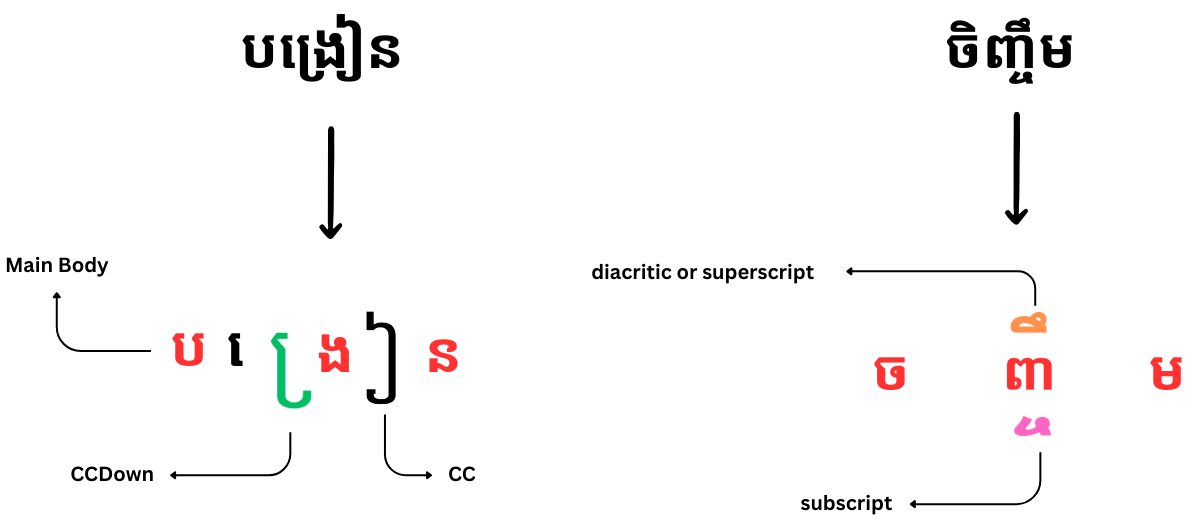
\includegraphics[width=0.87\textwidth]{figures/example_of_text_format.png}
            \begin{minipage}{0.87\textwidth}
                \caption{Example of Khmer text format showing the complexity of character combinations and diacritics \citep{Buoy2022}}.
                \label{fig:text_format}
            \end{minipage}
        \end{figure}
 
    \item \textbf{Inconsistent Word Boundaries:} Khmer lacks standardized word spacing conventions, creating significant segmentation challenges. While English consistently uses spaces between words, Khmer writers apply spacing inconsistently or omit it entirely. This variability makes it extremely difficult for OCR systems to determine word boundaries accurately.
    
        \begin{figure}[H]
            \centering
            
\includegraphics[width=0.87\textwidth]{figures/example_of_long_text.png}
            \begin{minipage}{0.87\textwidth}
                \caption{Example of sequential Khmer text showing how characters combine to form syllables and words}
                \label{fig:sequential_text}
            \end{minipage}
        \end{figure}
 
    \item \textbf{Mixed-Language Complexity:} Cambodia's increased English education and international business integration over recent decades has led to widespread mixed-language documents. Signs, textbooks, and digital content frequently blend Khmer and English within single sentences or paragraphs, creating OCR challenges including script transition confusion, conflicting layout patterns, and font inconsistencies \citep{Wilwohl}.
    
        \begin{figure}[H]
            \centering
            
\includegraphics[width=0.87\textwidth]{figures/mix_language_khmer_and_english.png}
            \begin{minipage}{0.87\textwidth}
                \caption{Example of mixed Khmer-English text showing how both languages appear together in modern Cambodian documents}
                \label{fig:mix_language}
            \end{minipage}
        \end{figure}
        
        Current Khmer OCR systems typically target single-language scenarios and struggle with mixed-language content prevalent in modern Cambodia. The scarcity of properly annotated multilingual datasets compounds this challenge, limiting model training effectiveness and recognition accuracy.
 
    \item \textbf{Font Variation Challenges:} While English utilizes approximately 15-25 common fonts according to industry studies from rigorousthemes.com, lifehack.org, and indeed.com, Khmer encompasses numerous visually distinct font families ranging from bold and thick to thin and decorative styles. Models trained on limited font sets often fail when encountering different typefaces, highlighting the need for comprehensive font coverage in training data.
    
        \begin{figure}[H]
            \centering
            
\includegraphics[width=0.87\textwidth]{figures/varianty_of_font.png}
            \begin{minipage}{0.87\textwidth}
                \caption{Examples of the same Khmer text rendered in different fonts, demonstrating the significant visual variations that OCR systems must handle}
                \label{fig:font_variants}
            \end{minipage}
        \end{figure}
 
    \item \textbf{Character Stacking Patterns:} Khmer employs sophisticated vertical and horizontal character stacking to form syllables and words, creating complex spatial relationships that challenge traditional OCR architectures. These multidimensional arrangements require specialized recognition approaches capable of understanding hierarchical character dependencies.
    
        \begin{figure}[H]
            \centering
            
\includegraphics[width=0.87\textwidth]{figures/text_stacking_mixing_language.png}
            \begin{minipage}{0.87\textwidth}
                \caption{Illustration of Khmer text stacking patterns, showing how characters combine vertically and horizontally to form syllables and words \citep{buoy2023khmerocr}}
                \label{fig:text_stacking}
            \end{minipage}
        \end{figure}

        \item \textbf{Ambiguity in Khmer Character Rendering:} Certain Khmer characters, especially subscript forms like subscript DA and subscript TA, can appear visually identical despite having different Unicode encodings. This leads to high intra-class variance and low inter-class variance, making OCR difficult. As shown in Fig.~\ref{fig:khmer_text_ambiguous}, different char but hard to recognize between characters, increasing recognition errors.
        \begin{figure}[H]
            \centering
            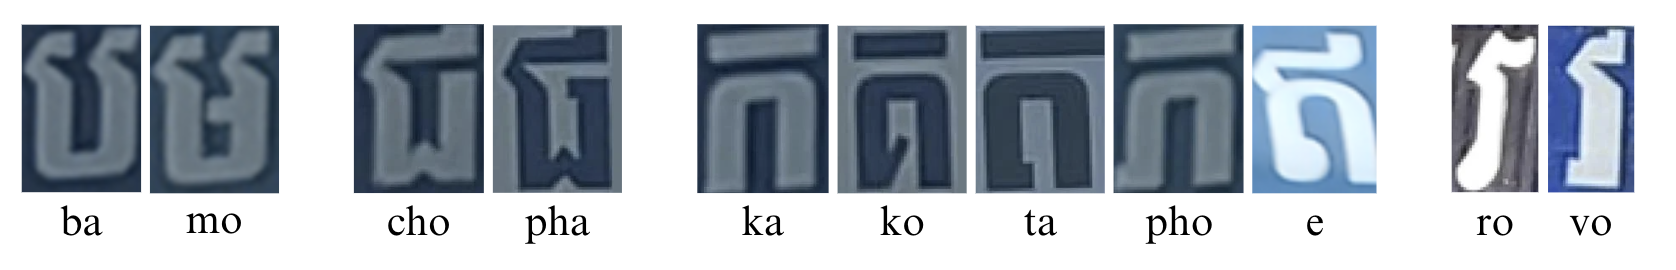
\includegraphics[width=0.87\textwidth]{figures/ambiguous_problem.png}
            \begin{minipage}{0.87\textwidth}
                \caption{Same characters having ambiguous text render \citep{nom2024khmerst}}
                \label{fig:khmer_text_ambiguous}
            \end{minipage}
        \end{figure}
 \end{enumerate}


\section{Aim and Objectives of the Study}
\label{sec:objectives}

Our main goal is to create high performance OCR system 
that can handle mixed writing language of Khmer and 
English in the same document. Our objectives mainly are:

\begin{enumerate}
    \item \textbf{Create a text annotation tool:} Build a tool that can efficiently mark up images with bounding boxes and text labels for both text detection and recognition tasks.

    \item \textbf{Generate synthetic data that actually helps:} To collect real data is expensive and time-consuming, we create millions of synthetic images with different fonts, backgrounds, and realistic distortions that look authentic enough to train the models effectively.

    \item \textbf{Build an end-to-end OCR pipeline:} Customize CRAFT for text detection and TrOCR for recognition, specifically for Khmer script and mixed-language document.

    \item \textbf{Improve over existing solutions:} Aim to achieve better performance and reliable across diverse samples than previous research works or OCR tools such as Tesseract.
    
    \item \textbf{Provide an easy-to-use model:} Deploy our result allowing enthusiast individual easily accessible to experiment with minimal setup. This approach hope to expand the application of OCR in Khmer language.
\end{enumerate}


\section{Rationale of the Study}
\label{sec:rationale}
       This research is motivated by several compelling factors. First, there is an urgent need to digitize and preserve Cambodia's vast textual heritage, including historical documents, educational materials, and cultural artifacts. Without effective OCR technology for Khmer script, this digitization process remains labor-intensive and prone to errors.
       Second, the current limitations of OCR systems for Khmer significantly hinder educational and academic initiatives in Cambodia. Many educational institutions struggle to convert physical textbooks and learning materials into digital formats, impacting accessibility and modernization efforts in education.
       Third, the unique challenges posed by Khmer script from character stacking to the absence of word boundaries present an opportunity to advance the field of OCR technology as a whole. Solutions developed for Khmer may benefit other scripts with similar characteristics.
       Finally, improving Khmer OCR technology aligns with broader digital transformation goals in Cambodia, supporting efforts to preserve cultural heritage while enabling more efficient information processing and accessibility in various sectors.

\section{Limitations and Scope}
\label{sec:limitations}

While this research aims to advance Khmer OCR technology significantly, it is important to acknowledge certain limitations and define the scope of the study:

\begin{enumerate}
    \item The research focuses specifically on printed text of Khmer and English and does not address handwritten in text recognition context, which presents additional challenges requiring further development.
    
    \item The study primarily considers modern Khmer fonts and typography, with limited coverage of historical or decorative text styles.
    
    \item While the system aims to handle various levels of document quality, the extremely degraded or damaged documents may fall outside the scope of reliable recognition.
    
    \item The study focuses on optical character recognition and does not extend to higher-level natural language processing tasks such as semantic analysis or machine translation.
    
    \item Resource constraints may limit the size and diversity of the training dataset, further efforts will be made to ensure sufficient representation of common use cases.
\end{enumerate}

These limitations help maintain a focused research scope while acknowledging areas that may require future investigation.

\section{Structure of the Thesis}
\label{sec:structure}

This thesis is structured into the following chapters:

\begin{enumerate}
   \item \textbf{Introduction}: Establishes the research context, defines objectives, outlines key research questions, explains the study's importance, and sets clear boundaries for the investigation.
   
   \item \textbf{Literature Review}: Examines current OCR technologies, identifies specific challenges in Khmer script processing, and explores relevant deep learning methodologies.
   
   \item \textbf{Dataset Construction}: Describes our data collection process, synthetic data generation techniques, preprocessing methods, and dataset quality evaluation.
   
   \item \textbf{Model Architecture and Experiments}: Details our proposed OCR pipeline, explains model customizations for Khmer script, and outlines training methodologies.
   
   \item \textbf{Results and Analysis}: Reports experimental findings, analyzes performance metrics, and compares our system against existing OCR solutions.
   
   \item \textbf{Discussion and Future Work}: Interprets results, discusses limitations, and identifies opportunities for future research and improvements.
   
   \item \textbf{Conclusion}: Synthesizes key contributions, summarizes main findings, and highlights the broader impact on Khmer OCR development.
\end{enumerate}

Each chapter progressively builds on previous sections to deliver a complete investigation of advanced Khmer OCR technology development.

}
\chapter{Literature Review}
\phantomsection
\label{ch:literature}


\vspace{-1cm}
\setlength{\parindent}{0pt}
\vspace{0.3cm}


\section{Khmer Script Overview}
\phantomsection
\label{sec:Khmer-overview}

{\englishfont\fontsize{13.5pt}{17pt}\selectfont
​ ​ ​ ​ The Constitution of Cambodia establishes Khmer as the 
official language, making accurate digital processing of
Khmer documents crucial for national 
development \citet{Accuracy_Improvement}.
Khmer serves as the primary medium for education, government, 
and cultural expression for over 17 million 
speakers. Unlike Latin-based languages, the Khmer script is an abugida system 
in which each consonant is attached to an inherent 
invisible vowel \citep{buoy2023khmerocr}. One of the main reasons is
the complexity of Khmer characters, which consist of 33 consonants,
16 dependent vowels, and 14 independent vowels and 13 
diacritics \citet{nom2024khmerst}. 


\begin{figure}[H]
  \centering
  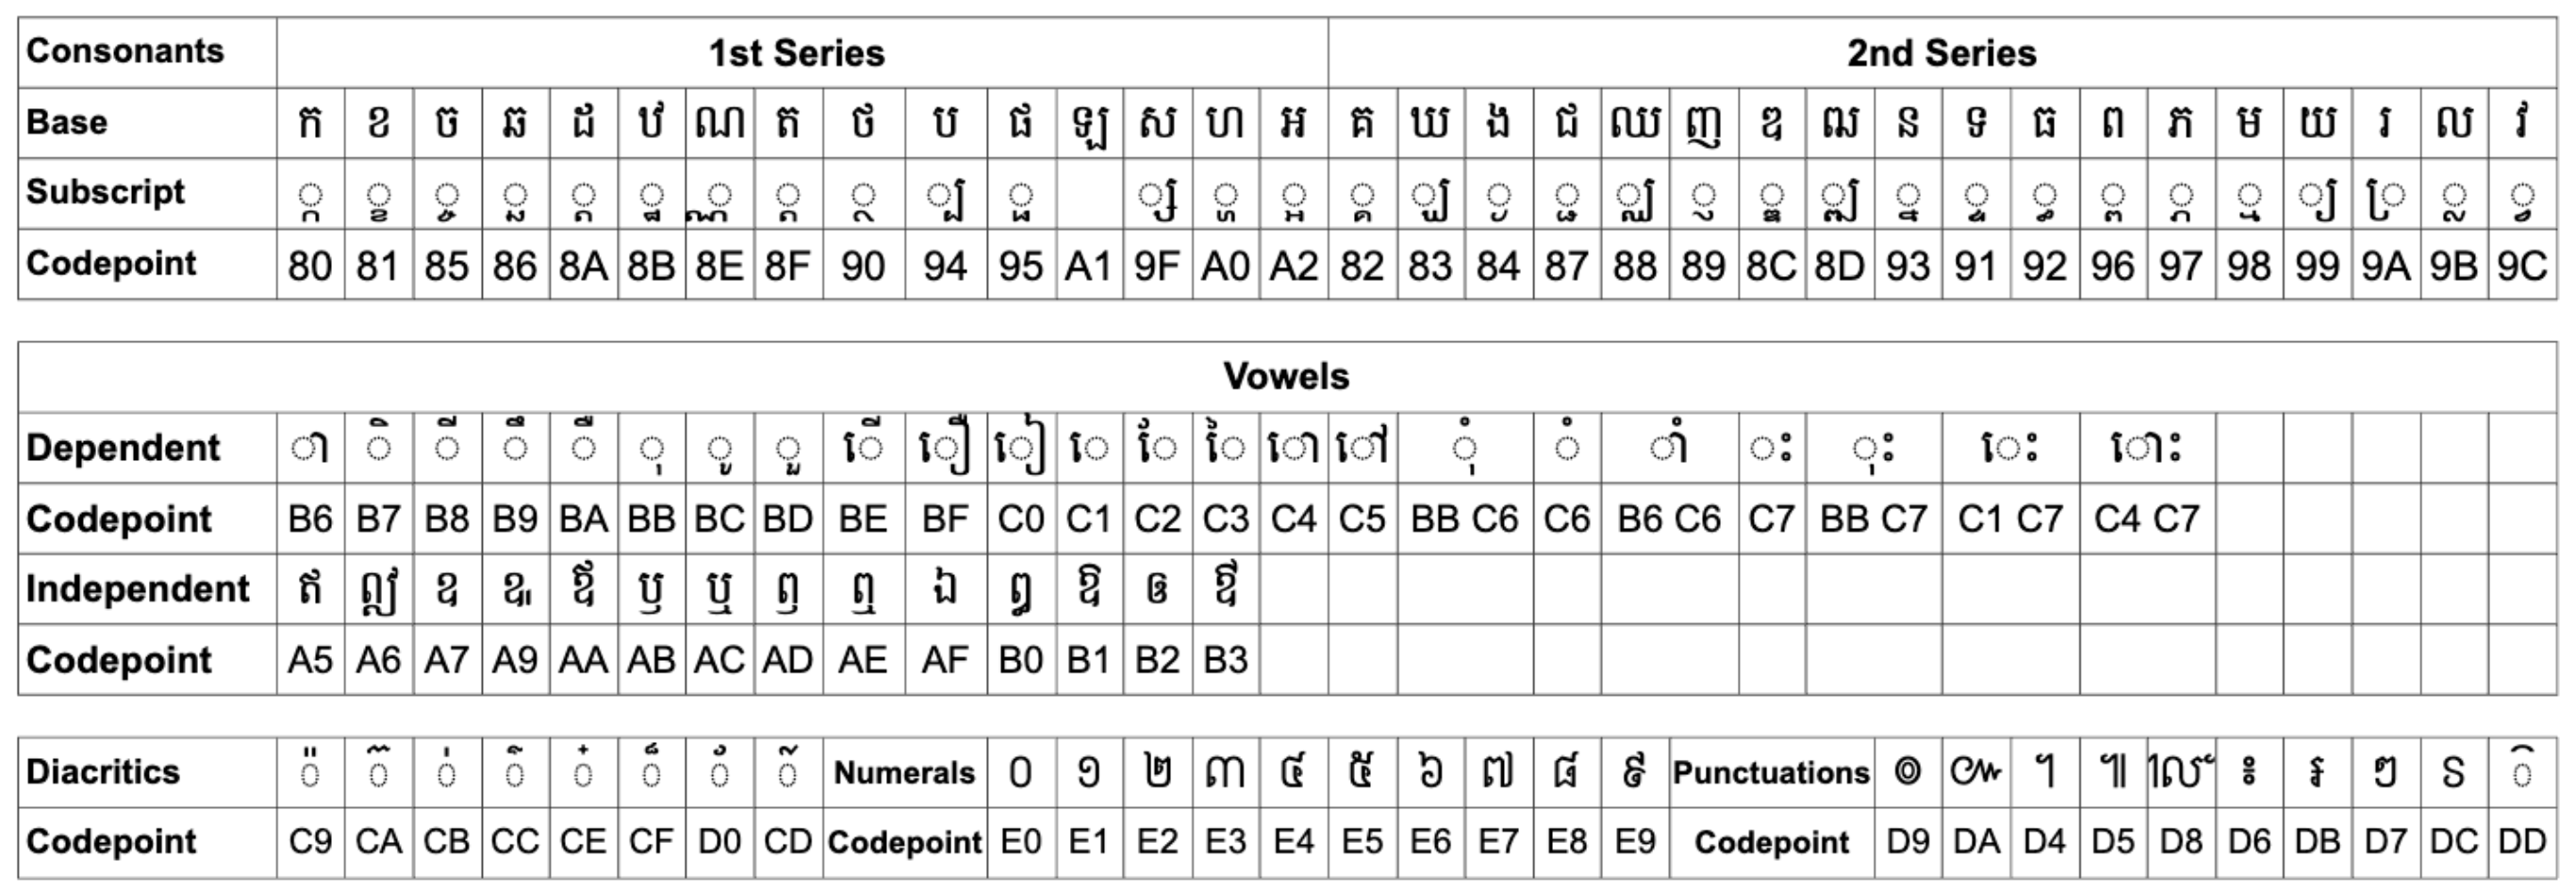
\includegraphics[width=\textwidth]{figures/khmer_alphabet.png}
  \caption{The Unicode point representation of the entire 
  Khmer alphabet, including consonants, vowels, diacritics, 
  and punctuation. Adapted from}
  \label{fig:khmer_alphabets}
\end{figure}

In many Khmer fonts, the subscript forms of certain 
letters (especially DA vs TA, and some other diacritics ) are nearly indistinguishable 
because they both reduce to a small loop shape beneath the base consonant.
Even if they look the same, the actual 
characters used are different in code. This is matter in
search engine, NLP, OCR, and other systems. \citet{Ansary}

\begin{figure}[H]
  \centering
  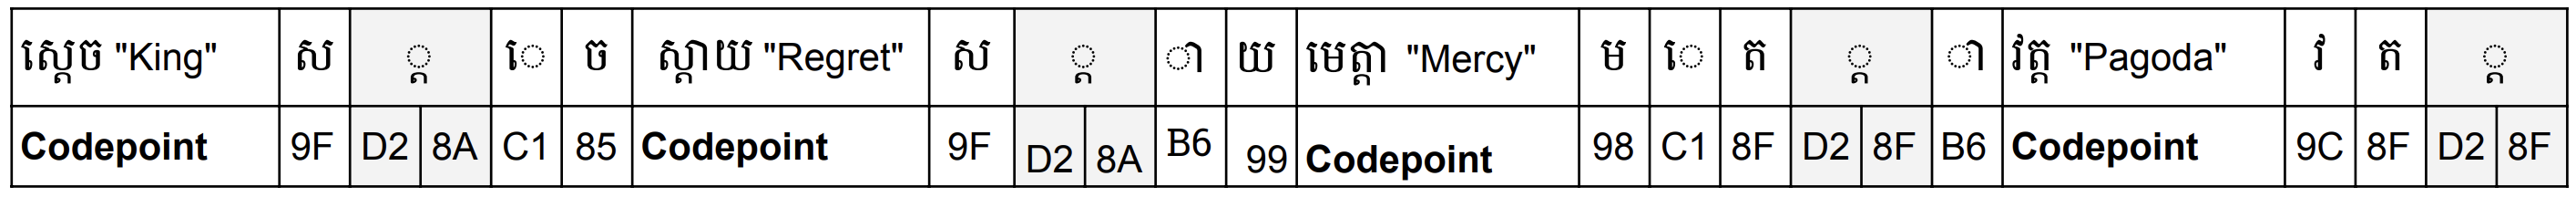
\includegraphics[width=\textwidth]{figures/khmer_word_codepoint.png}
  \caption{The Unicode point representation of word forms using 
  "coeng (U17D2)". For the first two words, they use the 
  subscript DA; for the last two words, they use the 
  subscript TA, but both appear the same, while the Unicode 
  points are different.}
  \label{fig:khmer_codepoints}
\end{figure}


\begin{figure}[H]
  \centering
  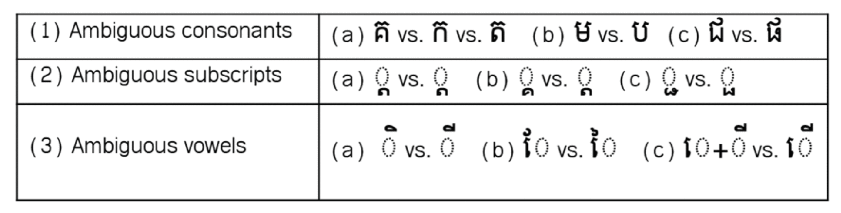
\includegraphics[width=\textwidth]{figures/Ambiguous_characters.png}
  \caption{Ambiguous characters: (1) consonants, (2) subscripts, and (3) vowels. \citet{buoy2023khmerocr}}
  \label{fig:Ambiguous_characters}
\end{figure}

\section{Definition of Optical Character Recognition (OCR)}
\phantomsection
\label{sec:ocr-definition}
​ ​ ​ ​ Optical Character Recognition (OCR) is a field of computer vision and pattern recognition
 that focuses on the automatic identification and digitization of printed or handwritten 
 text from images, scanned documents, or other visual media \citep{singh2012survey}. 
 OCR systems aim to convert visual representations of text into machine-encoded formats, 
 enabling automated indexing, editing, and data extraction \citep{muaz2015khmerocr}.

Modern OCR technology has evolved significantly from its early rule-based and 
template-matching
roots to incorporate advanced machine learning techniques, particularly deep learning,
which allow for improved accuracy in character detection, segmentation, 
and classification across 
diverse languages and scripts.

OCR systems typically consist of several key components: 
image preprocessing (e.g., noise removal, binarization), 
text detection, character segmentation, feature extraction, 
and recognition. These systems must be adapted to handle various 
font styles, image distortions, complex layouts, and script-specific 
features. While OCR for Latin-based languages has become highly accurate, 
extending such systems to Non-Latin scripts such as Khmer remains a 
significant research challenge due to unique linguistic and structural characteristics.
  

\section{Text Detection}
\phantomsection
\label{sec:text_detection_literature}

  ​ ​ ​ ​  \citet{Hiremath_text_detection} The task of detecting text regions in images is a 
crucial first step in many document analysis pipelines.Character Region Awareness by \citet{Baek}
proposed an efficientand accurate scene text detection approach by incorporating character region 
masking and attention. 

\citet{Hiremath_text_detection} Some other popular research Methodology for text detection and 
highly cited text detection algorithms such as:

EAST (Efficient and Accurate Scene Text Detector) \citet{Zhou} uses a fully convolutionalnetwork to 
directly predict word or text line bounding boxes along with their orientation. 
It was one of the first modern deep learning models for this task. TextBoxes++ \citet{TextBoxes}
extended the TextBoxes model with more powerful convolutional features and anangle 
vector to better handle oriented and curved text instances.  CRAFT (CharacterRegion Awareness for 
Text Detection) \citet{Baek} akes a different approach, using a regionscore map to localize 
individual character regions which are then grouped into words/text lines.
Mask TextSpotter \citet{TextSpotter} combines semantic segmentation + attention-based 
recognition to directly read text of any shape from natural scenes all in one unified model.
TextFuseNet \citet{ijcai2020p72} is detects text by extracting and fusing features 
at three levels: character-level, word-level, and global-level. It uses a semantic segmentation 
branch for global context, detects characters and words through a modified Mask R-CNN pipeline, 
and combines all levels using a multi-path fusion architecture. This fusion enriches the text 
representation, enabling the model to better localize and segment text instances of arbitrary shapes.
ABCNet \citet{ABCNet} have been proposed which aim to jointly optimize text detection and 
recognition in a unified architecture. Such unified frameworks potentially allow the two tasks 
to benefit from each other during training. 

% Define a custom column type for better control
\newcolumntype{L}[1]{>{\raggedright\arraybackslash}p{#1}} % left-aligned fixed width
\newcolumntype{C}[1]{>{\centering\arraybackslash}p{#1}}   % centered fixed width

\begin{table}[H]
  \centering
  \caption{Text Detection Accuracy}
  \begin{tabularx}{\linewidth}{|L{3.5cm}|L{2.5cm}|L{2.5cm}|C{2cm}|C{2cm}|C{2cm}|}
    \hline
    \textbf{Model} & \textbf{Backbone} & \textbf{Dataset} & \textbf{Recall (\%)} & \textbf{Precision (\%)} & \textbf{F1-score (\%)} \\
    \hline
    EAST* & VGG-16 & ICDAR 2015 & 78.3 & 83.3 & 80.7 \\
    He et al. & ResNet-50 & ICDAR 2015 & 80.0 & 82.0 & 81.0 \\
    R2CNN & VGG-16 & ICDAR 2015 & 79.7 & 85.6 & 82.5 \\
    TextSnake & VGG-16 & ICDAR 2015 & 80.4 & 84.9 & 82.6 \\
    TextBoxes++* & VGG-16 & ICDAR 2015 & 78.5 & 87.8 & 82.9 \\
    EAA & ResNet-50 & ICDAR 2015 & 83.0 & 84.0 & 83.0 \\
    Mask TextSpotter & ResNet-50 & ICDAR 2017 & 81.2 & 85.8 & 83.4 \\
    PixelLink* & VGG-16 & ICDAR 2017 & 82.0 & 85.5 & 83.7 \\
    RRD* & ResNet-50 & ICDAR 2017 & 80.0 & 88.0 & 83.8 \\
    Lyu et al.* & ResNet-50 & ICDAR 2017 & 79.7 & 89.5 & 84.3 \\
    FOTS & ResNet-50 & ICDAR 2017 & 82.0 & 88.8 & 85.3 \\
    CRAFT & VGG-16 & ICDAR 2015 & 84.3 & 89.8 & 86.9 \\
    \hline
  \end{tabularx}
  \caption*{Source: Results sourced from the CRAFT research paper \cite{Hiremath_text_detection}. 
  Results are reported on quadrilateral-type datasets such as ICDAR. 
  Asterisks (*) denote results based on multi-scale tests. 
  The table compares various scene text detection models including the CRAFT model used in the proposed system across key performance metrics such as precision, recall, and F1-score.}
  \label{tab:text_detection_accuracy}
\end{table}


\section{Khmer Optical Character Recognition (OCR)}
\phantomsection
\label{sec:khmer_OCR_literature}

Most previous work on Khmer OCR are based on complex character segmentation,
standalone character classification, character re-assembling,
word-level or short sentence recognition, single language and some research has focus only
text recognition from the image without any pre-processing steps or text
detection step.

\begin{figure}[H]
  \centering
  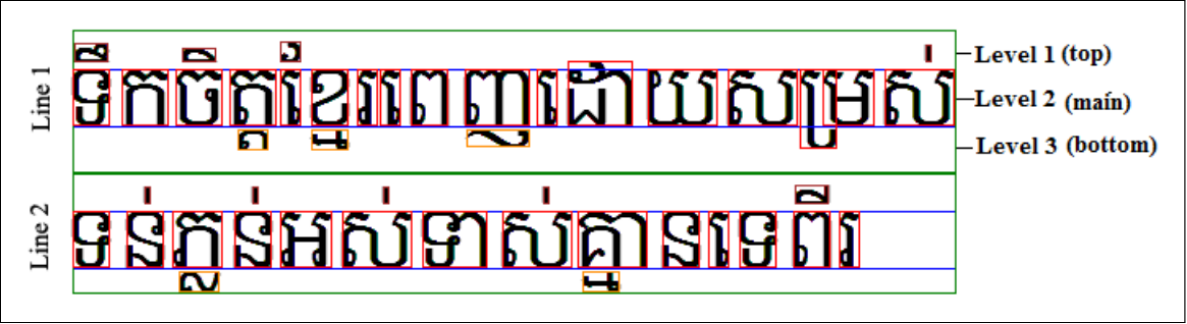
\includegraphics[width=\textwidth]{figures/khmer_char_segmentation.png}
  \caption{Line \& Character Segmentation \citet{Sok&Taing2014}}
  \label{fig:khmer_character_segmentation}
\end{figure}

\begin{figure}[H]
  \centering
  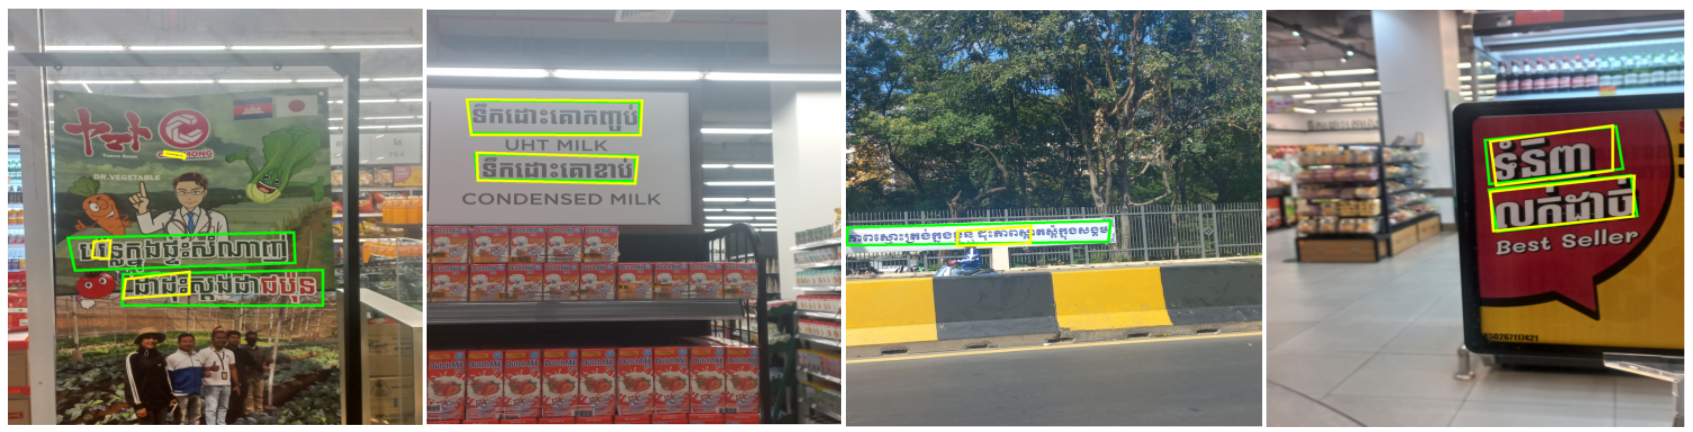
\includegraphics[width=\textwidth]{figures/single_language_only.png}
  \caption{Detection results from YOLOv1 enhanced with CNN: 
  the model predicts the text area in each image by 
  drawing bounding boxes on Khmer language only. \citet{nom2024khmerst}}
  \label{fig:single_language_only}
\end{figure}


​ ​ ​ ​ \citet{CheyFirstOCR} The first significant research on Optical Character Recognition (OCR) 
for Khmer script was proposed in 2006, marking a foundational contribution 
to Khmer language digitization. The study addressed critical challenges 
inherent to Khmer printed characters, notably the variation in character 
shapes across fonts and the high visual similarity between certain 
characters. To overcome these issues, the authors introduced a novel 
recognition method utilizing Wavelet Descriptors. The approach involved 
transforming printed character images into their skeleton forms, 
then converting these skeletons into the temporal domain. Character 
templates were generated using wavelet coefficients from a training set, 
and recognition was performed through a deformable wavelet descriptor 
and a Euclidean distance classifier. The recognition process selected 
the template with the smallest distance to the input character as the 
result. Interestingly, deformation was later excluded from the final 
method due to its adverse impact on distinguishing similar characters. 
Experimental evaluation demonstrated promising results: recognition 
rates of 92.85\%, 91.66\%, and 89.27\% for 22-point, 18-point, and 
12-point font sizes respectively, across 10 Khmer fonts. A second 
test used a 21-page document scanned at varying resolutions 
(150, 300, 600 dpi) and fax inputs, achieving recognition rates 
of 92.99\% at 300 dpi, 88.61\% at 150 dpi, and 80.05\% for faxed documents. 
This pioneering work laid the groundwork for future Khmer OCR systems 
and remains a landmark study in Khmer script recognition.

\citet{Sok&Taing2014} The second significant research on 
Khmer Optical Character Recognition (OCR) introduces a Support 
Vector Machine (SVM)-based approach for printed Khmer character 
recognition in bitmap documents. Given the inherent complexity 
of the Khmer script which includes 74 alphabets and the potential 
for up to five vertical levels in word compounds the study focuses 
on identifying the most effective SVM kernel for classification.
The proposed method evaluates three SVM kernels: Gaussian, Polynomial, 
and Linear. Rather than training on large datasets, the system adopts 
a modular approach, segmenting characters into smaller parts. Each 
segment is transformed into a binary matrix, with 1s representing 
black pixels and 0s for whitespace. Feature extraction is applied 
to these matrices for SVM training and classification.
Following recognition, post-processing rules are employed to merge 
character clusters and correct common misclassifications based on 
character levels. The training utilized one font ("Khmer OS Content") 
at 32pt and tested recognition performance across three font sizes 
(28pt, 32pt, and 36pt). The results demonstrated strong accuracy
98.17\% for 28pt, 98.62\% for 32pt, 98.54\% for 36pt.
The Gaussian kernel outperformed the other kernels, confirming its 
suitability for Khmer character recognition. This study highlights 
the effectiveness of machine learning-based OCR for complex scripts 
like Khmer and marks a major advancement over earlier template-based 
systems.

\citet{Meng_Hann_2014} proposed a Khmer Character Recognition (KCR) 
system utilizing artificial neural networks to address the complexity 
of recognizing individual Khmer script characters. Developed in a 
MATLAB environment, the system integrates a Self-Organizing Map (SOM) 
for unsupervised clustering with a Multilayer Perceptron (MLP) 
trained via the backpropagation algorithm for supervised classification. 
The recognition process follows a two-stage pipeline: first, the input 
image resized to 20×20 pixels is categorized by the SOM into one of 
nine coarse groups. Then, each group is assigned to a dedicated MLP 
model, which performs fine-grained classification into one of 82 
target classes, including Khmer consonants, vowels, and numerals. 
This modular approach aims to enhance classification efficiency by 
narrowing the decision space for each MLP. The system achieved an 
average recognition accuracy of 65\% on the training dataset and 
30\% on the testing dataset, highlighting both the potential and 
the challenges of neural network-based Khmer OCR at the time.

\citet{Muaz2015} This study presents a comprehensive OCR system for 
printed Khmer text using the HTK Toolkit, covering the full 
pipeline of pre-processing, segmentation, recognition, and mapping. 
The system is tailored for the widely used Limon S1 font at 22pt and 
introduces a structural segmentation approach that decomposes 
characters into five categories: Main Body, SuperScript, SubScript, 
CCDown, and Complex Character (CC). Feature extraction relies on 
vertical framing and Discrete Cosine Transform (DCT), with 
classification handled by Hidden Markov Models (HMMs). 
The system was trained on over 35,000 labeled shape samples and 
evaluated on 10 pages of scanned newspaper text, achieving an 
overall recognition rate of 96.34\%. While the results are promising, 
the system is limited by its reliance on a single font style and size, 
making it less robust to font variation. Additionally, recognition 
performance drops for complex shapes like CC (70.88\%) and depends 
heavily on manually crafted mismatch and rule files for post-processing, 
indicating scalability and generalization challenges for real-world 
applications involving diverse document types and fonts.

\citet{Valy_8563219} proposed a character-level Convolutional Neural 
Network (CNN) model for recognizing ancient Khmer script from digitized 
palm leaf manuscripts. The study focuses on two core tasks: 
isolated character recognition and word-level glyph localization. 
For the character recognition task, a CNN architecture comprising 
three convolutional blocks followed by a linear classifier was 
developed. The output layer of the network predicts one of 106 
character classes, achieving a reported test accuracy of 95.96\%. 
In addition to CNNs, the study also explores other neural 
architectures including LSTM-RNN and hybrid CNN-RNN models. 
For the word-text image recognition task, the authors leveraged 
both one-dimensional and two-dimensional RNNs to handle the complex 
spatial structure of Khmer script and to localize glyphs within 
variable-length text patches. This research highlights the potential 
of deep learning approaches in historical Khmer OCR, particularly in 
handling the challenges posed by degraded manuscripts and complex 
writing structures.

\citet{Annanurov_2018} conducted a pilot study on Khmer handwritten 
symbol recognition, focusing on the use of Convolutional Neural 
Networks (CNNs) for digitizing large-scale handwritten document corpora. 
The study used image data from six handwriting datasets containing 
33 Khmer consonants and 17 vowels, forming a total of 561 syllables. 
For consonant recognition, the authors trained 33 individual CNNs one 
for each root radical which were later integrated into a recognition 
assembly. The performance of the CNN-based model was evaluated against 
two alternative systems: an artificial neural network (ANN) using the 
full feature set, and another ANN with reduced feature dimensions. 
Feature extraction techniques such as two-dimensional Fourier 
transformation (FT2D) and Gabor filters were employed for dimensionality 
reduction. The CNN-based approach achieved a recognition accuracy of 
up to 94.85\%, outperforming the ANN-based models. However, the system 
was limited to recognizing only Khmer consonants, without support for 
vowel or syllable-level recognition.

\citet{sokphyrum2019khmer} fine-tuned the Tesseract OCR engine 
(version 4.0) to improve recognition of Khmer Unicode and legacy 
Limon fonts. Tesseract 4.0 employs a deep convolutional recurrent 
neural network with a connectionist temporal classification (CTC) 
loss function and attention mechanism, enabling it to recognize entire 
text-line images. The fine-tuning process involved training on 14 Khmer 
Unicode fonts and 20 pre-Unicode Limon fonts (all at 12pt size). 
The ISRI Analytic Tools were used to evaluate OCR accuracy at both 
the character level (CHL) and cluster level (CLL) by comparing OCR 
outputs to ground truth text. The Khmer pre-trained engine achieved 
an average accuracy of 87.49\% at the character level and 89.43\% at 
the cluster level on Unicode fonts, while legacy Limon fonts yielded 
a significantly lower median accuracy of 62.27\%. After fine-tuning, 
recognition accuracy reached up to 90\% for specific fonts, demonstrating 
the potential of domain-specific adaptation to enhance OCR performance 
for complex scripts like Khmer.


\citet{Buoy2022} Khmer printed character recognition presents significant 
challenges due to the script's complex structure, including stacked consonants, 
dependent vowels, and diacritics placed in various positions. Traditional approaches, 
such as SVMs, wavelet-based templates, and CNNs, have largely focused on recognizing standalone 
characters and depend heavily on accurate segmentation, making them less robust for noisy or 
continuous text-line images. Tesseract OCR, though improved with deep neural networks 
and CTC loss, still performs poorly on heavily augmented images with a reported Character 
Error Rate (CER) of 35.9\%. In contrast, the reviewed study introduces an end-to-end 
attention-based Sequence-to-Sequence (Seq2Seq) model that directly maps entire text-line 
images to character sequences without needing pre- or post-processing. Trained on 3 million 
synthetically generated and augmented images across multiple Khmer fonts, the model 
achieved a CER of 0.7\% on noisy images and 0.24\% on clean images, significantly 
outperforming existing methods and demonstrating the effectiveness of attention mechanisms 
and deep learning for low-resource scripts like Khmer.

\citet{nom2024khmerst} The Khmer script poses significant challenges for scene text detection 
and recognition due to its complex structure involving stacked consonants, multiple diacritics, 
subscript characters, and the lack of explicit word boundaries. To address the scarcity of 
resources for this low-resource language, this study introduces KhmerST, the first annotated 
scene-text dataset for the Khmer language, consisting of 1,544 real-world images captured 
from various public settings in Cambodia. Unlike existing synthetic Khmer datasets, 
KhmerST includes indoor and outdoor images with diverse fonts, orientations, and 
background conditions, and provides polygon-based line-level annotations for more accurate 
localization. Benchmarking with YOLO models shows that YOLOv8 performs best in detection 
tasks due to its ability to handle small and variable text elements, while in recognition 
tasks, both TrOCR and Tesseract perform poorly, with TrOCR achieving CER of 0.90 and 
Tesseract CER of 1.30, highlighting the need for Khmer-specific OCR models. The study 
underscores the gap between current OCR systems and the needs of Khmer script recognition, 
calling for future research on synthetic data generation, Khmer-aware model design, 
and multimodal approaches to improve accuracy in real-world applications.

\citet{Rina2025} This research addresses the challenge of Khmer textline recognition, 
which is particularly difficult due to the absence of spaces between words in the Khmer script. 
Unlike Latin-based languages, this structure requires recognition to be performed at the textline level, 
leading to high latency when using autoregressive (AR) decoders that predict one character at a 
time while considering previous characters. In contrast, non-autoregressive (NAR) decoders can decode 
all characters in parallel but lack awareness of character dependencies, resulting in lower linguistic 
accuracy. To solve this, the authors propose an efficient Khmer textline recognition method using an NAR 
decoder, enhanced by Khmer-specific subword modeling. Instead of predicting single characters, the model 
recognizes character clusters (subwords), capturing the syntactic, morphological, and orthographic 
structure of the language implicitly. This design retains the speed of NAR models while improving accuracy. 
Experimental results show that the proposed method outperforms the character-level NAR baseline 
in accuracy and matches or exceeds the AR baseline while maintaining lower latency. However, 
the abstract does not report detailed accuracy or metrics, and access to full experimental results 
requires a subscription, limiting transparency for non-subscribers. This work contributes an 
important step toward faster and more linguistically aware Khmer OCR by bridging the gap between 
speed and accuracy in scene text recognition.

Khmer OCR research has progressed significantly, yet the script’s structural complexity including 
stacked consonants, subscript forms, diacritics, and the absence of spaces between words continues 
to pose major challenges. Early methods relying on wavelet descriptors, SVMs, and HMMs showed moderate 
success but struggled with font variations, segmentation, and real-world noise. Deep learning has 
since enabled end-to-end approaches like attention-based Sequence-to-Sequence (Seq2Seq) models, 
achieving state-of-the-art accuracy with character error rates (CER) as low as 0.24\% on clean 
images and 0.7\% on noisy inputs. However, general-purpose engines like Tesseract still perform 
poorly, especially in scene text scenarios, as highlighted by results from the newly introduced 
KhmerST dataset. A promising direction involves non-autoregressive (NAR) models enhanced with 
Khmer-specific subword modeling, which offer faster inference and comparable or better accuracy 
than autoregressive (AR) models. Despite these advances, many studies lack open access to detailed 
results, and gaps remain in handwritten recognition, font diversity, and domain adaptation. 
Future research must prioritize Khmer-aware model design, synthetic data generation, and robust 
multimodal solutions to improve performance in real-world OCR applications.
    


\begin{table}[H]
\centering
\caption{Summary of Khmer Optical Character Recognition Research}
\renewcommand{\arraystretch}{1.5}
\begin{tabular}{|p{3.5cm}|p{3.8cm}|p{5cm}|p{3.5cm}|}
\hline
\textbf{Author (Year)} & \textbf{Method} & \textbf{Dataset} & \textbf{Performance} \\
\hline
Chey (2006) & WD + EDC & 10 fonts, 21 pages & 89-93\% accuracy \\
\hline
Sok (2014) & SVM & Single font, 3 sizes & 98\% accuracy \\
\hline
Meng (2014) & SOM + MLP & 82 classes & 65\% train, 30\% test \\
\hline
Muaz (2015) & HMM + HTK & 35K samples, 10 pages & 96\% overall \\
\hline
Valy (2018) & CNN & 106 classes on palms & 96\% accuracy \\
\hline
Annanurov (2018) & CNN Assembly & 6 datasets, 561 syllables & 95\% accuracy \\
\hline
Sokphyrum (2019) & Tesseract 4.0 & 34 fonts & 87-89\% (Unicode) \\
\hline
Buoy (2021) & Seq2Seq + Attention & 3M synthetic images & CER: 0.24-0.7\% \\
\hline
Nom (2024) & YOLO + TrOCR & 1.5K real images & CER: 0.90-1.30 \\
\hline
Buoy (2025) & NAR + Subword & Textlines & Better than AR \\
\hline
\end{tabular}
\label{tab:khmer_ocr_summary}
\end{table}


\section{Challenges in Khmer OCR}
\phantomsection
\label{sec:datasets}

Khmer OCR poses numerous technical challenges stemming from the script's unique structure and 
linguistic features. Unlike Latin-based scripts, Khmer characters can include complex stacking 
of consonants (e.g., subscript consonants using Coeng), placement of diacritics, and variable vowel 
positions that appear above, below, before, after, or even wrap around base characters \citep{buoy2021seq2seq}. 
This spatial complexity makes segmentation particularly difficult and often unreliable, 
especially in cluttered or noisy environments. Accurate character separation is further complicated 
by the fact that multiple elements can visually overlap, causing traditional segmentation-based 
approaches to fail.

Font diversity also adds a layer of complexity. Khmer is written using a wide array of fonts, each 
introducing variations in stroke thickness, character proportions, and spacing. These stylistic 
differences can drastically alter a character's appearance, requiring OCR systems to be highly 
font-invariant \citep{buoy2021seq2seq}. Yet, many models are trained on limited font sets, leading 
to poor generalization across unseen styles.

Another critical issue is the scarcity of annotated datasets. As a low-resource language, Khmer lacks 
the extensive labeled corpora available for Latin or Chinese scripts. This data scarcity hampers the 
training of robust models and forces researchers to rely on synthetic data or heavily augmented datasets 
to simulate real-world variability.

Additionally, many legacy OCR systems for Khmer rely on rule-based or modular pipelines with explicit 
character segmentation, manual pre- and post-processing, and assumptions about text structure. These 
approaches are brittle and poorly suited for real-world applications where scanned documents may contain 
noise, skew, blur, uneven lighting, or distorted text lines. Their reliance on handcrafted rules also 
limits scalability and adaptability to other domains.

Lastly, the lack of word boundaries in Khmer where text is often written without spaces presents an 
additional recognition barrier. This linguistic feature necessitates full line-level recognition, 
which increases computational complexity and requires models to understand broader contextual dependencies 
across characters.



\section{Role of Synthetic Data}
\phantomsection
\label{sec:dl-models}

To overcome the challenges associated with data scarcity in Khmer OCR, 
recent studies have emphasized the critical role of synthetic data generation. A prominent 
strategy involves leveraging the open-source \texttt{text2image} utility from the Tesseract OCR 
engine to create high-quality, rendered images of Khmer text lines \citep{buoy2021seq2seq}. 
These images are generated from a curated text corpus that includes a diverse mix of numbers, 
words, phrases, and full sentences, providing broad linguistic coverage.

Multiple commonly used Khmer fonts are applied during rendering to simulate font diversity and 
improve the model's ability to generalize across different typographic styles. Each rendered 
image is converted to grayscale and resized to a fixed height (e.g., 32 pixels) to meet the input 
dimensional requirements of neural network models, while maintaining proportional width to preserve 
text structure.

To emulate real-world conditions and enhance robustness, extensive data augmentation techniques 
are applied. These include Gaussian blurring, morphological operations like dilation and erosion, 
speckle and blob noise injection, background texture overlays, rotational distortions, and random 
concatenation of multiple text-line images. Each augmentation has a 50\% probability of being applied, 
with combinations occurring dynamically during training to maximize variability and minimize overfitting.

The resulting synthetic dataset scales to millions of samples, covering a wide spectrum of distortions, 
font styles, and text structures. This scale and diversity enable deep learning models particularly 
end-to-end architectures such as attention-based Sequence-to-Sequence networks to learn robust 
visual and contextual features, improving performance on both clean and noisy inputs. Ultimately, 
synthetic data serves as a vital resource for building Khmer OCR systems capable of handling the 
script’s inherent complexity in the absence of large, annotated real-world datasets.


\section{Summary of Research Gaps}
\phantomsection
\label{sec:research-gaps}

Despite recent progress in Khmer Optical Character Recognition (OCR), 
several critical gaps persist in the current body of research, hindering the 
development of robust and generalizable systems. First and foremost is the issue of 
data scarcity there is a lack of large-scale, high-quality annotated datasets for Khmer, 
particularly for scene text and handwriting, which restricts model training, benchmarking, 
and cross-domain evaluation. Although synthetic datasets have partially mitigated this, they 
cannot fully replicate the variability and unpredictability of real-world documents. Second, the 
complex structural features of Khmer script such as stacked consonants, overlapping vowel markers, and 
the absence of explicit word boundaries are insufficiently addressed in many existing models, 
especially those adapted from Latin-script OCR frameworks. These models often fail to 
capture the script's spatial dependencies and morphological nuances. Third, font 
variability remains a major bottleneck: Khmer documents are written in a wide range of stylistic 
fonts, and OCR systems trained on limited font sets often generalize poorly. Lastly, there is 
a lack of robustness to real-world document conditions, including noisy backgrounds, image blur, 
skew, and low resolution. Many current systems, including Tesseract and some CNN-based models, 
show significant performance drops under such conditions. Addressing these gaps through 
Khmer-specific model design, comprehensive dataset creation, and more resilient training strategies is 
essential for building high-performance OCR systems tailored to the Khmer language and its 
real-world use cases.

}

\chapter{Dataset Construction}
\phantomsection
\label{ch:dataset}


\vspace{-1cm}
\setlength{\parindent}{0pt}
\vspace{0.3cm}

\section{Khmer Text Data Collection}
\label{sec:text-source}

{\englishfont\fontsize{13.5pt}{17pt}\selectfont

The data collection process began with gathering Khmer word-by-word data from the 
Chuon-Nath Dictionary, which provided over 50,000 words. However, it needs
sentence-level as well, data was also necessary for comprehensive text-line based recognition model. 
To address this, a web scraping script was developed using the BeautifulSoup library 
to collect sentence data from the website khsearch.com. This resulted in the collection 
of approximately 500,000 Khmer sentences.

Upon analyzing the collected data, it was found that there was an imbalance between 
Khmer and English language data. To address this, the Alpha-Word dataset was acquired,
which contained over 300,000 English words. Furthermore, the Google-Word dataset 
was also collected, which provided a large volume of natural language data commonly 
used on the internet. Additionally, the Hugging Face dataset was used to supplement 
the collection with more natural language data.

In total, the dataset collection process yielded over 3.7 million 
character/symbols/words/sentences, including Khmer/English char-level, word-level, 
and sentence-level, this dataset will double by apply different font and diversity. The natural text data from the internet is a crucial role in
OCR model training.

\section{Data Manual Collection}
\label{sec:manualcollection}
In this step we collect dataset manually from the web and other sources. we 
use our own data annotation application to collect the data. The data is not just for Optical 
Character Recognition (OCR) but also for text detection as well, with this tool can be
used to collect dataset flexibility and efficiency that is integrated with commercial OCR API
to collect data faster. The exiting tool for collecting dataset is not flexibility enough in
our case, because we need to collect dataset for both text detection and OCR tasks.

In this step, data was collected around 369 images equal to 7552 bounding boxes, it's can be
used for training with text detection and I used it as testing set for text recognition task.

\begin{figure}[H]
    \centering
    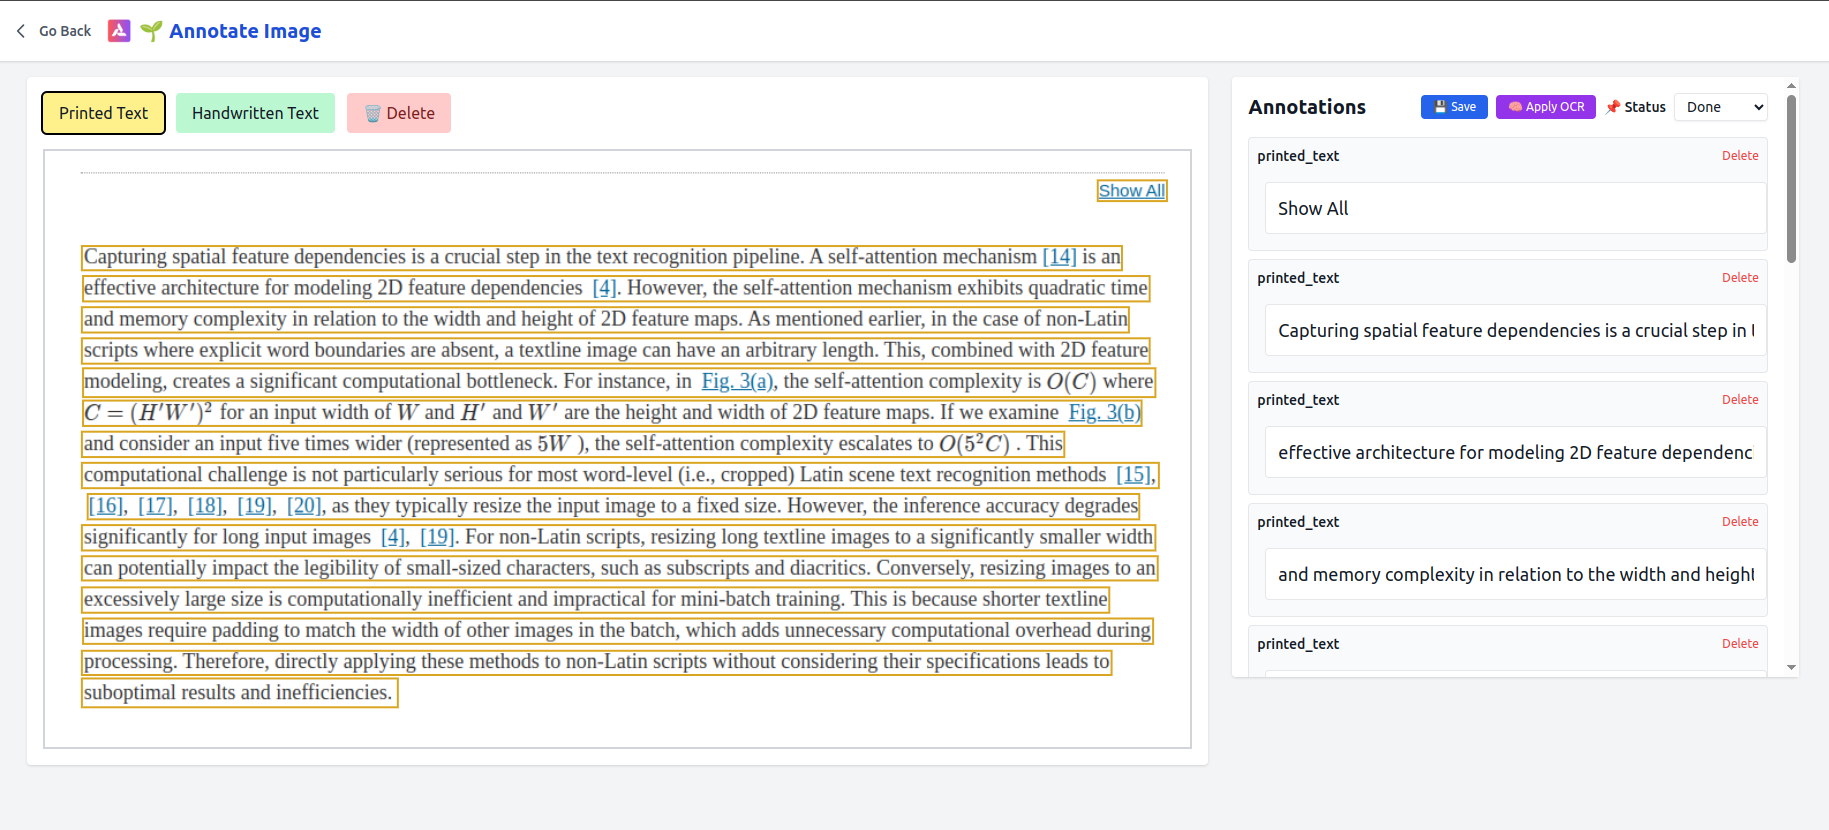
\includegraphics[width=\textwidth]{figures/data_annotation_application.png}
    \caption{Example of a tool to collect dataset combine with text commercial API.}
    \label{fig:data_annotation_tool}
\end{figure}


\section{Text Cleaning and Preprocessing}
\label{sec:preprocessing}
The text data collected from the Chuon-Nath Dictionary, Alpha-Word, 
and Google-Word datasets was found to be clean and required no preprocessing. 
However, the text collected from internet scraping from khsearch.com was not 
clean and required preprocessing to enhance OCR performance. The text data was 
analyzed and any uncommon links or URLs, excessive spacing, tabs, and invisible 
characters were removed. Furthermore, the sentences in the text data were found 
to be too long, so the text data was segmented into word-by-word format using the 
khmer-nltk library and then random sentences were generated from 1 to 125
characters in length, while maintaining the order of the sentences. 
This was done to ensure that the OCR model could predict missing characters 
based on the natural order of the sentences. Additionally, the text data was 
normalized to ensure that all characters were in the same format, which is 
important for OCR performance.
After preprocessing, the dataset was split into two parts: a training set 
and a validation set. The training set was used to train the OCR model, 
while the validation set was used to evaluate the performance of the OCR model.

\begin{figure}[H]
    \centering
    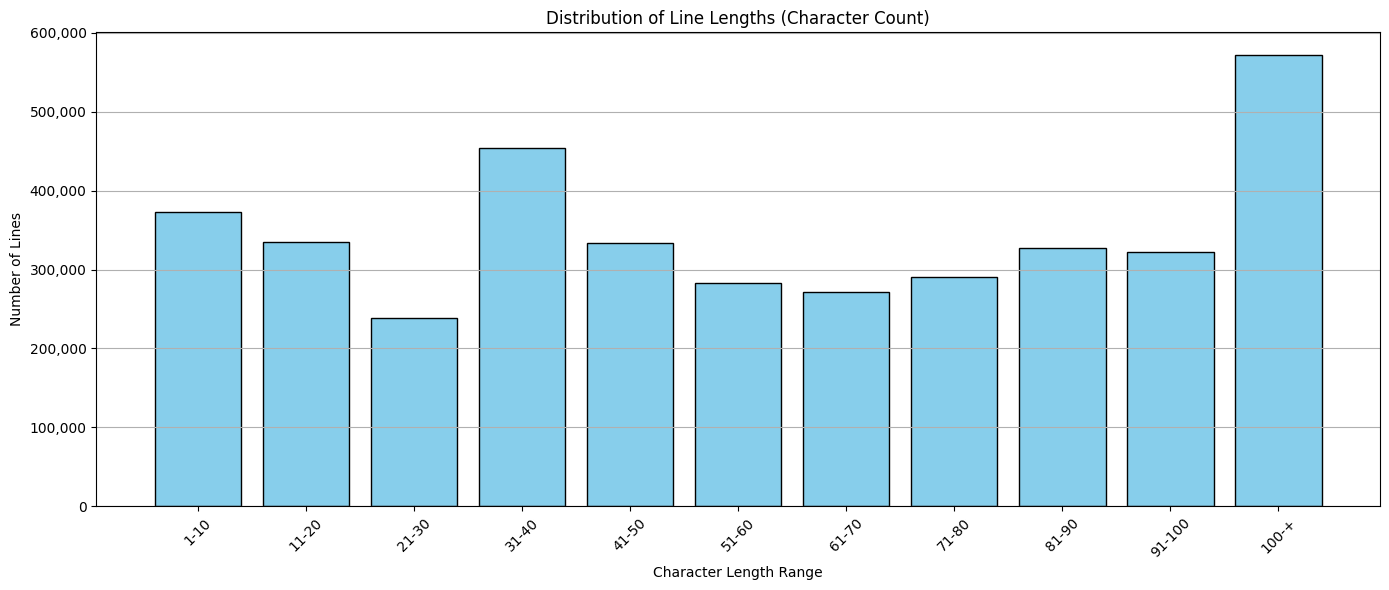
\includegraphics[width=\textwidth]{figures/frequency_of_text_length.png}
    \caption{Frequency of text length in the synthetic dataset, 
    showing the distribution of text lengths. The majority of the text  
    lengths are between 0 to 125 characters.}
    \label{fig:frequency_of_text_length}
\end{figure}



\section{Image Generation Pipeline}
\label{sec:generation}
The synthetic dataset was generated by loading text from data\_khmer\_text.txt line 
by line and applying different fonts using the Pillow library. The aim of this 
step was to generate a wide variety of text styles and fonts, so that the OCR 
model could be trained on diverse text styles. To achieve this, approximately 
20 different font styles were applied to each line of text. Additionally, 
each line was combined with 20 different background images to simulate real-world 
image text. This was done to ensure that the OCR model could recognize text 
regardless of the background of the image.

\begin{figure}[H]
    \centering
    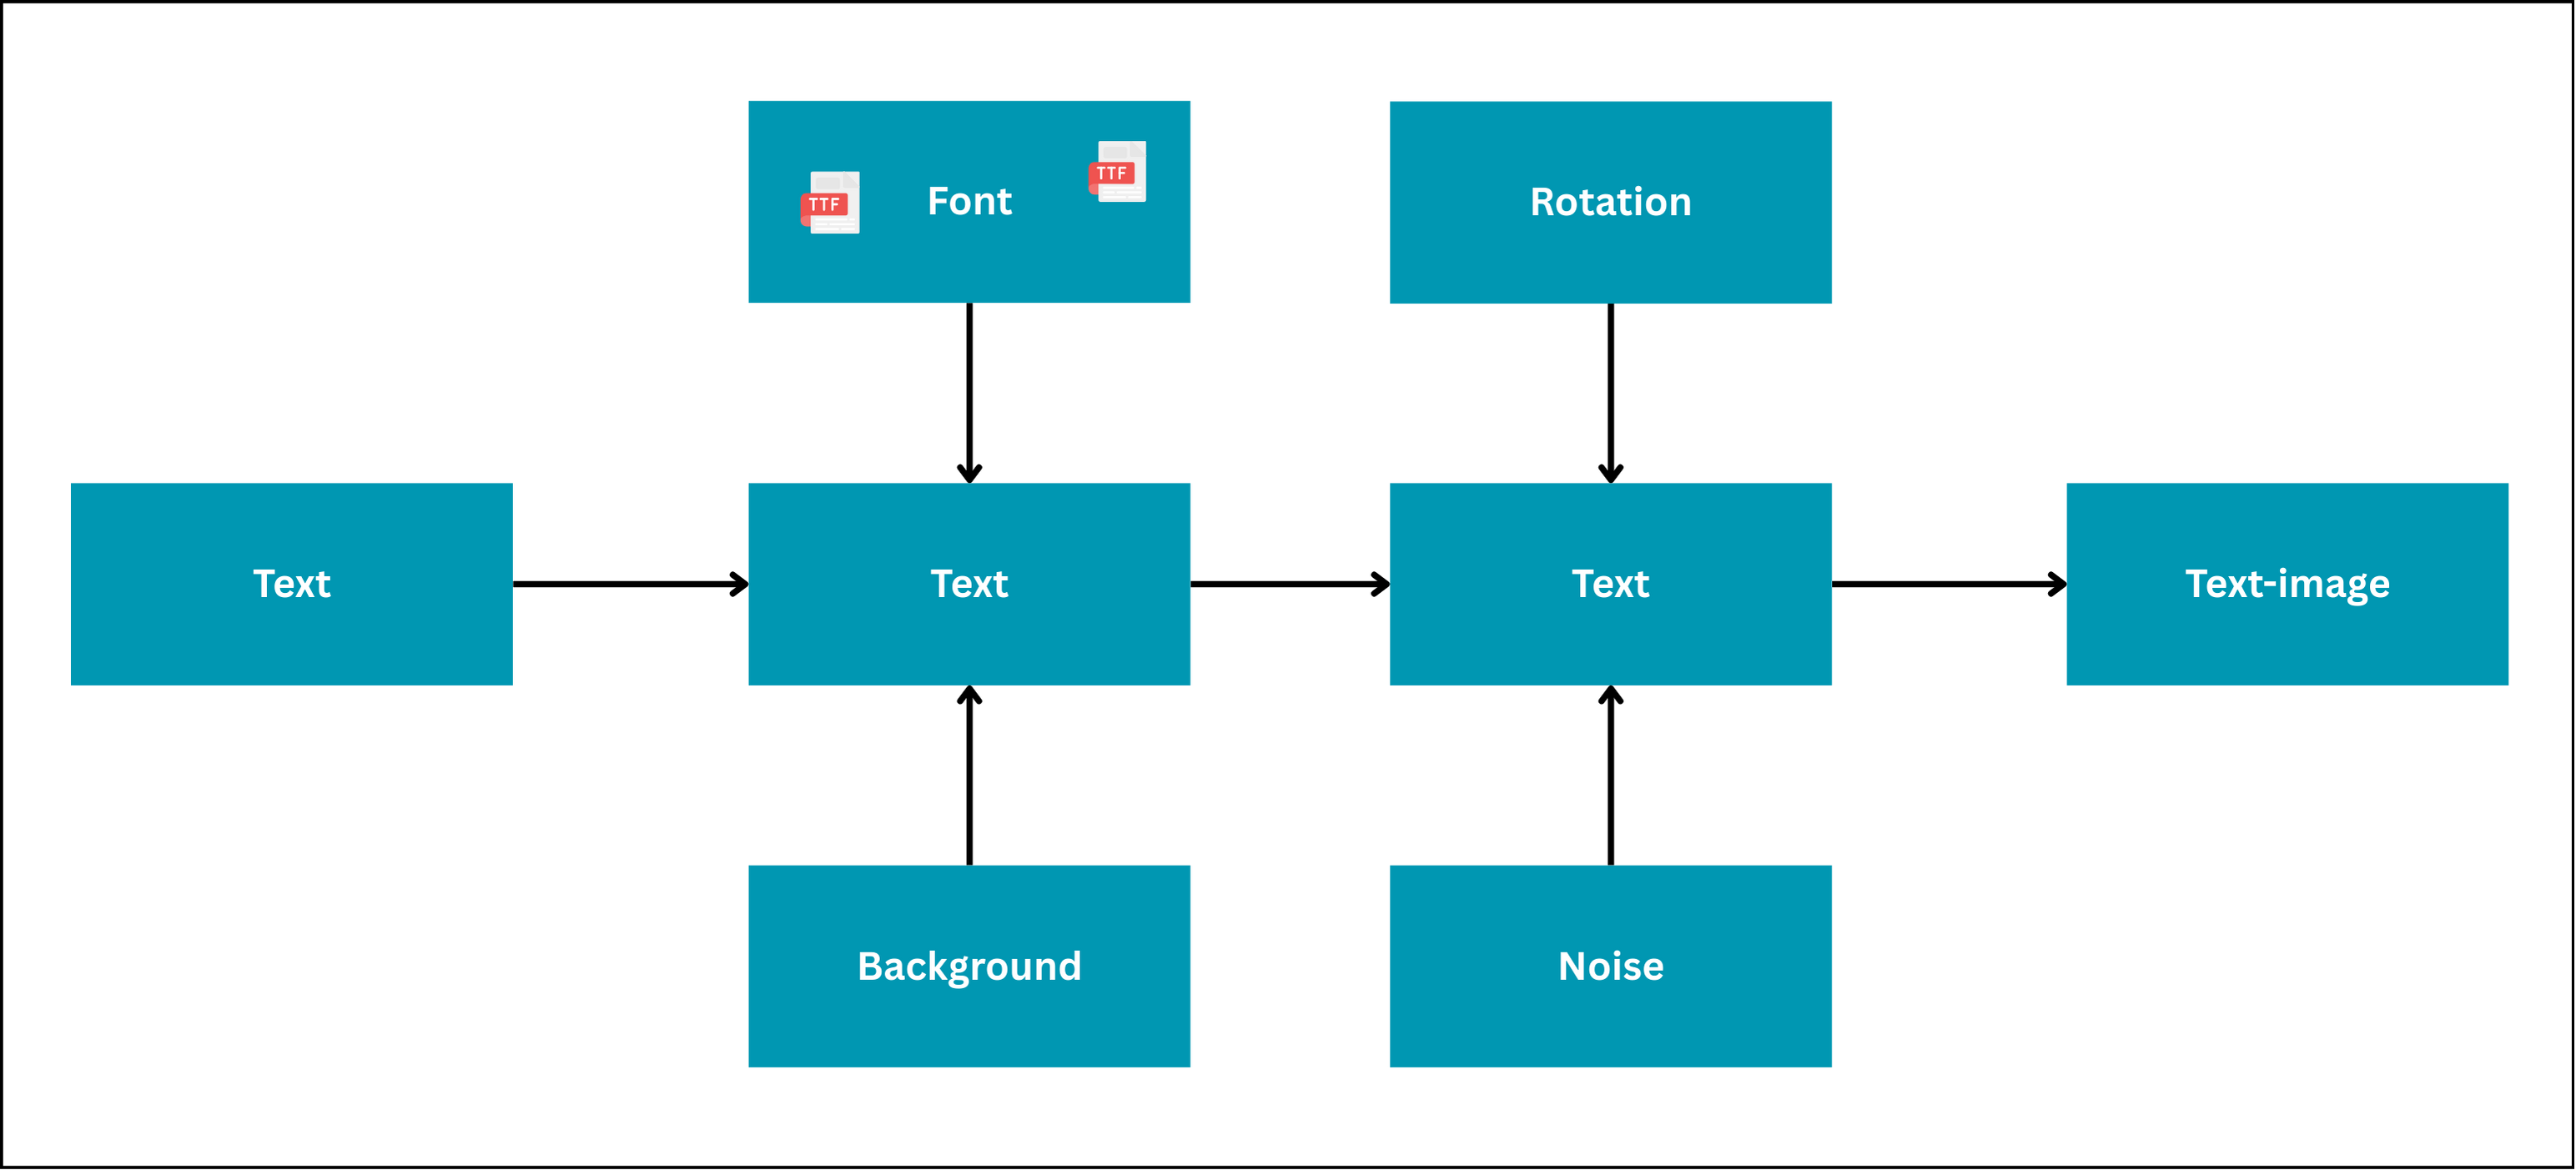
\includegraphics[width=\textwidth]{figures/synthetic_image.png}
    \caption{Example of a synthetic image generated for the OCR training dataset, 
    illustrating the application of random fonts, backgrounds, and noise to simulate 
    real-world conditions.}
    \label{fig:synthetic-image}
\end{figure}


Various types of noise were applied to the text images to simulate real-world 
conditions. This included gaussian blurring, dilation and erosion, blob noise, 
speckle noise, multi-scale noisy backgrounds, random concatenation of augmented 
images, and salt-paper noise. The text on the images was rotated from -3 to 3 
degrees to simulate variations in text orientation. Additionally, margins of 
1-5 pixels were randomly added to the text images to account for inconsistent 
text detection. As each text line could generate two images, the total number 
of images produced was 7.4 million.


\begin{figure}[H]
    \centering
    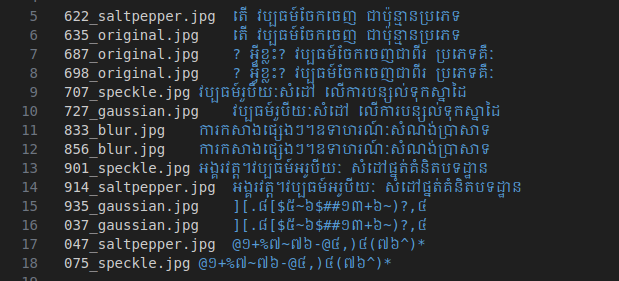
\includegraphics[width=\textwidth]{figures/result_after_generation.png}
    \caption{The annotated result of a synthetic image generated for the OCR training dataset.}
    \label{fig:synthetic-image_output}
\end{figure}


The resulting synthetic dataset contained 7.4 million images, each with a unique 
combination of font, background, and noise. The images were designed to simulate 
real-world conditions, such as text orientation, text margins, and various types of 
noise. The application of these techniques resulted in a high-quality synthetic dataset 
that was suitable for training the OCR model. When examining the resulting synthetic 
dataset, it is clear that the images are highly diverse and realistic, with a wide range 
of font styles, colors, and backgrounds. Additionally, the noise types and levels are 
varied, which will help to improve the robustness of the OCR model when trained on 
this dataset. It is also clear that the images are of high quality, with crisp and clear 
text and minimal artifacts. The overall quality of the dataset is high, which will help 
to ensure that the OCR model is well-trained and can accurately recognize text in a 
variety of contexts.

\begin{figure}[ht]
    \centering
    
\includegraphics[width=\textwidth]{figures/resutl_synthetic_dataset.png}
    \caption{Result of the synthetic dataset generation pipeline, showing the diversity of fonts, backgrounds, and noise types.}
    \label{fig:result_synthetic_dataset}
\end{figure}


}
\chapter{Model Architecture and Experiments}
\phantomsection
\label{ch:experiments}


\vspace{-1cm}
\setlength{\parindent}{0pt}
\vspace{0.3cm}

\section{End-to-End Khmer OCR Network system}
\label{sec:end_to_end_khmer_ocr_sysetm}

{\englishfont\fontsize{13.5pt}{17pt}\selectfont

We propose an end-to-end Khmer OCR pipeline that combines the CRAFT model 
for text detection with the TrOCR model architecture developed by Microsoft 
for text recognition. We have customized and adapted the system to support 
both Khmer and English languages. The pipeline takes an input image, applies 
the CRAFT model to detect and crop individual text-line regions, and then 
feeds each text-line image into the TrOCR model.
The TrOCR model operates in an auto-regressive manner, decoding one character 
at a time until it reaches the end-of-sequence token. This approach allows the 
system to handle variable-length input text-lines without any predefined limit, 
as long as the input fits within the model’s maximum token capacity.
This is a high-level description of the system architecture. Importantly, 
our pipeline operates without any preprocessing steps like binarization, 
noise removal, or skew adjustment. It processes raw input images directly, 
handling both detection and recognition seamlessly within a unified end-to-end 
framework.

\section{Experimental Environment and Tools}
\label{sec:environment}

All experiments were conducted on a Linux CLI system with the following hardware
and software specifications listed below:

\begin{table}[H]
    \centering
    \caption{Experimental Setup and Environment Configuration}
    \renewcommand{\arraystretch}{1.4}
    \resizebox{\textwidth}{!}{%
    \begin{tabular}{|p{4.5cm}|p{5.7cm}|p{6.5cm}|}
    \hline
    \textbf{Component} & \textbf{Specification} & \textbf{Purpose} \\[0.2cm]
    \hline
    \multicolumn{3}{|c|}{\textbf{Hardware Configuration}} \\[0.2cm]
    \hline
    Operating System & Ubuntu 20.04 LTS & Stable training large model \\[0.2cm]
    \hline
    GPU Units & 3x NVIDIA RTX 4090 & Parallel computing \\[0.2cm]
    \hline
    VRAM & 24 GB per GPU (72 GB total) & Large model training and inference \\[0.2cm]
    \hline
    System Memory & 256 GB RAM & Great for loading \& processing \\[0.2cm]
    \hline
    \multicolumn{3}{|c|}{\textbf{Software Framework}} \\[0.2cm]
    \hline
    DL Framework & PyTorch & implementation \& training \\[0.2cm]
    \hline
    Model Library & Hugging Face Transformers & Pre-trained architecture access \\[0.2cm]
    \hline
    GPU Acceleration & CUDA & Great for training across GPUs \\[0.2cm]
    \hline
    \multicolumn{3}{|c|}{\textbf{Experiment Management}} \\[0.2cm]
    \hline
    Tracking System & MLflow & Real-time metric logging \\[0.2cm]
    \hline
    Monitored Metrics & CER, Train/Valid Loss & evaluation \& comparison \\[0.2cm]
    \hline
    \end{tabular}%
    }
    \label{tab:experimental_setup}
\end{table}

\section{CRAFT for Text Detection}
\label{sec:craft-complete}

This section presents a comprehensive overview of the CRAFT 
(Character Region Awareness for Text Detection) model implementation, 
covering its architecture, configuration, training methodology, dataset 
preparation, and evaluation metrics.

\subsection{CRAFT Model Architecture}
\label{subsec:craft-architecture}

For the text detection stage, we adopted the Character Region Awareness for Text 
Detection (CRAFT) model, which is a fully convolutional network architecture 
based on VGG-16 with batch normalization is adopted as this architecture's backbone.
The model has skip connections in the decoding part, which is similar to U-net in
that aggregates low-level features. The final output is producing two channels as 
score maps:
\begin{itemize}
\item A \textbf{region score map}, indicating the likelihood of each pixel belonging 
to a character region.
\item An \textbf{affinity score map}, capturing the spatial relationships between 
adjacent characters to form text lines.
\end{itemize}

Unlike traditional text detectors that rely on bounding-box regression, 
CRAFT performs pixel-level predictions to detect the centers of individual 
characters and the affinities between them, allowing it to handle curved, 
rotated, or irregular text effectively. However, in our work, we focus on 
text-line-level detection rather than character-level because Khmer is a 
complex writing system. Many characters are visually dependent, invisible, 
or cannot appear independently, making character-level detection unreliable 
for curved or rotated Khmer text. Since curved text detection relies on accurate 
per-character localization and grouping, CRAFT's character-centric design does 
not perform well on curved Khmer scripts.



\begin{figure}[H]
    \centering
    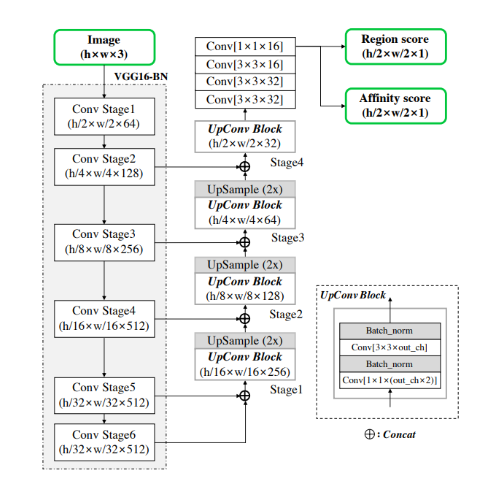
\includegraphics[width=\textwidth]{figures/craft_layer_network.png}
    \caption{Schematic illustration of our CRAFT network architecture.
    \citep{baek2019craft}}
    \label{fig:craft-model}
\end{figure}


\subsection{CRAFT Network Architecture}
\label{subsec:craft-architecture-network}

The Character Region Awareness for Text Detection (CRAFT) model adopts a fully convolutional architecture based on the VGG-16 backbone with batch normalization. It is designed to predict two output maps: the region score map and the affinity score map, representing the center probability of each character and the space between adjacent characters, respectively.

\subsubsection*{Backbone Network: VGG-16}

The first part of the model utilizes VGG-16 \cite{Simonyan} 
as the feature extractor. Let the input image be denoted by 
$I \in \mathbb{R}^{H \times W \times 3}$. The VGG-16 backbone extracts 
hierarchical feature maps:

\[
\begin{aligned}
F_1 &= \text{Conv}_{1\text{-}2}(I) \quad &\text{(features after conv1)} \\
F_2 &= \text{Conv}_{2\text{-}2}(F_1) \quad &\text{(features after conv2)} \\
F_3 &= \text{Conv}_{3\text{-}3}(F_2) \quad &\text{(features after conv3)} \\
F_4 &= \text{Conv}_{4\text{-}3}(F_3) \quad &\text{(features after conv4)} \\
F_5 &= \text{Conv}_{5\text{-}3}(F_4) \quad &\text{(features after conv5)} \\
\end{aligned}
\]

\subsubsection*{Decoder: U-Net-style Feature Fusion}

The decoder employs a U-Net-like architecture \cite{Ronneberger} with skip 
connections to aggregate semantic and spatial information. Starting from $F_5$, 
the features are upsampled and concatenated with features from earlier layers:

\[
\begin{aligned}
F_{54} &= \text{Concat}(\text{Upsample}(F_5), F_4) \\
F_{543} &= \text{Concat}(\text{Upsample}(F_{54}), F_3) \\
F_{5432} &= \text{Concat}(\text{Upsample}(F_{543}), F_2) \\
F_{54321} &= \text{Concat}(\text{Upsample}(F_{5432}), F_1) \\
\end{aligned}
\]

Each fusion step is followed by one or more $3 \times 3$ convolutional layers with ReLU activations. The final decoding stage uses a series of convolution layers:

\[
\text{Conv}_{3\times3\times32} \rightarrow \text{Conv}_{3\times3\times32} \rightarrow \text{Conv}_{3\times3\times16} \rightarrow \text{Conv}_{1\times1\times16}
\]

\subsubsection*{Output Heads}

The final fused features are projected into two separate output maps using $1 \times 1$ convolutions:

\[
\begin{aligned}
S_r &= \sigma(\text{Conv}_{1\times1}^{1}(F_{out})) \quad &\text{(region score map)} \\
S_a &= \sigma(\text{Conv}_{1\times1}^{1}(F_{out})) \quad &\text{(affinity score map)} \\
\end{aligned}
\]

Here, $\sigma$ denotes the sigmoid activation function. 
The region score $S_r$ represents the likelihood that a pixel is at the center 
of a character, while the affinity score $S_a$ represents the connection strength 
between adjacent characters \citet{baek2019craft}.

\subsubsection*{Output Resolution}

The output maps $S_r$ and $S_a$ are of size $H' \times W'$, 
typically at $\frac{1}{2}$ resolution of the input image due to strided 
convolutions and pooling operations in the VGG-16 backbone.










\begin{figure}[H]
    \centering
    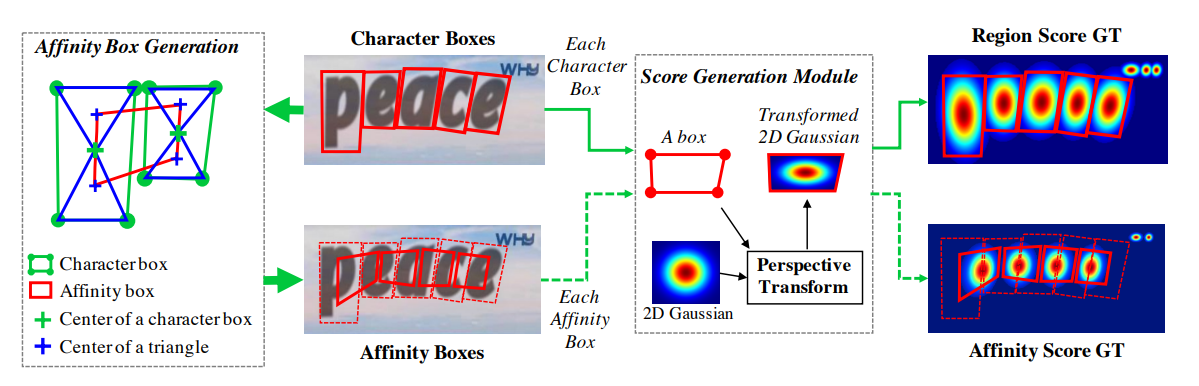
\includegraphics[width=\textwidth]{figures/craft_model_architecture.png}
    \caption{Illustration of ground truth generation procedure in our framework. 
    We generate ground truth labels from a synthetic image that has character level annotations.
    \citep{baek2019craft}}
    \label{fig:craft-model-architecture-detailed}
\end{figure}

The model has 20,770,466 trainable parameters. We used the official 
implementation of CRAFT with some modifications to better support Khmer text,
including the use of a custom dataset and a modified training procedure such as
skip the character labels during training.


\subsection{CRAFT Training Configuration}
\label{subsec:craft-training-config}

The CRAFT model was fine-tuned on a custom Khmer text dataset using fully supervised learning, 
leveraging the strengths of annotated real-world images. The key configuration parameters 
for training the CRAFT model are summarized in Table~\ref{tab:craft-training-config}.

\begin{table}[H]
    \renewcommand{\arraystretch}{1.3} % Adjusts row height
    \centering
    \begin{tabular}{|p{0.4\linewidth}|p{0.55\linewidth}|}
    \hline
    \textbf{Parameter} & \textbf{Value} \\
    \hline
    Backbone architecture & VGG-16 \\
    Pretrained weights & \texttt{CRAFT.pth} \\
    Batch size & 8 \\
    Training iterations & 0 to 10,000 \\
    Evaluation interval & Every 500 iterations \\
    Learning rate & 0.0001 \\
    Optimizer & Adam \\
    Input image size & 768px (height, aspect ratio preserved) \\
    \hline
    \end{tabular}
    \caption{Key configuration parameters for training the CRAFT model on a custom Khmer dataset using strong supervision.}
    \label{tab:craft-training-config}
\end{table}


\subsection{Dataset for Text Detection}
\label{subsec:craft-dataset}

{\englishfont The dataset preparation for CRAFT model training involved a comprehensive manual 
annotation process where text-line regions were annotated one by one with precise 
bounding boxes. This highly approach ensured high-quality ground truth data 
that accurately captured the complex structure of Khmer script, including its 
unique diacritics, ligatures, and stacked character arrangements.
To accelerate the annotation process while maintaining accuracy, we integrated 
commercial APIs, specifically Google's text detection API, as an initial automated 
annotation step. However, since these commercial APIs are not perfect and often 
struggle with Khmer script complexity, each automatically generated bounding box 
required manual verification and correction. }


\begin{figure}[H]
    \centering
    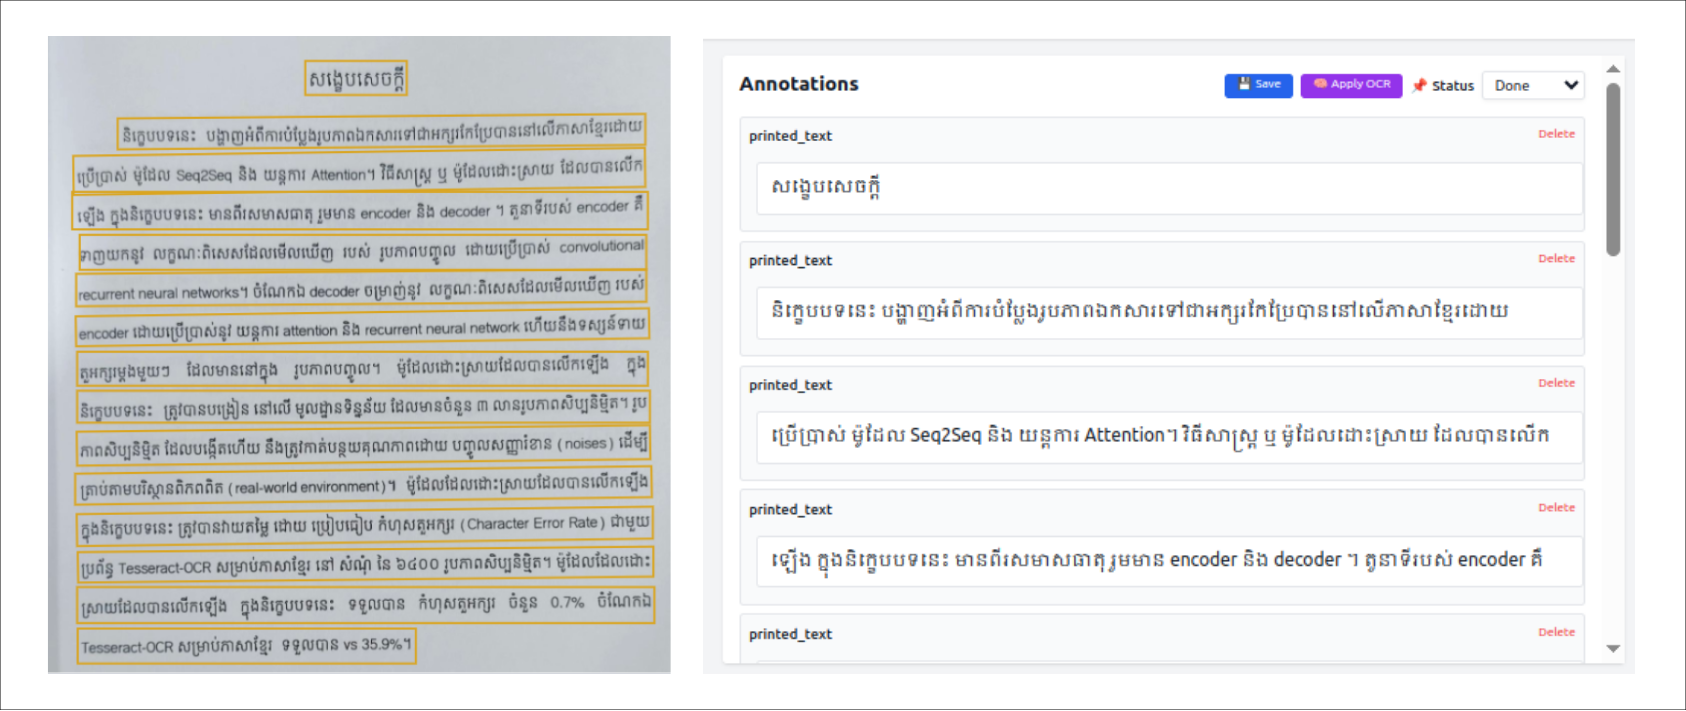
\includegraphics[width=\textwidth]{figures/craft_text_annotation.png}
    \caption{\englishfont The example of text detection dataset collection using commercial API}
    \label{fig:data_craft_collection}
\end{figure}


{\englishfont This hybrid approach significantly 
reduced annotation time while ensuring the final dataset quality met our standards.
The entire data collection and annotation process was facilitated by a custom-built 
annotation tool developed specifically for this project. This tool was designed with 
easy integration capabilities for commercial APIs, allowing seamless incorporation of 
automated suggestions while providing intuitive interfaces for manual correction 
and refinement. The tool's flexible architecture enabled rapid switching between 
different API providers and manual annotation modes, optimizing the overall annotation 
workflow.
Throughout the training process, a variety of data augmentation techniques were 
employed to enhance the model's robustness against font diversity, image noise, 
and other real-world distortions.

These transformations enriched the training set with diverse visual variations, 
which helped the model generalize more effectively to unseen data. The final 
manually annotated dataset comprised 7000 high-quality bounding boxes that captured 
the intricate structure of the Khmer script, ensuring robust training data for the 
CRAFT model fine-tuning process. }



\subsection{CRAFT Training Experiment}
\label{subsec:craft-training-results}

{\englishfont
The CRAFT model was evaluated during training using precision, recall, and Intersection over
Union (IoU) metrics. The text detection model demonstrated excellent performance in detecting text 
regions with high accuracy as you can see in the Figure~\ref{fig:iou-recall-craft}.
}
 
\begin{figure}[H]
    \centering
    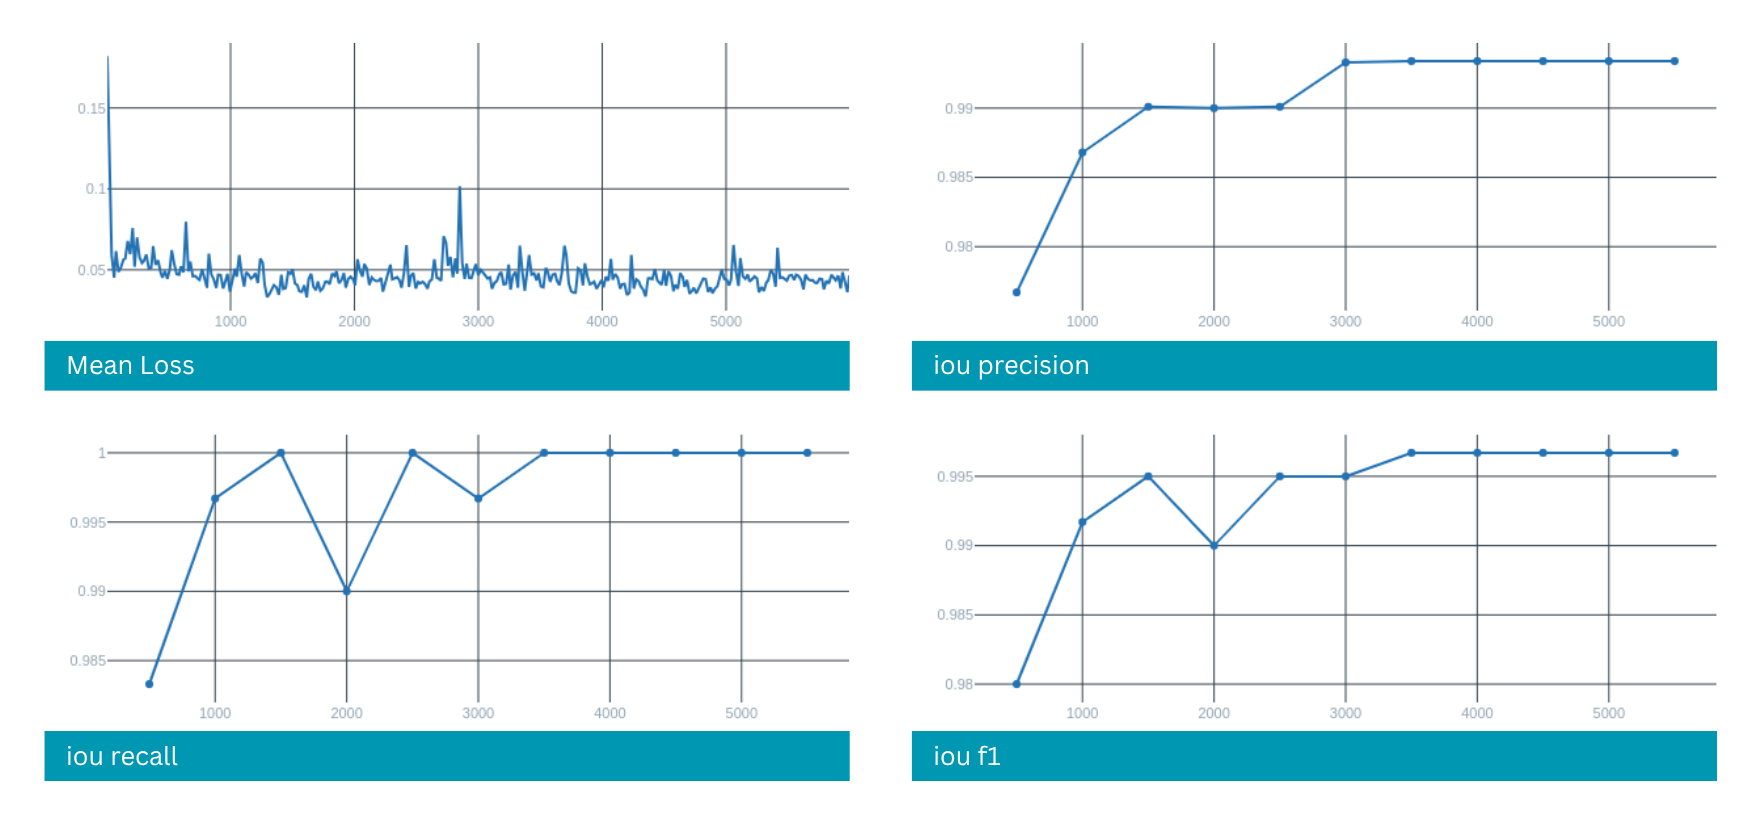
\includegraphics[width=\textwidth]{figures/craft_traning_process_5000.png}
    \caption{Illustration of the recall, precision, and the intersection over union 
    (IOU) performance of the CRAFT model with 5000 steps.}
    \label{fig:iou-recall-craft}
\end{figure}



\section{TrOCR for Text Recognition}
\label{sec:trocr-complete}

This section provides a comprehensive examination of the TrOCR (Transformer-based Optical Character Recognition) model implementation, including its architecture, customization for Khmer script, training methodology, and evaluation results.

\subsection{TrOCR Model Architecture}   
\label{subsec:trocr-architecture-architecture}

For the text recognition component of the pipeline, we used the \textbf{TrOCR} model, a transformer-based OCR system proposed by Microsoft Research. TrOCR stands for \textit{Transformer-based Optical Character Recognition}, and it integrates a vision encoder with a language decoder in a unified encoder-decoder (Seq2Seq) architecture, following the structure of the Vision Transformer (ViT) and pre-trained language models like BART.

The TrOCR model takes the cropped text-line image detected by CRAFT and processes it through a \textbf{ViT-based encoder}, which extracts rich visual features. These features are then passed to the \textbf{transformer decoder}, which generates the text sequence token-by-token, using cross-attention to focus on relevant image features while decoding. This allows the model to handle complex scripts like Khmer with better accuracy and context-awareness.

\begin{figure}[H]
    \centering
    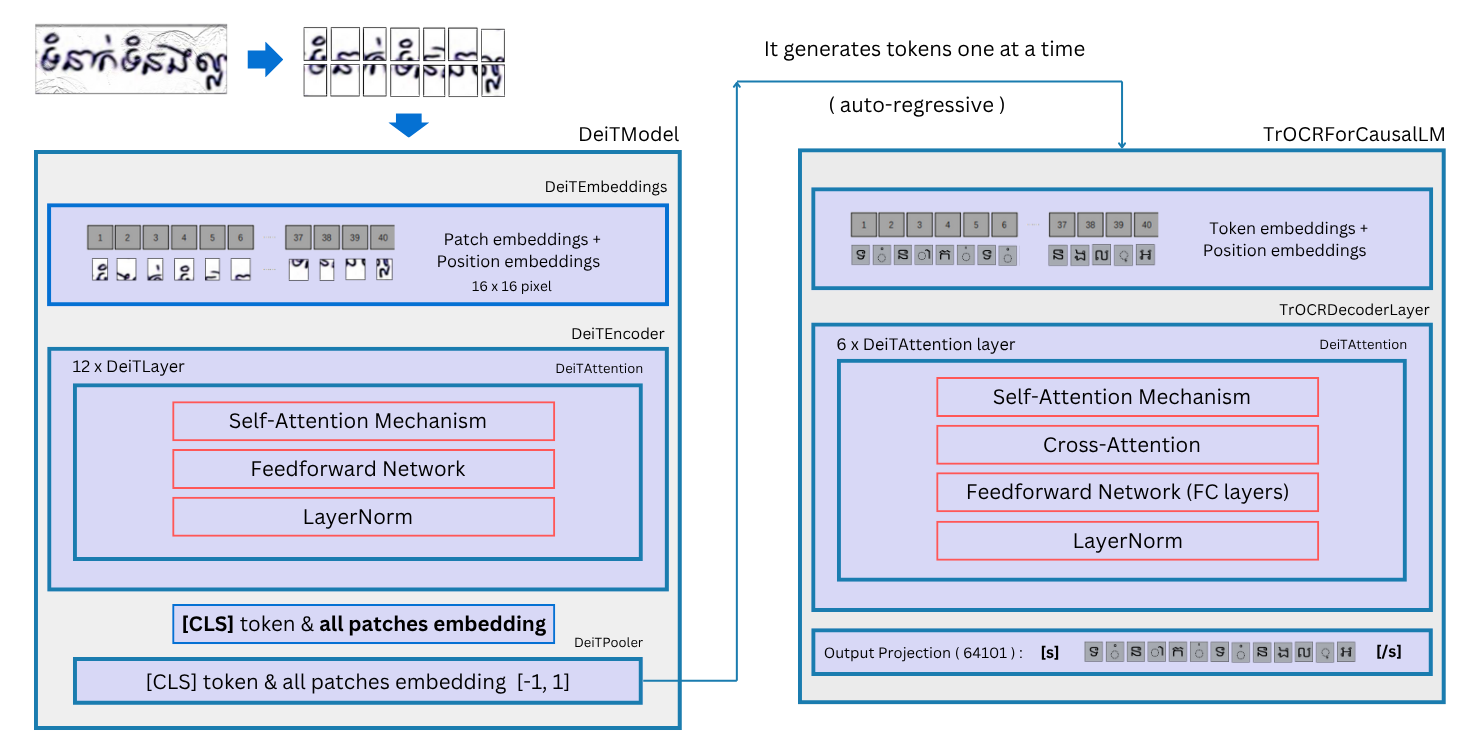
\includegraphics[width=\textwidth]{figures/trocr_model.png}
    \caption{Illustration of the TrOCR model architecture used for text recognition.}
    \label{fig:trocr-model}
\end{figure}


\subsection{Architecture Overview}
\label{subsec:trocr-architecture-overview}  

The TrOCR architecture consists of two main components~\cite{li2021trocr}:

\begin{itemize}
    \item \textbf{Vision Encoder:} A pre-trained Vision Transformer (ViT)~\cite{dosovitskiy2020image}, which
     extracts a sequence of visual features from input images.
    \item \textbf{Text Decoder:} A GPT-2-style autoregressive transformer that 
    generates character sequences from the visual features \cite{li2021trocr}.
\end{itemize}

Let the input image be denoted as $I \in \mathbb{R}^{H \times W \times 3}$.

\subsubsection*{Encoder: Vision Transformer}

The image $I$ is split into a sequence of $N$ patches, each of size $P \times P$. 
These patches are linearly projected into embeddings and processed through a Transformer encoder:

\[
x_0 = [\text{CLS}; x^1; x^2; \dots; x^N] + E_{pos}
\]

\[
Z = \text{TransformerEncoder}(x_0)
\]

where $x^i$ is the $i$-th patch embedding, $E_{pos}$ is the 
positional encoding, and $Z \in \mathbb{R}^{N \times D}$ is the final visual 
feature representation of the image.

\subsubsection*{Decoder: Autoregressive Transformer}

The decoder takes the encoder's output $Z$ and generates a 
character sequence $y = (y_1, y_2, \dots, y_T)$:

\[
P(y_t | y_{<t}, Z) = \text{softmax}(W_o h_t)
\]

\[
h_t = \text{DecoderBlock}(y_{<t}, Z)
\]

where $W_o$ is the output projection matrix and $h_t$ is the hidden state at time step $t$.




\subsection{Custom TrOCR Processor for Interpretability on Khmer}
\label{subsec:trocr-customization}

To make the TrOCR model understand Khmer tokens, we customized the processor without modifying the original model architecture. We developed a CustomKhmerTokenizer based on a predefined list of unique Khmer and English characters, including special tokens such as \textit{<s>}, \textit{</s>}, and \textit{<pad>}, to handle the encoding of text into token IDs and the decoding of token IDs back into readable text.

This tokenizer was then wrapped inside a custom processor that mimics the behavior of Hugging Face's TrOCRProcessor, allowing seamless integration with TrOCR's image processing pipeline. By doing so, we enabled the model to work with Khmer script during both training and inference, while preserving the original TrOCR model's structure and leveraging its pretrained capabilities.

\begin{figure}[H]
    \centering
    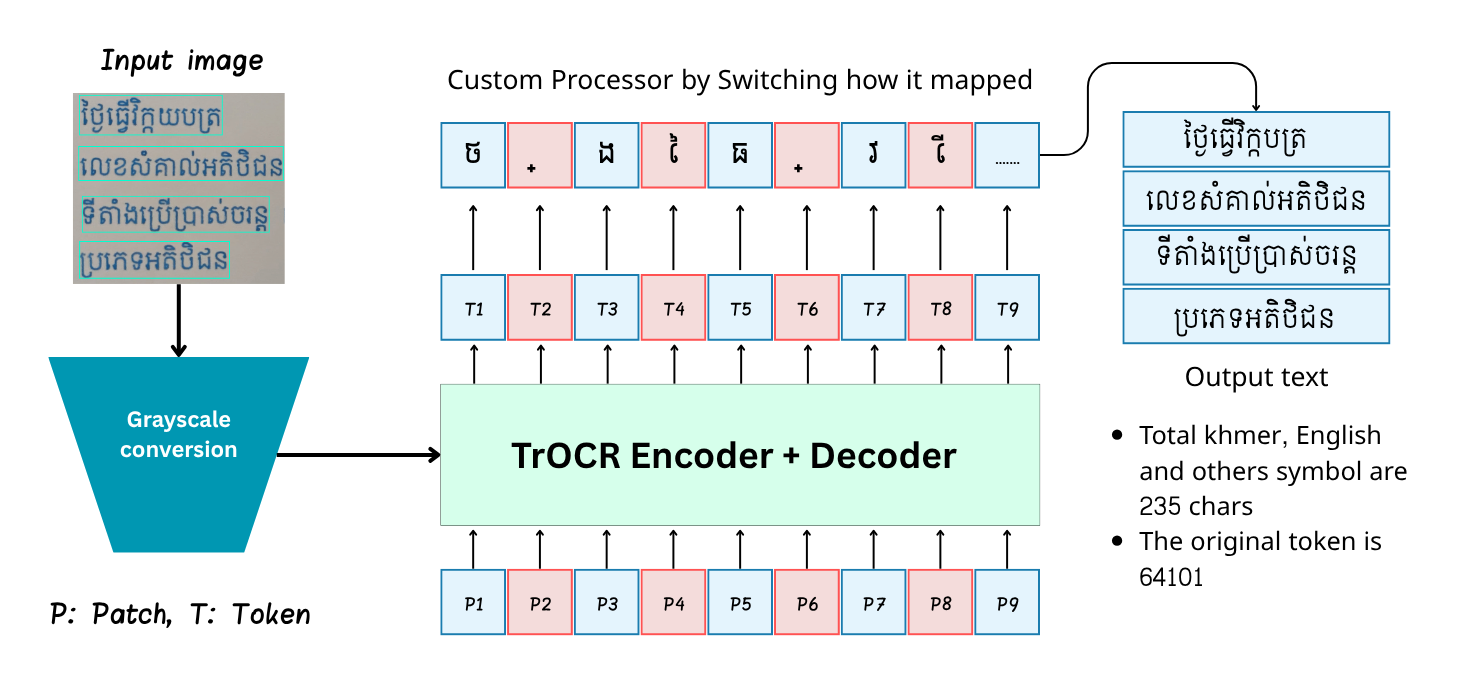
\includegraphics[width=\textwidth]{figures/Customize_processor.png}
    \caption{Architecture of the customized TrOCR pipeline. 
    The original TrOCR model is extended with a custom processor, 
    which is tailored for Khmer character decoding.}
    \label{fig:trocr-custom-processor}
\end{figure}

\subsection{Training TrOCR Workflow}
\label{subsec:trocr-training}

For the TrOCR model, we selected the base model because we were working with a multilingual dataset and wanted the model to have sufficient parameter capacity for this task. The training dataset consisted of 7.4 million synthetic images generated using our text-to-image pipeline.

\begin{figure}[H]
    \centering
    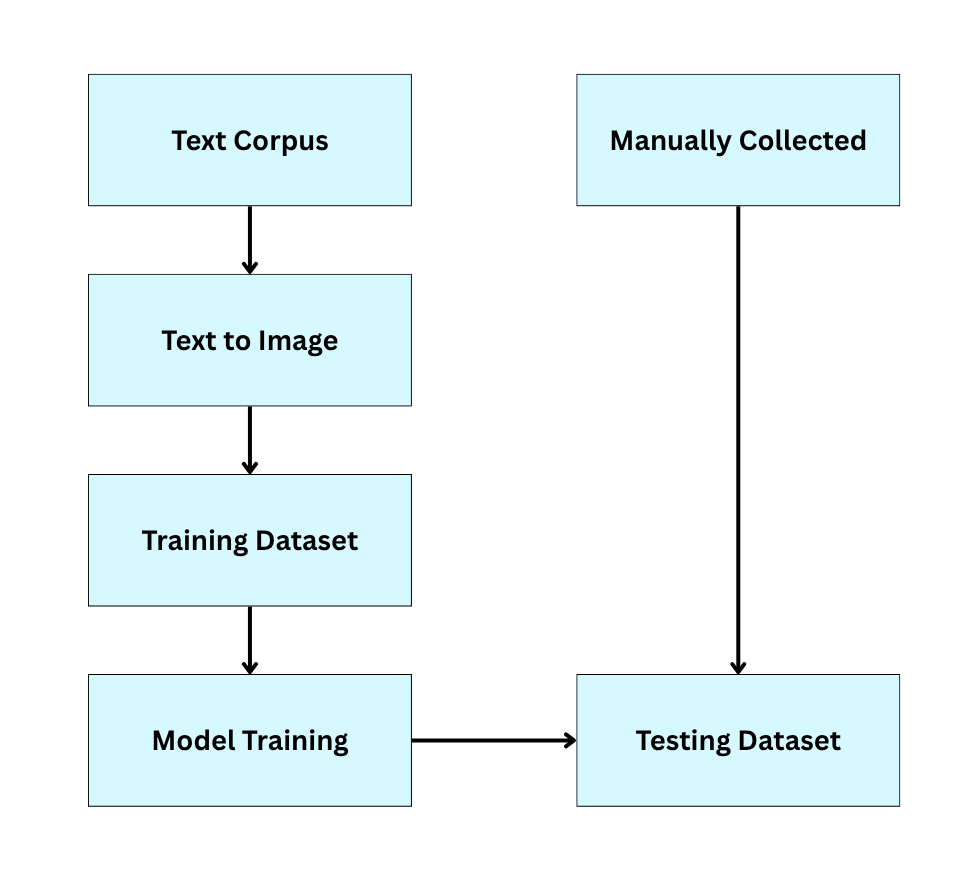
\includegraphics[width=\textwidth]{figures/trocr_model_overflow_training.png}
    \caption{Overview of the TrOCR training process. Text-generated 
    images form the training set, while real-world samples are 
    manually collected for testing and evaluation.}
    \label{fig:trocr-training-pipeline}
\end{figure}

The choice of batch size 1024 was crucial for model generalization. Initial experiments with smaller batch sizes (8, 16, 32, 128, 256) resulted in severe overfitting, as demonstrated in Figure~\ref{fig:trocr-overfitting}.

\subsection{TrOCR Training Results and Performance}
\label{subsec:trocr-training-results}

After experimenting with different hyperparameters, we found the optimal configuration:
\begin{itemize}
\item \textbf{Batch size}: 1024
\item \textbf{Learning rate}: 0.00001
\item \textbf{Epochs}: 3
\item \textbf{Dataset size}: 7.4 million images
\end{itemize}


\begin{figure}[H]
    \centering
    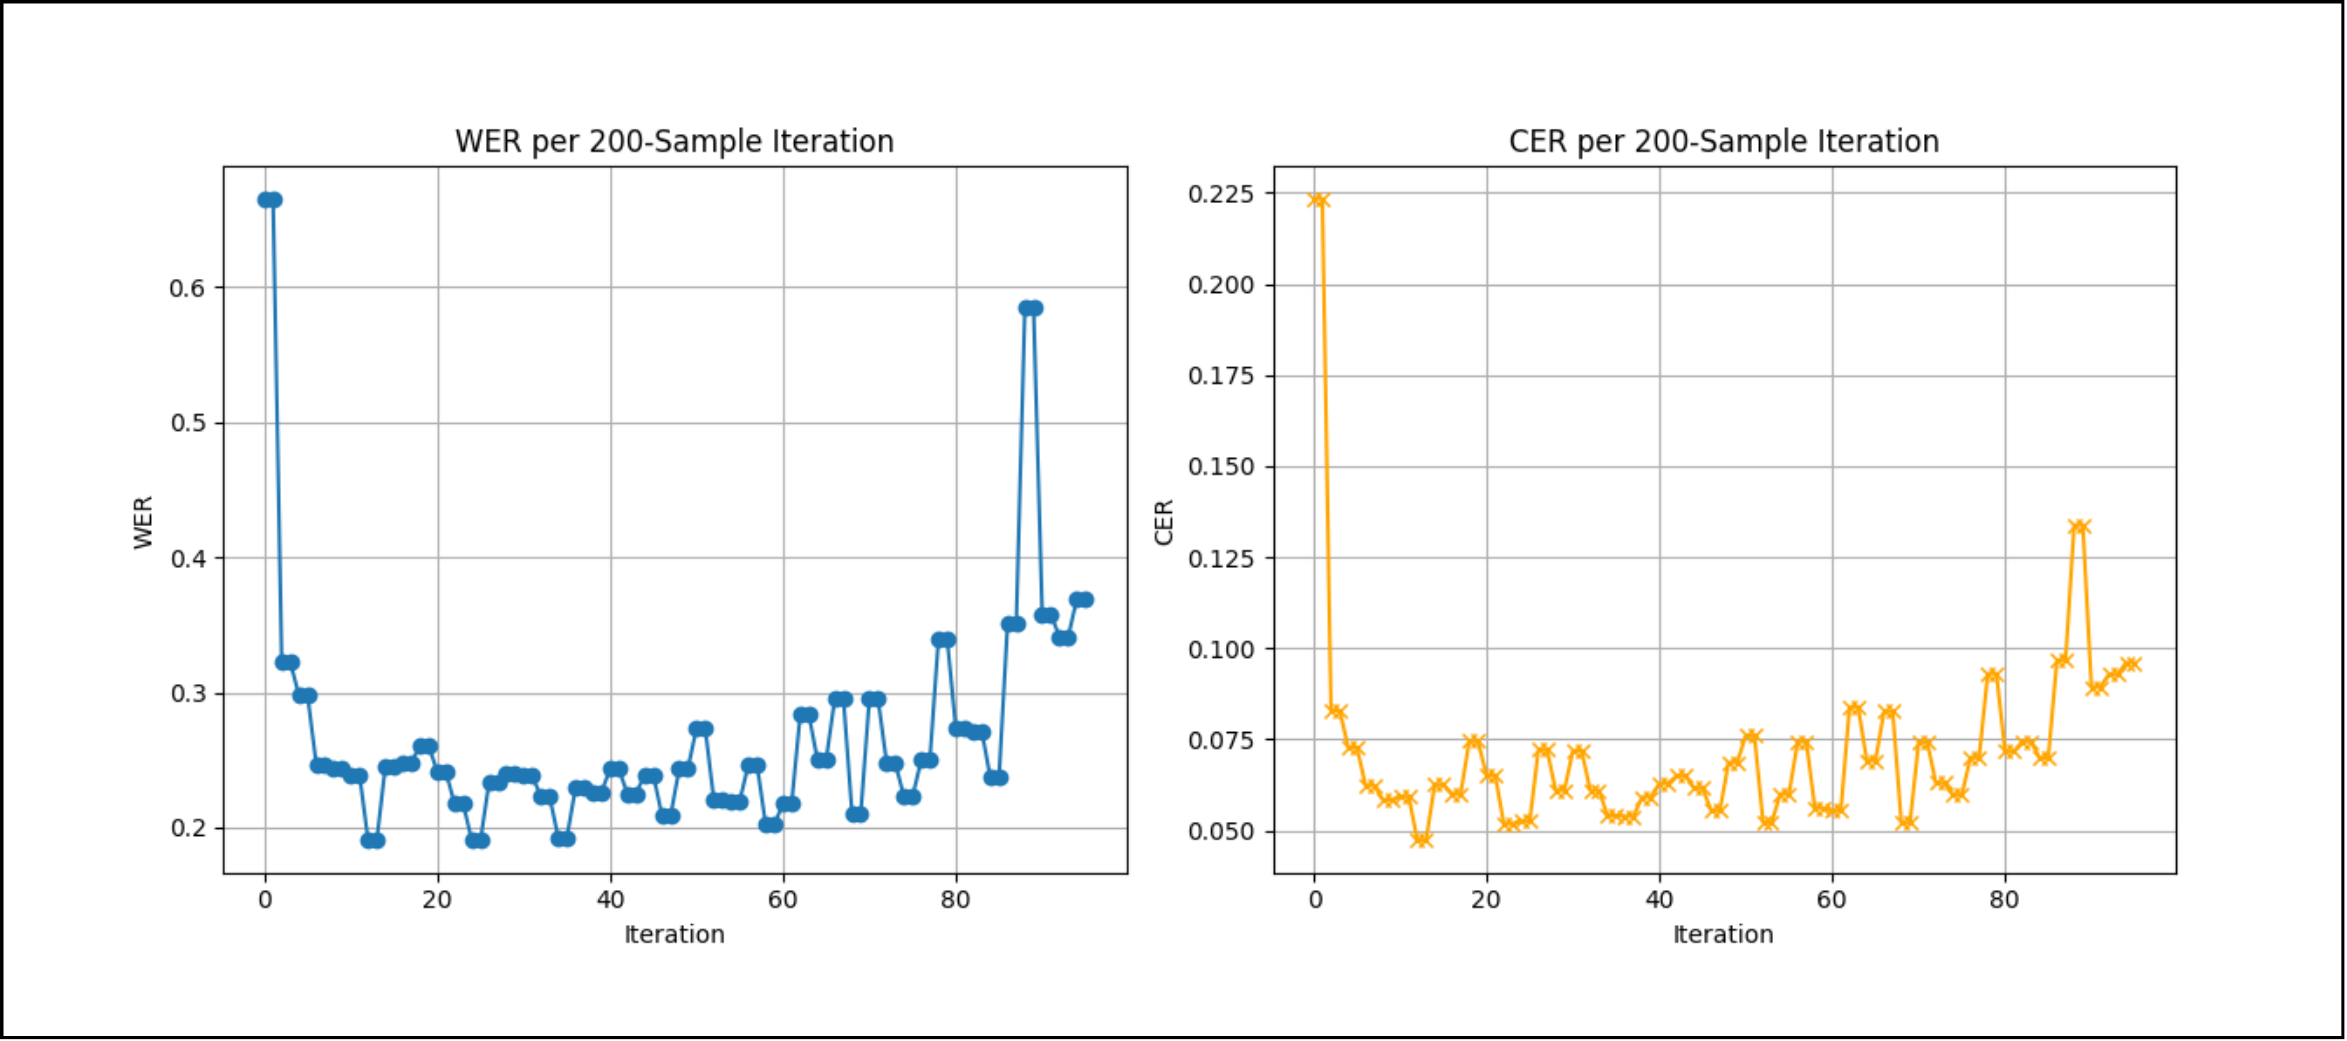
\includegraphics[width=\textwidth]{figures/trocr_overfitting_v1.png}
    \caption{Training and validation loss curves for TrOCR model with batch size 8, 
    clearly showing overfitting behavior where training loss decreases while validation loss increases.}
    \label{fig:trocr-overfitting}
\end{figure}

The graph above illustrates a clear case of overfitting when using a batch size of 8. The training loss continues to decrease while the validation loss starts to increase, indicating that the model learns very specific patterns from the training data rather than generalizing well to unseen data.

\begin{figure}[H]
    \centering
    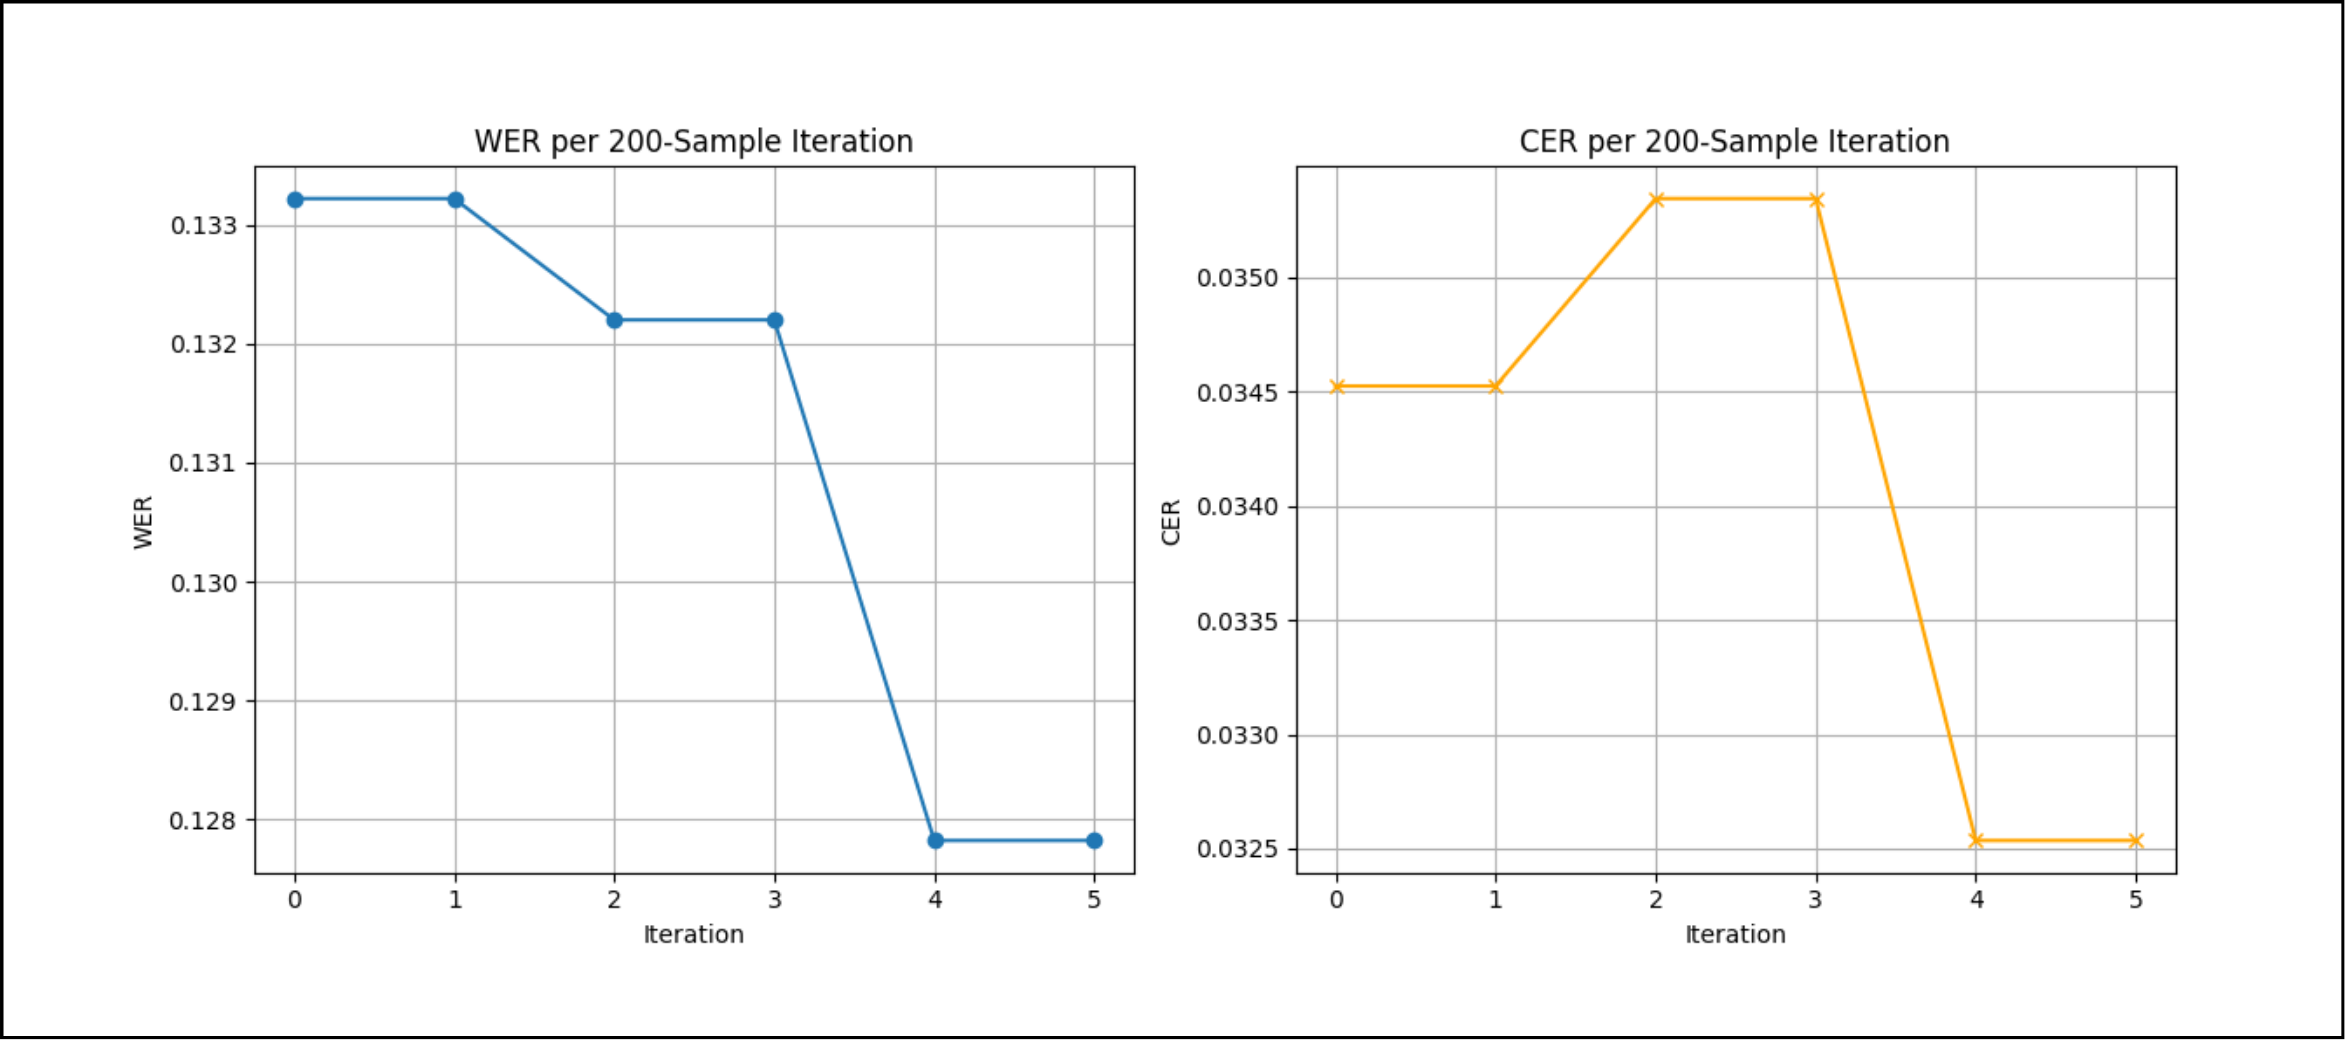
\includegraphics[width=\textwidth]{figures/trocr_fine_tuning.png}
    \caption{Training and validation metrics for TrOCR model with batch size 1024, 
    showing Character Error Rate (CER) and Word Error Rate (WER) over training steps. 
    The model demonstrates excellent performance from early training steps, with CER quickly 
    reaching around 0.03 and WER staying below 0.12.}
    \label{fig:trocr-fine-tuning}
\end{figure}

With the optimized batch size of 1024, the model showed remarkable performance from early stages of training, with CER quickly stabilizing around 0.03 and WER maintaining values below 0.12. This rapid convergence can be attributed to the utilization of pretrained weights and the larger batch size enabling better generalization.


\section{End-to-End OCR Pipeline}
\label{sec:end-to-end-pipeline}

This section describes the integration of CRAFT and TrOCR models into a unified end-to-end OCR system capable of processing multilingual documents containing both Khmer and English text.

\subsection{Pipeline Architecture}
\label{subsec:pipeline-architecture}

The overall workflow is presented in Figure~\ref{fig:trocr-inference-full-pipeline}. The pipeline begins with input images containing English and Khmer text, or mixed-language content. The preprocessing step converts images to grayscale to streamline downstream processing and improve model prediction accuracy.

\begin{figure}[H]
    \centering
    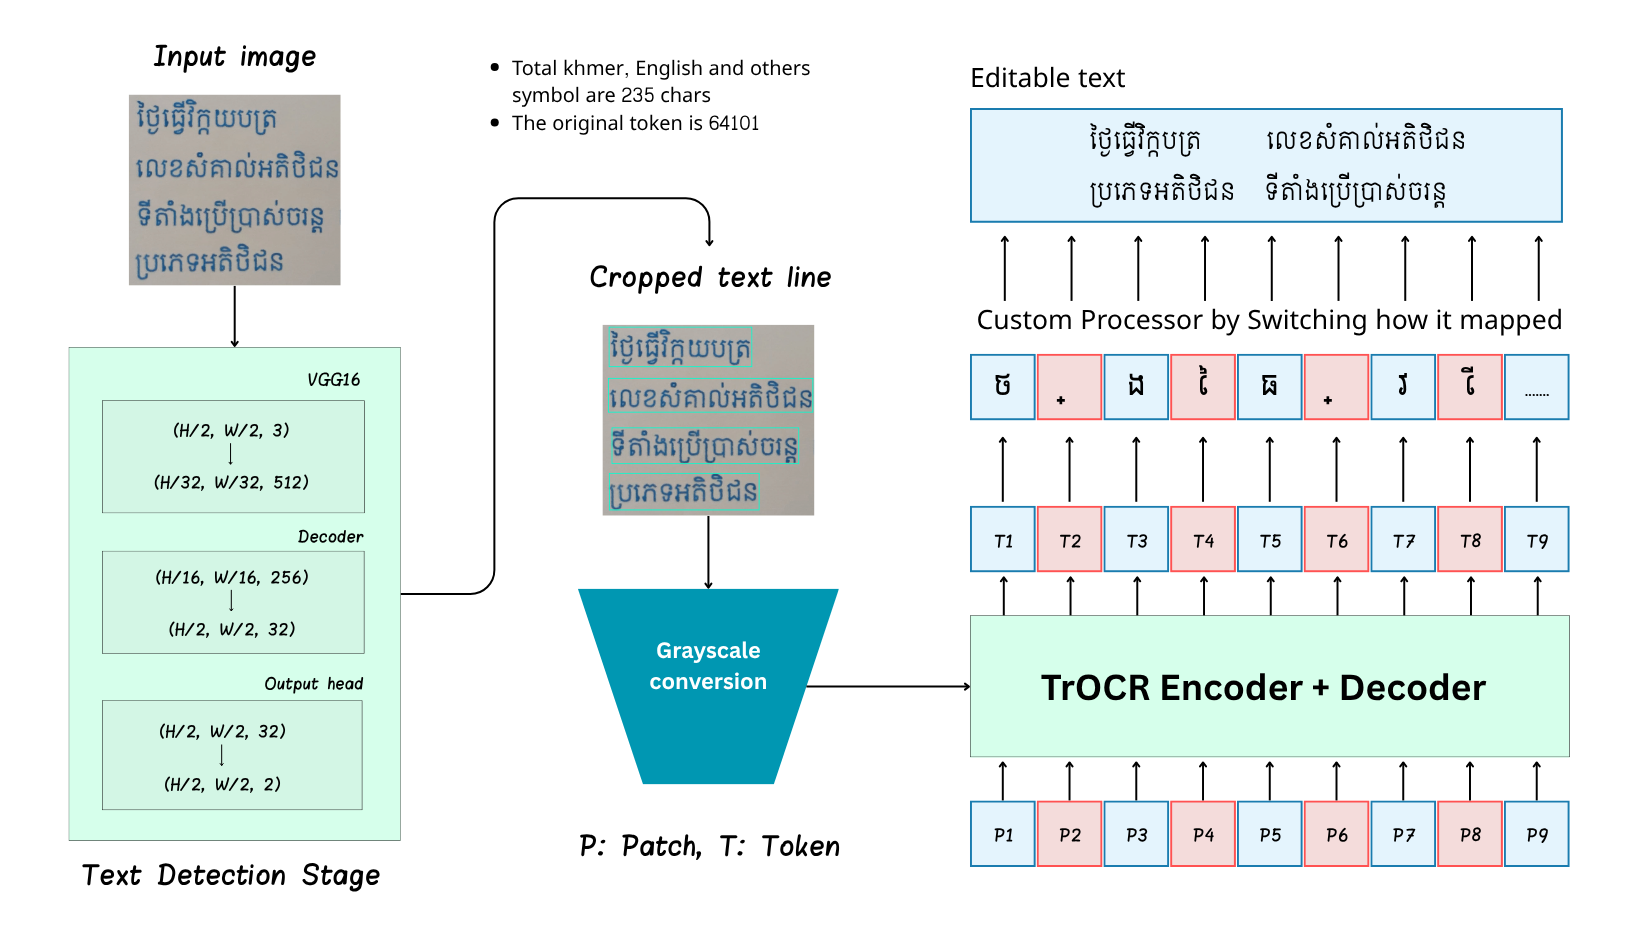
\includegraphics[width=\textwidth]{figures/khmerOCR_inference_full_pipeline.png}
    \caption{End-to-end OCR inference pipeline for converting text images into digital text.}
    \label{fig:trocr-inference-full-pipeline}
\end{figure}

\subsection{Pipeline Processing Steps}
\label{subsec:pipeline-steps}

The complete pipeline operates through the following sequential steps:

\begin{enumerate}
\item \textbf{Image Preprocessing}: Input images are converted to grayscale and normalized to ensure consistent processing across different image types and qualities.

\item \textbf{Text Detection}: The CRAFT model detects text regions in the image on a text-line basis, generating bounding boxes for each detected text segment.

\item \textbf{Post-processing and Reordering}: Detected text-lines undergo post-processing to ensure correct reading order, accounting for document layout and text flow patterns.

\item \textbf{Text-line Cropping}: Individual text-line regions are extracted from the original image based on CRAFT detection results.

\item \textbf{Text Recognition}: Each cropped text-line image is processed by the TrOCR model to generate the corresponding digital text output.

\item \textbf{Output Assembly}: Recognized text from all text-lines is assembled in the correct order to produce the final digital document.
\end{enumerate}

\subsection{Pipeline Integration Benefits}
\label{subsec:pipeline-benefits}

The integration of CRAFT and TrOCR provides several advantages:

\begin{itemize}
\item \textbf{Character-level Detection}: CRAFT's character-aware detection is particularly effective for complex scripts like Khmer with stacked characters and diacritics.

\item \textbf{Transformer-based Recognition}: TrOCR's attention mechanism allows for better context understanding and improved accuracy on both Khmer and English text.

\item \textbf{Multilingual Support}: The pipeline seamlessly handles documents containing both Khmer and English text without requiring language-specific preprocessing.

\item \textbf{End-to-end Processing}: The unified pipeline eliminates the need for manual intervention between detection and recognition stages.
\end{itemize}

This comprehensive approach ensures robust performance across diverse document types and text conditions, making it suitable for real-world OCR applications in multilingual environments.

}
\chapter{Results and Analysis}
\phantomsection
\label{ch:results}

\vspace{-1cm}
\setlength{\parindent}{0pt}
\vspace{0.3cm}

\section{Text Detection Results}
\label{sec:detection-results}

{\englishfont\fontsize{13.5pt}{17pt}\selectfont

The text detection model, based on the CRAFT (Character Region Awareness for Text detection) 
architecture, was evaluated on a test set consisting of 60 images. The model achieved an impressive 
Intersection over Union (IoU) score of 0.85 when compared to the ground truth annotations, 
demonstrating high accuracy in detecting text regions.


The training process was conducted on a dataset of 369 images, with an additional 60 images 
used for validation. The evaluation results indicate that the model is capable of accurately 
detecting text in all test images, showcasing its generalization ability and robustness across 
various text-containing scenes.

\begin{figure}[H]
    \centering
    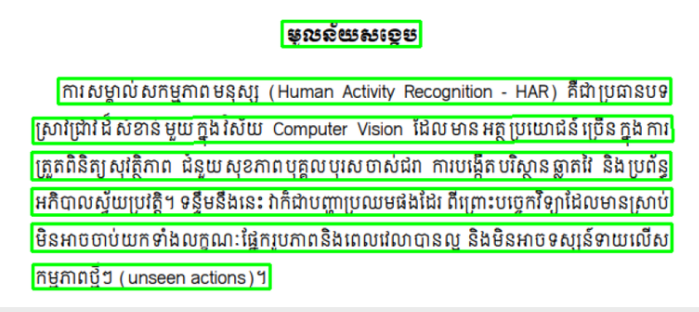
\includegraphics[width=1\textwidth]{figures/image_detection_craft_01.png}
    \caption{Testing with documentation image type: example of text detection using the CRAFT 
    model on a natural scene text image.}
    \label{fig:detection-craft}
\end{figure}

The results from testing with clean text from documentation images are shown in Figure 
\ref{fig:detection-craft}. The model is able to detect text in each sentence, 
even when the text is separated by spaces. This is important for the OCR model to 
work with short text sentences, as it is able to recognize the text more accurately. 
For example, if the model is given the text "This is a test", it should be able to 
detect each word as a single entity, rather than as whole sentence. 
By detecting text in this way, the model is able to recognize the text 
more accurately.

\begin{figure}[H]
    \centering
    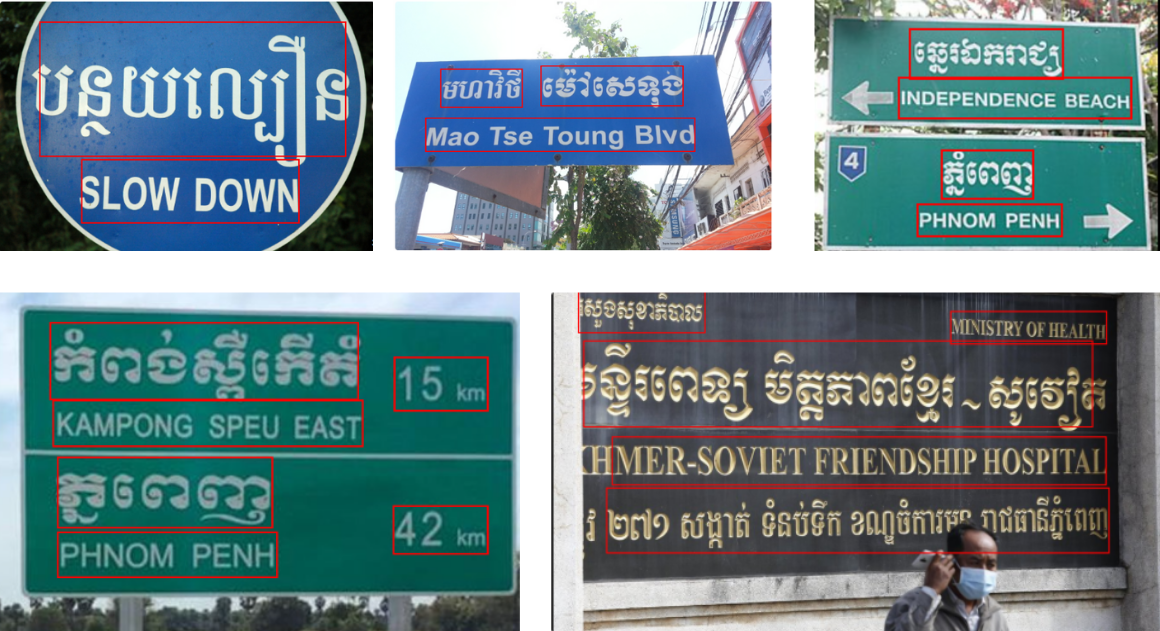
\includegraphics[width=1\textwidth]{figures/image_detection_craft_02.png}
    \caption{Example testing with image on the street and complex scenes: using the CRAFT 
    model on a natural scene text image.}
    \label{fig:detection-craft-post}
\end{figure}

\begin{figure}[H]
    \centering
    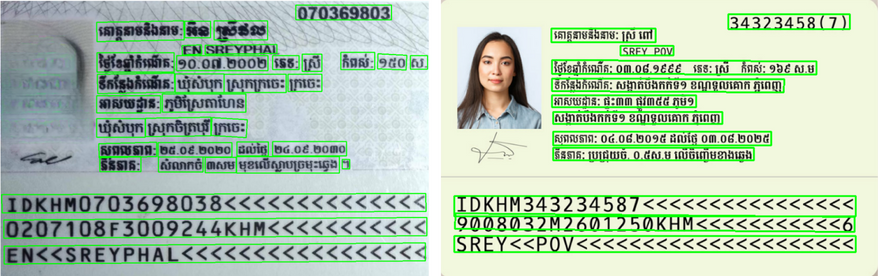
\includegraphics[width=1\textwidth]{figures/testing_with_khmer_id.png}
    \caption{Example testing Khmer ID Card image with CRAFT model.}
    \label{fig:detection-craft-post-with-khmer-id}
\end{figure}


As you can see from the example in Figure \ref{fig:detection-craft-post}, 
the model is able to detect text even when it is very small, such as the text on the poster. 
This demonstrates the model's robustness and ability to detect text in a variety of contexts and scenarios.



\subsection{CRAFT Evaluation Metrics}
\label{subsec:craft-evaluation}

The results presented in Table~\ref{tab:craft_experimental_result} are based on experiments 
conducted using a manually annotated dataset consisting of 60 images containing both Khmer and English 
text. To evaluate the performance of the text detection model, standard metrics were employed: 
Precision, Recall, F1-score (also referred to as H-Mean), and Intersection over Union (IoU). 
These metrics provide a comprehensive view of the model’s accuracy in identifying text regions. 
The table summarizes the outcomes under various combinations of Region Score threshold, 
Affinity Score threshold, Low Text threshold, and canvas size settings (denoted in the RALC column), 
reflecting the model's adaptability across different configurations.

\begin{table}[H]
    \centering
    \caption{Summary of Text Detection Results}
    \renewcommand{\arraystretch}{1.5}
    \begin{tabular}{|p{3.5cm}|p{3.0cm}|p{3.0cm}|p{2.0cm}|p{3.0cm}|}
    \hline
    \textbf{RALC} & \textbf{Avg Precision} & \textbf{Avg Recall} & \textbf{H-Mean} & \textbf{Avg IoU} \\
    \hline
    0.3,0.2,0.1,3240 & 0.3718 & 0.2296 & 0.2648 & 0.2404\\
    \hline
    0.5,0.4,0.4,3240 & 0.9628 & 0.9794 & 0.9680 & 0.8383\\
    \hline
    0.6,0.5,0.5,3240 & 0.9480 & 0.9702 & 0.9558 & 0.7431\\
    \hline
    0.7,0.7,0.4,3240 & 0.2909 & 0.4242 & 0.3350 & 0.2391\\
    \hline
    0.7,0.6,0.5,2440 & 0.7878 & 0.8798 & 0.8239 & 0.6039\\
    \hline
    0.6,0.6,0.5,3440 & 0.7527 & 0.8797 & 0.8025 & 0.5751\\
    \hline
    0.6,0.5,0.4,3240 & 0.9641 & 0.9805 & 0.9697 & 0.8363\\
    \hline
    0.7,0.5,0.4,2540 & 0.9792 & 0.9746 & 0.9751 & 0.8503\\
    \hline
    \end{tabular}
    \label{tab:craft_experimental_result}
\end{table}

{\englishfont Among all configurations, the best performance was achieved with RALC = 0.7, 0.5, 0.4, 2540, 
which yielded an F1-score of 0.9751 and an IoU of 0.8503. This indicates that this particular 
combination of Region Score = 0.7, Affinity Score = 0.5, Low Text = 0.4, and Canvas Size = 2540 
strikes an optimal balance between text detection sensitivity and bounding box precision. 
These results demonstrate that the model successfully adapted to Khmer script characteristics 
and can effectively detect text regions under diverse conditions.}

\subsection{Headmap Visualization}
\label{subsec:headmap_visualization}


\begin{figure}[H]
    \centering
    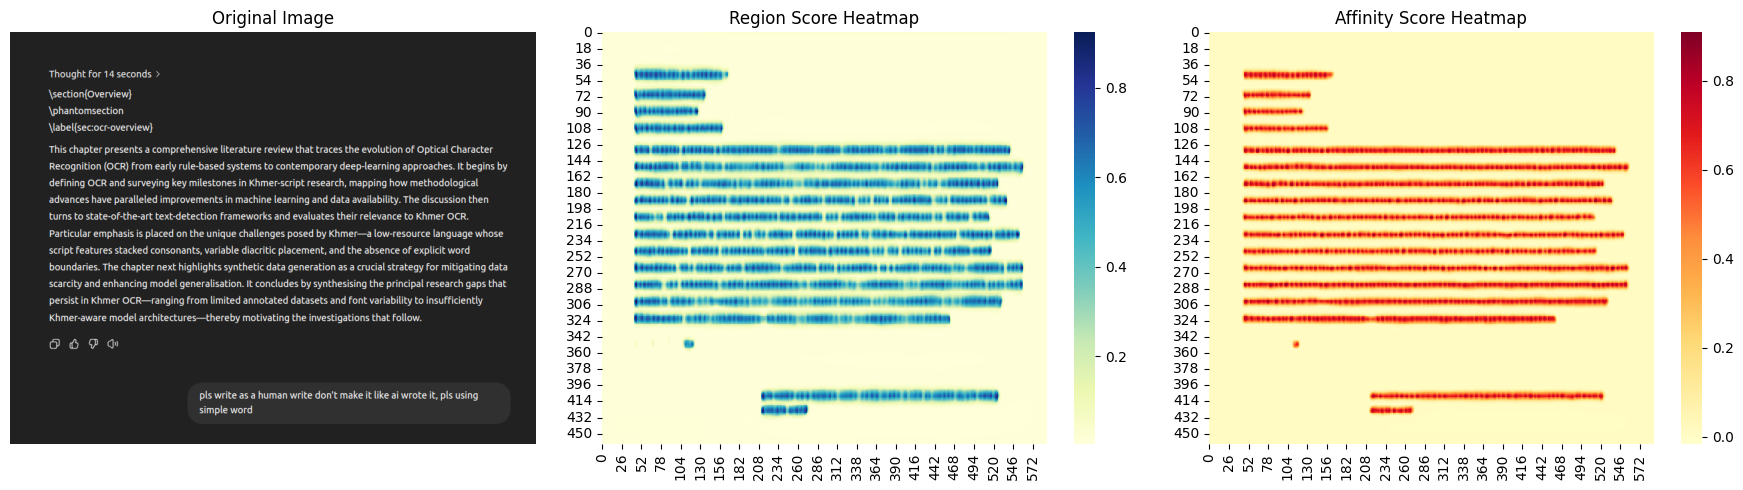
\includegraphics[width=\textwidth]{figures/Heatmap_visualization_craft.png}
    \caption{Headmap visualization of Region score and Affinity score of CRAFT model on English text.
    }
    \label{fig:headmap-craft-model-on-English}
\end{figure}

\begin{figure}[H]
    \centering
    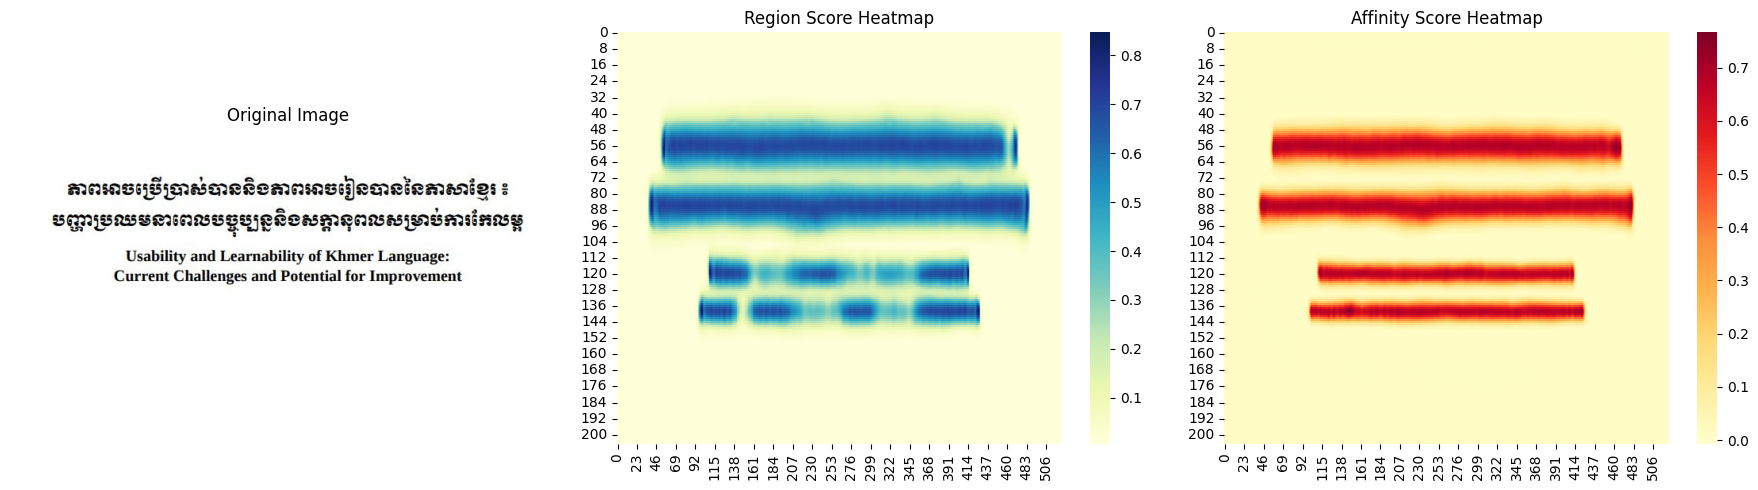
\includegraphics[width=\textwidth]{figures/Heatmap_visualization_craft_on_kh.png}
    \caption{Headmap visualization of Region score and Affinity score of CRAFT model on Khmer text.
    }
    \label{fig:headmap-craft-model-on-khmer}
\end{figure}



\section{Text Recognition Results}
\label{sec:recognition-results}
The text recognition model, based on the TrOCR (Transformer-based OCR) architecture, was
evaluated on a test set consisting of real dataset manually collected amount 7000 images, we
spend time around 10 days to collect this dataset for fairly evaluation. The testing dataset
containing such as char by char, word by word, and sentence by sentence, it's also included
both languages, Khmer and English. The model achieved an impressive result, we achieved CER
( Character Error Rate) of 0.12, demonstrating high accuracy
in recognizing text in the images.


\begin{figure}[H]
    \centering
    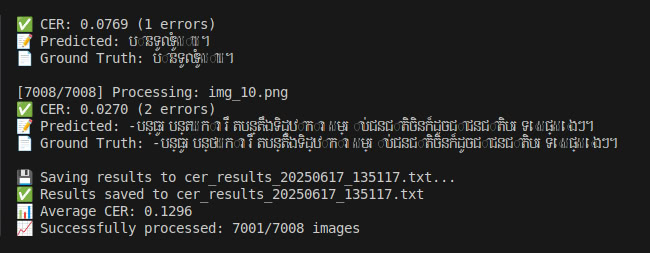
\includegraphics[width=\textwidth]{figures/result_log_trocr_with_7000_image.png}
    \caption{Testing Trocr model Evaluation Metrics by CER (Character Error Rate)}
    \label{fig:trocr_cer_log_result}
\end{figure}


\begin{figure}[H]
    \centering
    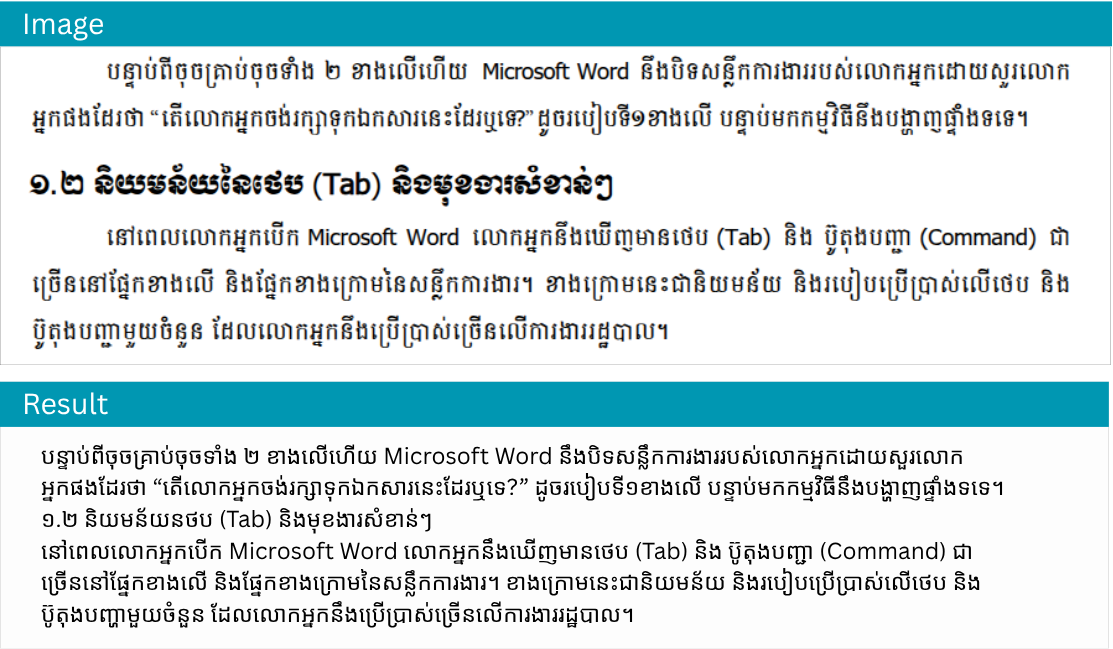
\includegraphics[width=\textwidth]{figures/result_image_to_text.png}
    \caption{End-to-end OCR result: The pipeline takes a raw image as input 
    and outputs recognized text directly without any manual preprocessing.}
    \label{fig:result_converted}
\end{figure}

\section{Error Analysis and Failure Cases}
\label{sec:error-analysis}
Our analysis revealed several cases where the model struggled to perform effectively. The primary failure cases can be categorized into two main scenarios:

1. Curved and Circular Text: The model encountered difficulties with text arranged in curved or circular patterns, as shown in Figure \ref{fig:test-case}. These cases proved challenging due to the complex spatial relationships between characters that deviate significantly from standard linear text layouts.

2. Non-standard and Artistic Text: Another significant challenge was presented by text written in unusual fonts and artistic styles. The text detection model particularly struggled with these cases, as the unconventional character shapes and varying sizes created complex visual patterns that were difficult for the model to process accurately.

\begin{figure}[H]
    \centering
    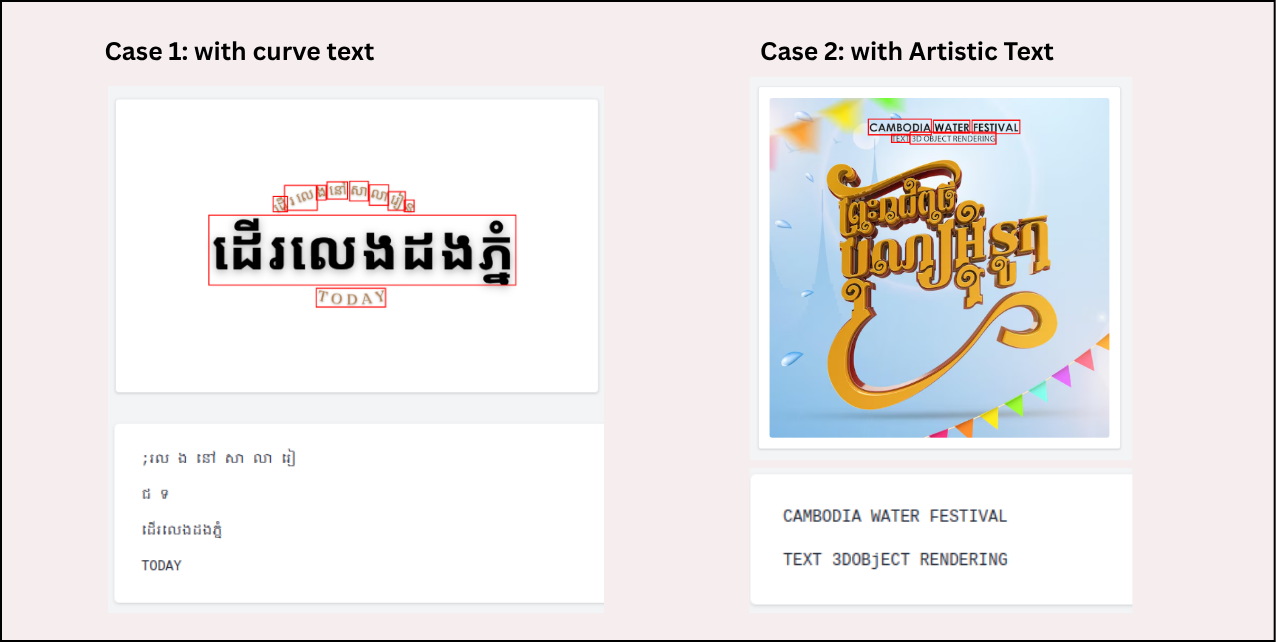
\includegraphics[width=\textwidth]{figures/test_case.png}
    \caption{Challenging cases involving both curved text layouts and artistic typography. 
    The model's performance degraded significantly when processing text arranged in circular 
    patterns and non-standard fonts, highlighting limitations in handling complex spatial 
    text arrangements and artistic text styles.}
    \label{fig:test-case}
\end{figure}

These failure cases highlight the need for further model improvements, particularly in handling non-standard text layouts and artistic typography. Future work could focus on enhancing the model's ability to process curved text and adapt to various artistic text styles.

\section{System Robustness and Generalization}
\label{sec:robustness}
The robustness and generalization capabilities of our text recognition model have demonstrated 
remarkable performance beyond our initial expectations. Despite being trained on a limited 
dataset of diversity fonts, the model exhibited impressive adaptability by 
successfully recognizing real-scene text, on documentation with different font styles. This significant 
improvement in font recognition capability highlights the model's strong generalization 
abilities, particularly when dealing with fonts that maintain similar structural characteristics 
to the training data.

A particularly noteworthy aspect of the model's robustness is its ability to handle slightly 
curved text. As demonstrated in our test cases, while the model struggles with severely 
curved or circular text arrangements (as shown in Figure \ref{fig:test-case}), it maintains 
high accuracy when processing text with moderate curvature. For instance, the model 
successfully recognized the word "TODAY" despite its slight curvature, showcasing 
its ability to handle non-linear text layouts within reasonable bounds.

This performance demonstrates that our model has developed a robust understanding of text 
features that transcends the specific characteristics of the training data. The model's 
ability to generalize to new font styles and handle moderate text curvature while 
maintaining high recognition accuracy validates the effectiveness of our approach 
and the model's practical applicability in real-world scenarios.
\section{Model Interpretability and Attention Visualization}
\label{sec:interpretability}

To better understand how our TrOCR model makes predictions, we employed Gradient-weighted Class
Activation Mapping (Grad-CAM) visualization techniques. Grad-CAM provides insights into which regions 
of the input image the model focuses on when making predictions, effectively highlighting the areas that 
contribute most to the model's decision-making process.

\begin{figure}[H]
    \centering
    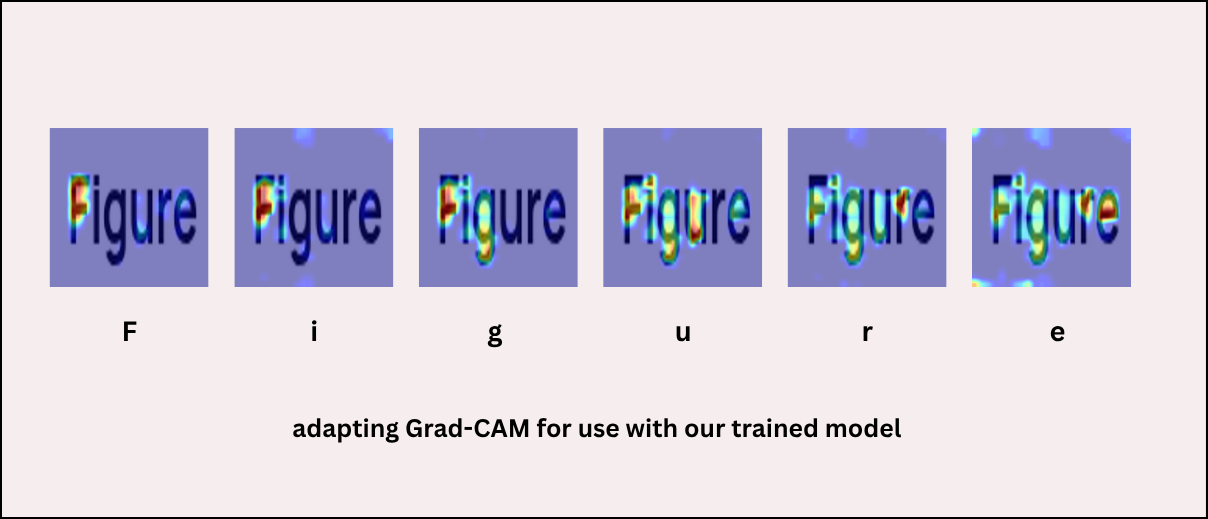
\includegraphics[width=\textwidth]{figures/grad_cam_figure.png}
    \caption{Grad-CAM visualization of the TrOCR model's attention on input text. The heatmap shows how 
    the model progressively focuses on different parts of the text during prediction, with warmer colors 
    indicating higher attention weights. This visualization reveals the model's systematic approach to text 
    recognition, starting from the beginning of the text and moving sequentially.}
    \label{fig:grad-cam-trocr}
\end{figure}

As shown in Figure \ref{fig:grad-cam-trocr}, the Grad-CAM visualization reveals several interesting patterns in the model's 
attention mechanism:

\begin{enumerate}
    \item Sequential Processing: The model demonstrates a clear left-to-right reading pattern, focusing attention 
    on one character or word at a time, which aligns with the natural reading order of text.
    
    \item Contextual Awareness: The attention maps show that the model considers surrounding characters when 
    making predictions, indicating its ability to understand contextual relationships between characters.
    
    \item Focus Intensity: The intensity of the attention (shown by the color gradient) varies based on the 
    complexity of the character or word being processed, with more complex characters receiving stronger attention.
\end{enumerate}

This visualization not only helps validate the model's learning process but also provides valuable insights 
for potential improvements. The clear sequential attention pattern suggests that the model has successfully 
learned the fundamental structure of text recognition, while the contextual awareness indicates its ability to 
handle the complex relationships between characters in Khmer script.

}
\chapter{API Development}
\phantomsection
\label{ch:development}

{\englishfont\fontsize{13.5pt}{17pt}\selectfont

\vspace{-1cm}
\setlength{\parindent}{0pt}
\vspace{0.3cm}

\section{Introduction to API Development}
\label{sec:api-introduction}

The transition from research prototype to production-ready system represents a critical phase in making OCR technology accessible to real-world applications. While many academic research projects remain confined to laboratory settings, this work aims to bridge the gap between theoretical advancement and practical deployment. By developing a robust API (Application Programming Interface) for our Khmer-English OCR system, we enable seamless integration into various applications, from mobile apps to web services and enterprise systems.

The development of this API serves multiple purposes: it validates the practical utility of our research findings, provides a standardized interface for accessing OCR capabilities, and creates a foundation for broader adoption of Khmer text processing technology. This chapter details the architectural decisions, implementation challenges, and deployment strategies that transform our research models into a production-ready service.

\section{System Architecture Overview}
\label{sec:system-architecture}

\subsection{Microservices Architecture}
\label{subsec:microservices}

Our API implementation follows a microservices architecture pattern, separating the text detection and text recognition components into distinct, scalable services. This design choice offers several advantages:

\begin{itemize}
\item \textbf{Independent scaling}: Text detection and recognition services can be scaled independently based on demand
\item \textbf{Fault isolation}: Issues in one service don't affect the entire system. However, if one system down the another system can't be work alone, but following this way it's easily for debugging and update the issues.
\item \textbf{Technology flexibility}: Each service can be optimized with different frameworks and configurations
\end{itemize}

\subsection{Service Components}
\label{subsec:service-components}

The API architecture consists of two primary components:

\begin{enumerate}
\item \textbf{CRAFT Text Detection Service}: Implements the CRAFT model for identifying text regions in images.
\item \textbf{TrOCR Text Recognition Service}: Utilizes the customized TrOCR model for converting detected text regions into digital text
\end{enumerate}

\subsection{Data Flow Pipeline}
\label{subsec:data-flow}

The complete OCR pipeline processes requests through the following stages:

\begin{enumerate}
\item \textbf{Image Reception}: Services receive image data via HTTP POST requests
\item \textbf{Preprocessing}: Images are validated, normalized, and prepared for processing
\item \textbf{Text Detection}: The CRAFT service identifies and extracts text-line bounding boxes
\item \textbf{Region Extraction}: Individual text regions are cropped based on detection results
\item \textbf{Text Recognition}: Each text region is processed by the TrOCR service
\item \textbf{Post-processing}: Results are assembled, ordered, and formatted for response
\item \textbf{Response Delivery}: Final OCR results are returned to the client
\end{enumerate}

\section{CRAFT Text Detection API Service}
\label{sec:craft-api}

\subsection{Service Implementation}
\label{subsec:craft-implementation}

The CRAFT text detection service is implemented using FastAPI, a modern Python web framework chosen for its automatic API documentation generation, built-in data validation, and high performance. The service runs on GPU-enabled containers with NVIDIA CUDA support.

\subsubsection*{Main Application Structure}

\begin{verbatim}
def main():
    # FastAPI app initialization
    app = FastAPI(title="CRAFT Text Detection API")

    # CORS middleware setup
    # Model loading and GPU configuration
    # API endpoint definitions

def load_model(model_path, device):
    # Load CRAFT model from checkpoint
    # Apply state dict and move to GPU
    # Set model to evaluation mode

def predict_endpoint(file):
    # Save uploaded image temporarily
    # Convert image format (BGR or RGB to Grayscale Color)
    # Run CRAFT inference
    # Apply bounding box adjustments
    # Format and return results
    # Clean up temporary files

\end{verbatim}

\subsubsection*{Input and Output Specifications}

\textbf{Input Requirements:}
\begin{itemize}
\item \textbf{Endpoint}: \texttt{POST /predict}
\item \textbf{Input}: Image file (JPEG, PNG, supported formats)
\item \textbf{File size}: Recommended under 3MB for optimal performance
\item \textbf{Image format}: Automatically converted to RGB format internally
\end{itemize}

\textbf{Output Format:}
The service API returns as JSON responses with detected text regions as 4-point polygons that is easily for passing to another pipeline:

    \begin{verbatim}
    {
    "boxes": [
        {
        "box": [
            [x1, y1], [x2, y2], [x3, y3], [x4, y4]
        ]
        }
    ]
    }
    \end{verbatim}

\subsection{Model Configuration and Optimization}
\label{subsec:craft-config}

\subsubsection*{CRAFT Detection Parameters}

The service uses optimized detection parameters:
\begin{itemize}
\item \textbf{Text threshold}: 0.7 (region score threshold)
\item \textbf{Link threshold}: 0.5 (affinity score threshold)
\item \textbf{Low text threshold}: 0.4 (handles small/faint text)
\item \textbf{Canvas size}: 2540 (processing resolution)
\item \textbf{Magnification ratio}: 1.5 (image scaling factor)
\end{itemize}

\subsubsection*{Bounding Box Post-processing}

A unique feature of our implementation is the automatic margin adjustment to improve recognition accuracy:

\begin{verbatim}
def adjust_bounding_boxes(polygons):
    # Calculate average height of text region
    # Compute 15% margin expansion
    # Determine horizontal direction vectors
    # Expand left and right boundaries
    # Return adjusted coordinates
\end{verbatim}

\subsection{Docker Containerization}
\label{subsec:craft-docker}

\subsubsection*{Dockerfile Configuration}

The CRAFT service uses NVIDIA CUDA base image for GPU support:

\begin{verbatim}
# Key Dockerfile components
FROM nvidia/cuda:11.8.0-cudnn8-runtime-ubuntu22.04

# System dependencies installation
RUN apt-get update && install python3.10, opencv libraries

# PyTorch installation with CUDA support
RUN pip install torch torchvision --index-url pytorch.org/whl/cu118

# Application setup and requirements
COPY requirements.txt .
RUN pip install -r requirements.txt
COPY . .

EXPOSE 5362
CMD ["uvicorn", "app:app", "--host", "0.0.0.0", "--port", "5362"]
\end{verbatim}

\subsubsection*{Docker Compose Configuration}

\begin{verbatim}
# docker-compose.yml structure
version: '3.8'
services:
  craft-api:
    runtime: nvidia
    deploy:
      resources:
        reservations:
          devices:
            - capabilities: [gpu]
    ports:
      - "5362:5362"
\end{verbatim}

\section{TrOCR Text Recognition API Service}
\label{sec:trocr-api}

\subsection{Service Architecture}
\label{subsec:trocr-architecture}

The TrOCR recognition service handles the conversion of detected text regions into digital text using transformer architecture with custom Khmer support.

\subsubsection*{Main Application Structure}

\begin{verbatim}
def main():
    # FastAPI app initialization
    # CORS middleware configuration
    # Global model and processor variables
def startup_event():
    # Load custom Khmer tokenizer
    # Initialize TrOCR processor
    # Load pre-trained model from checkpoint
    # Move model to GPU and optimize
def recognize_single_image(file):
    # Decode uploaded image to RGB
    # Handle different image formats
    # Preprocess using custom processor
    # Generate text with beam search
    # Clean and format output
def recognize_batch_images(files):
    # Load and resize multiple images
    # Process images in efficient batches
    # Generate text for entire batch
    # Return structured results array

\end{verbatim}

\subsection{Custom Processor Integration}
\label{subsec:custom-processor}

The service integrates our custom Khmer tokenizer for handling mixed-language content:

\begin{verbatim}
def setup_custom_processor():
    # Load base TrOCR processor
    # Initialize custom Khmer tokenizer
    # Create custom processor wrapper
def clean_decoded_text(raw_text):
    # Extract text between special tokens
    # Remove formatting artifacts
    # Return cleaned text string 
\end{verbatim}
\subsection{Input and Output Specifications}
\label{subsec:trocr-io}
\textbf{Available Endpoints:}
\begin{itemize}
\item \textbf{Single Image}: \texttt{POST /ocr/printed/}
\item \textbf{Batch Processing}: \texttt{POST /ocr/batch/printed/}
\end{itemize}

\textbf{Output Format:}
\begin{verbatim}
{
  "filename": "image.jpg",
  "type": "printed",
  "raw_text": "<s>Hello World</s>",
  "text": "Hello World"
}
\end{verbatim}

\subsection{Docker Deployment}
\label{subsec:trocr-docker}

\subsubsection*{Container Specifications}

\begin{verbatim}
# Dockerfile structure
FROM nvidia/cuda:11.8.0-cudnn8-runtime-ubuntu22.04
# Extended system dependencies for transformers
RUN apt-get install build-essential, libcairo2-dev, 
    gobject-introspection libraries
# PyTorch and transformers installation
RUN pip install torch torchvision transformers
# Application configuration
WORKDIR /app # Create working directory path
COPY . . # Copy all file and data to the image
CMD ["uvicorn", "main:app", "--host", "0.0.0.0", "--port", "8000"]
\end{verbatim}


\subsection{API Performance Evaluation}
\label{subsec:api-performance-evaluation}


To assess the practical viability of our OCR system in production environments, we conducted 
comprehensive performance evaluations of both individual services and the complete end-to-end 
pipeline. The evaluation focused on key metrics including throughput (Requests Per Second), 
latency, and scalability under varying load conditions.


\begin{table}[H]
    \centering
    \caption{Report of API Performance on CRAFT model. }
    \renewcommand{\arraystretch}{1.5}
    \begin{tabular}{|p{3.5cm}|p{3.5cm}|p{1.5cm}|p{3.0cm}|p{2.7cm}|}
    \hline
    \textbf{Boxes/Image} & \textbf{Concurent User} & \textbf{RPS} & \textbf{Avg Latency} & \textbf{Image Size}\\
    \hline
    2 bounding boxes & 5 & 128.32 & 25 ms & 449x80\\
    \hline
    14 bounding boxes & 5 & 13.36 & 272 ms & 752x615\\
    \hline
    14 bounding boxes & 10 & 13.76 & 412 ms & 752x615\\
    \hline
    32 bounding boxes & 10 & 8.67 & 636 ms & 687x835\\
    \hline
    34 bounding boxes & 2 & 10.93 & 133 ms & 603x812\\
    \hline
    71 bounding boxes & 2 & 8.73 & 171 ms  & 713x692\\
    \hline
    71 bounding boxes & 10 & 8.78 & 608 ms & 713x692\\
    \hline
    80 bounding boxes & 5 & 8.15 & 359 ms & 614x766\\
    \hline
    \end{tabular}
    \label{tab:api_craft_performance_evaluation}
\end{table}


\begin{table}[H]
    \centering
    \caption{Report of API Performance Full Pipeline: CRAFT + TrOCR model. }
    \renewcommand{\arraystretch}{1.5}
    \begin{tabular}{|p{3.5cm}|p{3.0cm}|p{3.0cm}|p{3.0cm}|p{1.7cm}|}
    \hline
    \textbf{Boxes/Image} & \textbf{Concurent User} & \textbf{RPS} & \textbf{Avg Latency} & \textbf{Batch}\\
    \hline
    1 bounding box & 2 & 2.25 & 668 ms & No\\
    \hline
    1 bounding box & 10 & 1.93 & 3201 ms & No\\
    \hline
    2 bounding boxes & 2 & 1.79 & 849 ms & No\\
    \hline
    2 bounding boxes & 2 & 1.71 & 1170 ms & Yes\\
    \hline
    2 bounding boxes & 10 & 1.22 & 8211 ms & No\\
    \hline
    2 bounding boxes & 10 & 1.39 & 7967 ms  & Yes\\
    \hline
    3 bounding boxes & 10 & 1.14 & 8803 ms & No\\
    \hline
    3 bounding boxes & 10 & 1.58 & 8243 ms & Yes\\
    \hline
    \end{tabular}
    \label{tab:api_performance_evaluation}
\end{table}


The performance evaluation reveals a clear distinction between the two pipeline components in terms of production readiness. The {\englishfont\selectfont CRAFT} text detection service demonstrates excellent production-ready characteristics, achieving high throughput (8 to 128 RPS) with consistently low latency even under varying image complexity and concurrent loads. This performance profile makes it highly suitable for real-world deployment scenarios requiring responsive text localization.

However, the {\englishfont\selectfont CRAFT + TrOCR} text detection and recognition component presents significant challenges for high-throughput production environments. The autoregressive nature of the model, which generates text token-by-token, inherently limits processing speed and creates scalability bottlenecks. With throughput ranging from 1 to 2 RPS for the complete pipeline, the recognition stage becomes the primary limiting factor for overall system performance.

\vspace{0.5cm}

The current {\englishfont\selectfont TrOCR} implementation uses full-precision ({\englishfont\selectfont FP32}) computations, which prioritize accuracy over speed. Several optimization strategies could significantly improve inference performance:

\begin{itemize}
    \item \textbf{Mixed Precision Inference (FP16):} Could potentially double inference speed with minimal accuracy loss.
    \item \textbf{Quantization (INT8):} May achieve 2 to 4$\times$ speedup but requires careful evaluation of accuracy trade-offs.
    \item \textbf{Model Distillation:} Training smaller, faster models while maintaining acceptable accuracy.
    \item \textbf{Non-autoregressive Architectures:} Exploring parallel text generation approaches for faster inference.
\end{itemize}


The decision to optimize for speed versus accuracy depends heavily on the specific application requirements. For applications where accuracy is paramount such as digitizing historical documents, legal texts, or academic materials the current {\englishfont\selectfont FP32} implementation may be entirely appropriate despite slower processing speeds.

Conversely, applications requiring real-time processing, such as mobile OCR apps or high-volume document processing systems, would benefit significantly from the optimization strategies mentioned above.

\vspace{0.3cm}
\noindent
The current system provides a solid foundation for production deployment, with the text detection component ready for immediate high-throughput use and the recognition component suitable for accuracy-critical applications where processing speed is less critical.


\section{End-to-End Pipeline Integration}
\label{sec:pipeline-integration}

\subsection{Service Orchestration}
\label{subsec:orchestration}

While deployed as independent services, they can be orchestrated for complete OCR processing:

\begin{verbatim}
def process_image_complete(image_path):
    # Send image to CRAFT detection service
    # Extract bounding box coordinates
    # Crop text regions from original image
    # Send regions to TrOCR recognition service
    # Collect and order recognition results
    # Assemble final document text


def crop_image_regions(image, bounding_boxes):
    # Extract individual text regions
    # Apply proper coordinate transformations
    # Return list of cropped images

\end{verbatim}

\section{Deployment and Production Considerations}
\label{sec:deployment}

\subsection{Hardware Requirements}
\label{subsec:hardware}

\begin{itemize}
\item \textbf{GPU Memory}: Minimum 8GB VRAM per service
\item \textbf{CUDA Version}: 11.8 or higher compatibility
\item \textbf{System Memory}: 16GB+ RAM recommended
\item \textbf{Storage}: SSD for efficient model loading
\end{itemize}


\section{Conclusion}
\label{sec:conclusion}

The development of production-ready APIs for our Khmer-English OCR system successfully bridges the gap between academic research and practical application. By implementing robust, scalable services using modern containerization and deployment practices, we enable widespread adoption of advanced Khmer text processing technology.

This API development effort demonstrates that sophisticated OCR capabilities can be made accessible to developers, businesses, and organizations without requiring deep technical expertise in machine learning. The resulting system provides a foundation for numerous applications, contributing to the digital transformation of Khmer language processing and serving as a model for other research projects seeking to maximize their practical impact.

}
\chapter{Discussion \& Future Work}
\phantomsection
\label{ch:discussion}

\vspace{-1cm}
\setlength{\parindent}{0pt}
\vspace{0.3cm}

\section{Effectiveness of Synthetic Data}
\label{sec:effectiveness}

{\englishfont\fontsize{13.5pt}{17pt}\selectfont

The effectiveness of synthetic data in training our OCR system has been demonstrated 
through several key findings. Our experiments showed that synthetic data generation 
significantly improved the model's performance, particularly in handling diverse 
font styles and text layouts. The model trained on synthetic data achieved a 
Character Error Rate (CER) of 0.12, which is 
comparable to state-of-the-art results in similar OCR tasks.

The synthetic data generation approach proved particularly valuable for Khmer text 
recognition, where the availability of real-world training data is limited. 
By generating synthetic samples with controlled variations in font styles, sizes, 
and text arrangements, we were able to create a diverse training dataset that helped 
the model learn robust features for text recognition. This is evidenced by the model's 
ability to generalize to on real world dataset, and different font styles despite being trained 
on only 20 different fonts.

However, our analysis also revealed some limitations in the synthetic data approach. 
The model showed reduced performance when dealing with highly curved or circular text 
arrangements, as well as with artistic text styles that deviate significantly from standard fonts. 
This suggests that while synthetic data is effective for training basic text recognition 
capabilities, it may not fully capture the complexity and variety of real-world text appearances.

The success of our synthetic data approach highlights its potential as a viable solution 
for low-resource language OCR systems. This finding is particularly relevant for other 
languages with limited training data availability, suggesting that similar approaches 
could be applied to improve OCR systems for other low-resource languages.

\section{Strengths and Limitations of the OCR System}
\label{sec:strengths}

Our OCR system demonstrates several significant strengths that make it particularly effective for real-world 
applications. The most notable achievement is its robust bilingual capabilities, successfully handling both Khmer 
and English text with high accuracy. This dual-language support is crucial for processing mixed-language documents 
commonly found in Cambodian contexts.

The system's versatility in text processing is another major strength. It effectively handles various text formats, including:
\begin{itemize}
    \item Character-by-character recognition
    \item Word-by-word processing
    \item Complete sentence recognition up to 125 characters
\end{itemize}

This flexibility allows the system to adapt to different document types and text arrangements, making it suitable 
for a wide range of applications. The model's robustness is particularly evident in its ability to maintain high 
accuracy across different font styles and text layouts, as demonstrated in our evaluation results.

However, the system does have some limitations that should be acknowledged. The maximum sentence length constraint 
of 125 characters may restrict its application in processing longer text segments. Additionally, while the system 
performs well with standard text formats, it shows reduced accuracy when dealing with highly stylized or artistic 
text arrangements. These limitations highlight areas for potential improvement in future iterations of the system.


\section{Research Challenges and Lessons Learned}
\label{sec:challenges}

Throughout this research, we encountered several significant challenges that provided valuable lessons 
for future work in Khmer OCR development. One of the most critical challenges was the iterative nature of 
model training and testing. Initially, we trained the model on our first version of the dataset, only to 
discover during testing that it failed to handle certain test cases. This necessitated multiple retraining cycles, 
with each training iteration taking approximately 4-6 days due to the large dataset size. This experience 
highlighted the importance of comprehensive test case definition before beginning the training process.

A key lesson learned was the necessity of establishing a complete set of test cases prior to model training. 
This would have allowed us to identify and address potential issues earlier in the development process, 
potentially reducing the number of required training iterations. In our case, we had to retrain the model 
approximately 20 times to achieve satisfactory performance across all test cases, which was both time-consuming 
and computationally expensive.

Another crucial insight was the fundamental importance of dataset preparation in deep learning research. 
While modern model architectures continue to advance rapidly, the lack of high-quality, comprehensive datasets 
remains a significant barrier to progress in many domains, including Khmer OCR. This research demonstrated that 
the availability and quality of training data often play a more critical role in model performance than the choice 
of architecture itself. The challenge of collecting and preparing appropriate datasets for low-resource languages 
like Khmer represents a major obstacle to advancing research in these areas.

These challenges and lessons learned emphasize the need for a more systematic approach to dataset preparation 
and test case definition in OCR development, particularly for low-resource languages. Future should prioritize 
the establishment of comprehensive testing \& high-quality datasets before embarking on extensive model 
training efforts.

\section{Future Work Khmer \& English OCR}
\label{sec:impact}
Discussion of the broader implications of this work for Khmer language technology and OCR research in general.

\begin{figure}[H]
    \centering
    
\includegraphics[width=\textwidth]{figures/future_work.png}
    \caption{Enhance the model’s capability to handle Khmer handwritten text, text found on street signs or posters, and curved text such as those on logos or public displays.}
    \label{fig:future_work}
\end{figure}


}

\phantomsection
\label{ch:references}
\renewcommand{\bibname}{References}
\bibliographystyle{plainnat}
\bibliography{references}

% === Appendix ===
\appendix
\chapter*{Appendices}
\addcontentsline{toc}{chapter}{Appendices}

\vspace{-1cm}
\setlength{\parindent}{0pt}
\vspace{0.3cm}

\phantomsection
\label{appendix-a}
\section*{Appendix A: Datasets for Khmer OCR Task}

This appendix outlines the publicly available datasets used in the development and evaluation of Khmer OCR models. These datasets include both printed and handwritten Khmer text, covering a wide range of fonts, styles, and input sources. While this list does not represent the full corpus used during research, it includes the key sources that contributed significantly to the training, testing, and evaluation phases.

\begin{itemize}
    \item \textbf{Source 1 – Khmer Printed Text Dataset (62k images)}  
    A large-scale printed text dataset used for both training and evaluation.  
    \url{https://huggingface.co/datasets/SoyVitou/62k-images-khmer-printed-dataset}

    \item \textbf{Source 2 – Khmer Handwritten Dataset (4.2k images)}  
    A dataset containing samples of handwritten Khmer characters and words.  
    \url{https://huggingface.co/datasets/SoyVitou/khmer-handwritten-dataset-4.2k}

    \item \textbf{Source 3 – Updated Khmer Gemma OCR Dataset}  
    Contains improved annotations and updated data for use with Gemma-based models.  
    \url{https://huggingface.co/datasets/KiteAether/update_khmer_gemma_ocr}

    \item \textbf{Source 4 – KhmerOCR-Dataset by lkhapple}  
    A dataset focused on printed Khmer OCR, with paired image-text samples.  
    \url{https://huggingface.co/datasets/lkhapple/KhmerOCR-Dataset}

    \item \textbf{Source 5 – Khmer Gemma OCR Training Subset (Up\_Train)}  
    Curated training data tailored for Khmer OCR with Gemma architecture.  
    \url{https://huggingface.co/datasets/KiteAether/up_khmer_gemma_ocr_train}

    \item \textbf{Source 6 – Khmer Font Printed Dataset}  
    A printed Khmer dataset covering various font styles.  
    \url{https://huggingface.co/datasets/SoyVitou/khmer_font_printed_dataset}

    \item \textbf{Source 7 – Khmer Gemma OCR Evaluation Set}  
    A dedicated evaluation set for benchmarking Khmer OCR performance.  
    \url{https://huggingface.co/datasets 
    KiteAether/up_khmer_gemma_ocr_Evalution_set}

    \item \textbf{Source 8 – Seanghay Khmer OCR Training Set}  
    A Khmer Printed Training set for Khmer OCR Task.  
    \url{https://huggingface.co/datasets/seanghay/khmerfonts}
    info-previews

\end{itemize}

\vspace{0.5cm}

\begin{figure}[H]
    \centering
    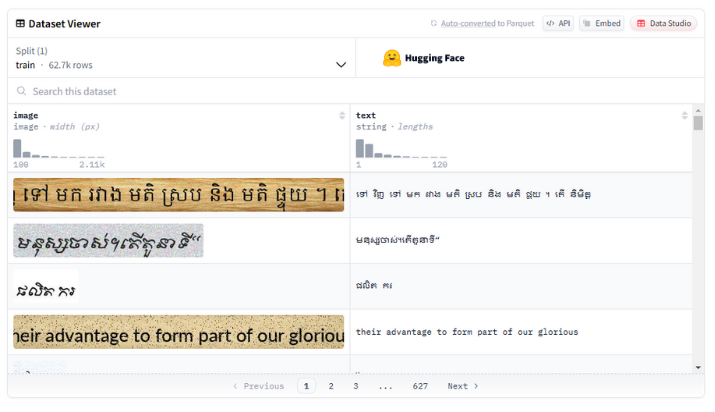
\includegraphics[width=1\textwidth]{figures/khmer_ocr_hugginface_dataset.png}
    \caption{The Khmer-Printed-Text-Dataset (62k images) used for model training and evaluation.}
    \label{fig:khmer_ocr_hugginface_dataset}
\end{figure}

\begin{figure}[H]
    \centering
    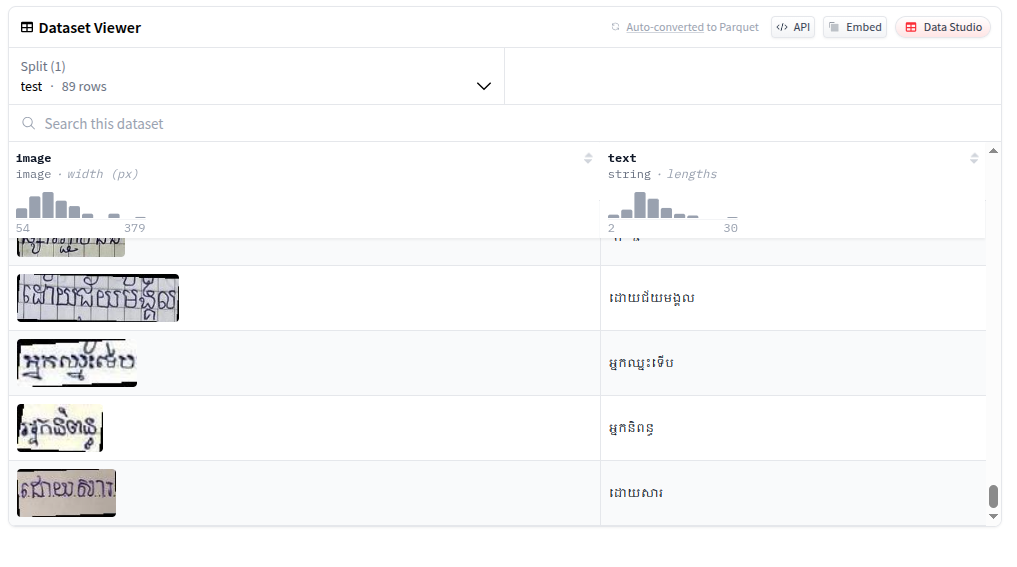
\includegraphics[width=1\textwidth]{figures/khmer_ocr_hugginface_dataset_2.png}
    \caption{The Datasets-KiteAether-up-khmer-gemma-ocr-Evalution-set used for evaluation on Khmer handwritten model, there are 89 images.}
    \label{fig:khmer_ocr_hugginface_dataset_2}
\end{figure}


These datasets enable a variety of OCR research and development tasks, including model training, validation, evaluation, and benchmarking. Researchers and developers can use them to train deep learning models for recognizing Khmer script, conduct font-style generalization studies, assess handwritten text recognition performance, and build production-grade Khmer OCR systems tailored to both digital and scanned documents.


\clearpage
\phantomsection
\label{appendix-b}
\section*{Appendix B: List of Fonts Used}

This appendix lists the Khmer and Latin fonts used during synthetic data generation and model evaluation. Font variability was critical for improving the model's ability to generalize across diverse document styles, layouts, and font renderings. Using a broad range of typefaces helps simulate real-world OCR scenarios, enhancing robustness and accuracy.

\begin{itemize}
    \item \textbf{Source 1 – Google Fonts (Khmer Collection)}  
    A wide variety of Khmer Unicode fonts were collected from Google Fonts.  
    \url{https://fonts.google.com/specimen/Khmer}

    \item \textbf{Source 2 – FontSC Cambodian Fonts Collection}  
    Additional Khmer and Cambodian-style fonts were gathered from this free font archive.  
    \url{https://www.fontsc.com/font/tag/cambodian}
\end{itemize}



\clearpage
\phantomsection
\label{appendix-d}
\section*{Appendix D: Previous Research Using TrOCR}

This appendix highlights prior research efforts related to Khmer handwriting recognition using the TrOCR architecture. The following study represents an important contribution to extending OCR capabilities beyond printed Khmer text.

\vspace{0.3cm}

\textbf{Title:} Khmer Handwritten OCR using Pretrained TrOCR Architecture  
\textbf{Authors:} Soy Vitou, Y Kimly, Lany Malis, Chean Botum  
\textbf{Advisor:} Kor Sokchea  
\textbf{Affiliation:} Department of Information Technology Engineering, Faculty of Engineering, Royal University of Phnom Penh  
\textbf{Project Year:} Year 3

\vspace{0.3cm}

\textbf{Abstract:}  
Most existing OCR models for the Khmer language focus solely on printed text, leaving handwritten text recognition largely unexplored. This limitation reduces OCR's usefulness in areas where handwritten forms are common, such as in schools, government offices, and traditional documents—resulting in inefficiencies due to manual data entry.

This research aimed to:
\begin{itemize}
    \item Develop an OCR model for Khmer handwritten text.
    \item Apply machine learning techniques to improve recognition accuracy.
    \item Bridge the gap between printed and handwritten Khmer OCR applications.
\end{itemize}

While OCR technology has seen significant progress for languages like English in both printed and handwritten forms, Khmer OCR remains underdeveloped, especially for handwriting. To address this, the study developed a Khmer handwritten OCR model using the pretrained TrOCR architecture.

A synthetic dataset of 50,000 printed Khmer text samples was generated using data augmentation techniques—such as noise addition, varied backgrounds, and font variations—for pretraining. A smaller, manually collected dataset of handwritten Khmer samples was then used for fine-tuning the model.

The resulting system demonstrated promising results, achieving a Character Error Rate (CER) of 0.17. Although the model showed an ability to recognize Khmer handwritten text, further improvement is possible through additional fine-tuning and expansion of the training data.

\vspace{0.3cm}

\textbf{Reference:}  
Khmer Handwritten OCR using Pretrained TrOCR Architecture.  
Available at: \url{https://www.researchgate.net/publication/385417010_Khmer_Handwritten_OCR_using_Pretrained_TrOCR_Architecture}  
[Accessed: June 19, 2025]

\end{document}
